\documentclass[lettersize,journal]{IEEEtran}
\usepackage{amsmath,amsfonts,amssymb}
\usepackage{algorithm}
\usepackage[noend]{algpseudocode}
\usepackage{array}
\usepackage[caption=false,font=normalsize,labelfont=sf,textfont=sf]{subfig}
\usepackage{textcomp}
\usepackage{stfloats}
\usepackage{url}
\usepackage{verbatim}
\usepackage{graphicx}
\usepackage{cite}
\usepackage{booktabs}
\usepackage{multirow}
\usepackage{xcolor}
\usepackage{tikz}
\usetikzlibrary{arrows.meta,positioning,fit,backgrounds,calc,shapes.geometric}
\usepackage{pgfplots}
\pgfplotsset{compat=1.18}
\hyphenation{op-tical net-works semi-conduc-tor IEEE-Xplore}
\algrenewcommand\algorithmicrequire{\textbf{Input:}}
\algrenewcommand\algorithmicensure{\textbf{Output:}}
\newcommand{\sys}{\textsc{Heartness}}
\newcommand{\src}{\mathit{src}}
\newcommand{\dep}{\mathit{dep}}
\newcommand{\expr}{\mathit{exp}}
\newcommand{\ctx}{\mathit{ctx}}
\newcommand{\run}{\mathit{run}}
\newcommand{\Cl}{\mathrm{Cl}}
\newcommand{\Act}{\mathit{Act}}
\newcommand{\Dpl}{\mathit{Dpl}}
\newcommand{\RQ}[1]{\textbf{RQ#1}}
\newtheorem{proposition}{Proposition}
\DeclareRobustCommand{\circled}[1]{\tikz[baseline=(c.base)]\node[circle,draw,inner sep=0.6pt,font=\scriptsize](c){#1};}

%% BEGIN GENERATED MACROS (scripts/paper_macros.py; do not edit by hand)
\newcommand{\LineCoverage}{98.4}
\newcommand{\BranchCoverage}{94.6}
\newcommand{\TestCount}{60}
\newcommand{\MutationKilled}{14}
\newcommand{\MutationTotal}{14}
\newcommand{\PublicRevisions}{12}
\newcommand{\PublicEvents}{36}
\newcommand{\LiveEvalTasks}{29}
\newcommand{\LiveEvolveTasks}{24}
\newcommand{\LiveSeeds}{5}
\newcommand{\LiveModels}{5}
\newcommand{\LivePolicies}{2}
\newcommand{\LiveTotalRuns}{200}
\newcommand{\LiveFaultyRuns}{150}
\newcommand{\LiveCleanRuns}{50}
\newcommand{\LiveLLMCalls}{42{,}811}
\newcommand{\LiveGPU}{H100 80GB HBM3}
\newcommand{\LiveConditions}{15}
\newcommand{\SrcLines}{1{,}209}
\newcommand{\LiveHarnessLines}{1{,}800}
\newcommand{\LiveEvalConditions}{11}
\newcommand{\LiveCOracleCells}{25}
\newcommand{\LiveCCPUCells}{2}
\newcommand{\TauTfidf}{0.05}
\newcommand{\TauEmbed}{0.55}
\newcommand{\TauTfidfDev}{0.575}
\newcommand{\TauEmbedDev}{0.625}
\newcommand{\PilotDevRuns}{6}
\newcommand{\RawRecords}{1{,}905}
\newcommand{\TraceCases}{810}
\newcommand{\SynHistoryImpact}{0.155}
\newcommand{\SynHistoryOrigins}{0.176}
\newcommand{\SynHistoryDescendants}{0.108}
\newcommand{\SynLexicalImpact}{0.699}
\newcommand{\SynLexicalOrigins}{0.374}
\newcommand{\SynLexicalDescendants}{0.607}
\newcommand{\SynCaptureOnlyImpact}{1.000}
\newcommand{\SynCaptureOnlyOrigins}{1.000}
\newcommand{\SynCaptureOnlyDescendants}{1.000}
\newcommand{\SynOursImpact}{1.000}
\newcommand{\SynOursOrigins}{1.000}
\newcommand{\SynOursDescendants}{1.000}
\newcommand{\CaptureOursZero}{0.103}
\newcommand{\CaptureLexicalZero}{0.687}
\newcommand{\CaptureHistoryZero}{0.035}
\newcommand{\CaptureOursQuarter}{0.289}
\newcommand{\CaptureLexicalQuarter}{0.687}
\newcommand{\CaptureHistoryQuarter}{0.035}
\newcommand{\CaptureOursHalf}{0.572}
\newcommand{\CaptureLexicalHalf}{0.687}
\newcommand{\CaptureHistoryHalf}{0.035}
\newcommand{\CaptureOursThreeQuarters}{0.833}
\newcommand{\CaptureLexicalThreeQuarters}{0.687}
\newcommand{\CaptureHistoryThreeQuarters}{0.035}
\newcommand{\CaptureOursFull}{1.000}
\newcommand{\CaptureLexicalFull}{0.687}
\newcommand{\CaptureHistoryFull}{0.035}
\newcommand{\ParaOursZero}{1.000}
\newcommand{\ParaLexicalZero}{0.755}
\newcommand{\ParaOursHalf}{1.000}
\newcommand{\ParaLexicalHalf}{0.687}
\newcommand{\ParaOursFull}{1.000}
\newcommand{\ParaLexicalFull}{0.689}
\newcommand{\CheckerComparisons}{18}
\newcommand{\CheckerAgreements}{18}
\newcommand{\CheckerViolating}{13}
\newcommand{\CheckerSafeMutants}{2}
\newcommand{\Counterexamples}{13}
\newcommand{\ReplaySuccesses}{13}
\newcommand{\MinimalWitnesses}{13}
\newcommand{\WitnessMin}{2}
\newcommand{\WitnessMax}{7}
\newcommand{\MaxReferenceStates}{93{,}266}
\newcommand{\MappedTransitions}{3{,}000}
\newcommand{\MappedEnabled}{992}
\newcommand{\MappedMismatches}{0}
\newcommand{\LinterFOne}{0.229}
\newcommand{\LinterCases}{90}
\newcommand{\LinterBenign}{0}
\newcommand{\MonDrift}{30}
\newcommand{\MonInvalid}{30}
\newcommand{\MonOmitted}{29}
\newcommand{\MonHidden}{0}
\newcommand{\MonBenign}{0}
\newcommand{\MonN}{30}
\newcommand{\RemediationRuns}{30}
\newcommand{\UnsafeRollbackRejected}{30}
\newcommand{\EffectsRetained}{30}
\newcommand{\GraphMilliseconds}{28.14}
\newcommand{\GraphKilobytes}{1055}
\newcommand{\AdmissionMsThirtyTwo}{1134.8}
\newcommand{\AdmissionMsFour}{28.0}
\newcommand{\WithdrawalMsThirtyTwo}{22.7}
\newcommand{\WithdrawalMsFour}{2.7}
\newcommand{\MonitorMsThirtyTwo}{2967.7}
\newcommand{\MonitorMsFour}{48.1}
\newcommand{\CaptureMsThirtyTwo}{1.7}
\newcommand{\CaptureMsFour}{0.2}
\newcommand{\HistoryEventsThirtyTwo}{105}
\newcommand{\GuardChallenges}{10}
\newcommand{\GuardRemovedAlarms}{10}
\newcommand{\LiveERuns}{75}
\newcommand{\LiveEPropagated}{10}
\newcommand{\LiveERootAdopted}{21}
\newcommand{\LiveEContaminated}{16}
\newcommand{\LiveEAmbiguous}{0}
\newcommand{\LiveEMeanArtifacts}{8.0}
\newcommand{\LiveEKappa}{0.99}
\newcommand{\LiveEJudgeItems}{1384}
\newcommand{\LiveEJudgeRaw}{99.9}
\newcommand{\LiveEJudgePositive}{0.99}
\newcommand{\LiveEHSjudgeDiffersRfour}{2}
\newcommand{\LiveEPassClean}{0.61}
\newcommand{\LiveEPassSeed}{0.63}
\newcommand{\LiveECleanFalseLabels}{0}
\newcommand{\LiveECleanLabelItems}{630}
\newcommand{\LiveECleanAmbLabels}{0}
\newcommand{\LiveEBoundTfidfRec}{1.00}
\newcommand{\LiveEBoundEmbedRec}{1.00}
\newcommand{\LiveENoneRec}{0.00}
\newcommand{\LiveENoneFone}{0.00}
\newcommand{\LiveENoneResid}{0.21}
\newcommand{\LiveENoneColl}{0.00}
\newcommand{\LiveENonePass}{0.59}
\newcommand{\LiveENoneSig}{0.03}
\newcommand{\LiveENoneSusp}{0.00}
\newcommand{\LiveENoneSuspProp}{0.00}
\newcommand{\LiveENoneCollProp}{0.00}
\newcommand{\LiveENonePassProp}{0.60}
\newcommand{\LiveENoneSigProp}{0.09}
\newcommand{\LiveENoneRecAmb}{0.00}
\newcommand{\LiveERoneRec}{0.00}
\newcommand{\LiveERoneFone}{0.00}
\newcommand{\LiveERoneResid}{0.21}
\newcommand{\LiveERoneColl}{0.00}
\newcommand{\LiveERonePass}{0.59}
\newcommand{\LiveERoneSig}{0.03}
\newcommand{\LiveERoneSusp}{0.00}
\newcommand{\LiveERoneSuspProp}{0.00}
\newcommand{\LiveERoneCollProp}{0.00}
\newcommand{\LiveERonePassProp}{0.60}
\newcommand{\LiveERoneSigProp}{0.09}
\newcommand{\LiveERoneRecAmb}{0.00}
\newcommand{\LiveERtwoPrec}{0.07}
\newcommand{\LiveERtwoRec}{1.00}
\newcommand{\LiveERtwoFone}{0.60}
\newcommand{\LiveERtwoResid}{0.00}
\newcommand{\LiveERtwoColl}{4.76}
\newcommand{\LiveERtwoPass}{0.60}
\newcommand{\LiveERtwoSig}{0.02}
\newcommand{\LiveERtwoSusp}{4.97}
\newcommand{\LiveERtwoPrecProp}{0.50}
\newcommand{\LiveERtwoSuspProp}{4.20}
\newcommand{\LiveERtwoCollProp}{2.60}
\newcommand{\LiveERtwoPassProp}{0.67}
\newcommand{\LiveERtwoSigProp}{0.02}
\newcommand{\LiveERtwoRecAmb}{1.00}
\newcommand{\LiveERthreePrec}{0.05}
\newcommand{\LiveERthreeRec}{1.00}
\newcommand{\LiveERthreeFone}{0.50}
\newcommand{\LiveERthreeResid}{0.00}
\newcommand{\LiveERthreeColl}{5.93}
\newcommand{\LiveERthreePass}{0.61}
\newcommand{\LiveERthreeSig}{0.02}
\newcommand{\LiveERthreeSusp}{6.15}
\newcommand{\LiveERthreePrecProp}{0.39}
\newcommand{\LiveERthreeSuspProp}{5.30}
\newcommand{\LiveERthreeCollProp}{3.70}
\newcommand{\LiveERthreePassProp}{0.69}
\newcommand{\LiveERthreeSigProp}{0.02}
\newcommand{\LiveERthreeRecAmb}{1.00}
\newcommand{\LiveERfourPrec}{0.10}
\newcommand{\LiveERfourRec}{0.90}
\newcommand{\LiveERfourFone}{0.65}
\newcommand{\LiveERfourResid}{0.01}
\newcommand{\LiveERfourColl}{2.39}
\newcommand{\LiveERfourPass}{0.60}
\newcommand{\LiveERfourSig}{0.02}
\newcommand{\LiveERfourSusp}{2.59}
\newcommand{\LiveERfourPrecProp}{0.55}
\newcommand{\LiveERfourSuspProp}{3.70}
\newcommand{\LiveERfourCollProp}{2.20}
\newcommand{\LiveERfourPassProp}{0.68}
\newcommand{\LiveERfourSigProp}{0.02}
\newcommand{\LiveERfourRecAmb}{0.90}
\newcommand{\LiveEHPrec}{0.04}
\newcommand{\LiveEHRec}{1.00}
\newcommand{\LiveEHFone}{0.48}
\newcommand{\LiveEHResid}{0.00}
\newcommand{\LiveEHColl}{5.73}
\newcommand{\LiveEHPass}{0.62}
\newcommand{\LiveEHSig}{0.02}
\newcommand{\LiveEHSusp}{5.95}
\newcommand{\LiveEHPrecProp}{0.33}
\newcommand{\LiveEHSuspProp}{4.90}
\newcommand{\LiveEHCollProp}{3.30}
\newcommand{\LiveEHPassProp}{0.68}
\newcommand{\LiveEHSigProp}{0.02}
\newcommand{\LiveEHRecAmb}{1.00}
\newcommand{\LiveEHnoEMEPrec}{0.04}
\newcommand{\LiveEHnoEMERec}{1.00}
\newcommand{\LiveEHnoEMEFone}{0.48}
\newcommand{\LiveEHnoEMEResid}{0.00}
\newcommand{\LiveEHnoEMEColl}{5.73}
\newcommand{\LiveEHnoEMEPass}{0.62}
\newcommand{\LiveEHnoEMESig}{0.02}
\newcommand{\LiveEHnoEMESusp}{5.95}
\newcommand{\LiveEHnoEMEPrecProp}{0.33}
\newcommand{\LiveEHnoEMESuspProp}{4.90}
\newcommand{\LiveEHnoEMECollProp}{3.30}
\newcommand{\LiveEHnoEMEPassProp}{0.68}
\newcommand{\LiveEHnoEMESigProp}{0.02}
\newcommand{\LiveEHnoEMERecAmb}{1.00}
\newcommand{\LiveEHnoDepsPrec}{0.04}
\newcommand{\LiveEHnoDepsRec}{1.00}
\newcommand{\LiveEHnoDepsFone}{0.48}
\newcommand{\LiveEHnoDepsResid}{0.00}
\newcommand{\LiveEHnoDepsColl}{5.73}
\newcommand{\LiveEHnoDepsPass}{0.62}
\newcommand{\LiveEHnoDepsSig}{0.02}
\newcommand{\LiveEHnoDepsSusp}{5.95}
\newcommand{\LiveEHnoDepsPrecProp}{0.33}
\newcommand{\LiveEHnoDepsSuspProp}{4.90}
\newcommand{\LiveEHnoDepsCollProp}{3.30}
\newcommand{\LiveEHnoDepsPassProp}{0.68}
\newcommand{\LiveEHnoDepsSigProp}{0.02}
\newcommand{\LiveEHnoDepsRecAmb}{1.00}
\newcommand{\LiveEHlocalRec}{0.00}
\newcommand{\LiveEHlocalFone}{0.00}
\newcommand{\LiveEHlocalResid}{0.21}
\newcommand{\LiveEHlocalColl}{0.00}
\newcommand{\LiveEHlocalPass}{0.59}
\newcommand{\LiveEHlocalSig}{0.03}
\newcommand{\LiveEHlocalSusp}{0.00}
\newcommand{\LiveEHlocalSuspProp}{0.00}
\newcommand{\LiveEHlocalCollProp}{0.00}
\newcommand{\LiveEHlocalPassProp}{0.60}
\newcommand{\LiveEHlocalSigProp}{0.09}
\newcommand{\LiveEHlocalRecAmb}{0.00}
\newcommand{\LiveEHSjudgePrec}{0.11}
\newcommand{\LiveEHSjudgeRec}{0.90}
\newcommand{\LiveEHSjudgeFone}{0.67}
\newcommand{\LiveEHSjudgeResid}{0.01}
\newcommand{\LiveEHSjudgeColl}{2.16}
\newcommand{\LiveEHSjudgePass}{0.60}
\newcommand{\LiveEHSjudgeSig}{0.02}
\newcommand{\LiveEHSjudgeSusp}{2.36}
\newcommand{\LiveEHSjudgePrecProp}{0.59}
\newcommand{\LiveEHSjudgeSuspProp}{3.50}
\newcommand{\LiveEHSjudgeCollProp}{2.00}
\newcommand{\LiveEHSjudgePassProp}{0.68}
\newcommand{\LiveEHSjudgeSigProp}{0.02}
\newcommand{\LiveEHSjudgeRecAmb}{0.90}
\newcommand{\LiveEHSembedPrec}{0.07}
\newcommand{\LiveEHSembedRec}{1.00}
\newcommand{\LiveEHSembedFone}{0.62}
\newcommand{\LiveEHSembedResid}{0.00}
\newcommand{\LiveEHSembedColl}{4.59}
\newcommand{\LiveEHSembedPass}{0.61}
\newcommand{\LiveEHSembedSig}{0.02}
\newcommand{\LiveEHSembedSusp}{4.80}
\newcommand{\LiveEHSembedPrecProp}{0.51}
\newcommand{\LiveEHSembedSuspProp}{4.10}
\newcommand{\LiveEHSembedCollProp}{2.50}
\newcommand{\LiveEHSembedPassProp}{0.70}
\newcommand{\LiveEHSembedSigProp}{0.02}
\newcommand{\LiveEHSembedRecAmb}{1.00}
\newcommand{\LiveETcutPrec}{0.04}
\newcommand{\LiveETcutRec}{1.00}
\newcommand{\LiveETcutFone}{0.48}
\newcommand{\LiveETcutResid}{0.00}
\newcommand{\LiveETcutColl}{5.73}
\newcommand{\LiveETcutSusp}{5.95}
\newcommand{\LiveETcutPrecProp}{0.33}
\newcommand{\LiveETcutSuspProp}{4.90}
\newcommand{\LiveETcutCollProp}{3.30}
\newcommand{\LiveETcutRecAmb}{1.00}
\newcommand{\LiveEAresetPrec}{0.04}
\newcommand{\LiveEAresetRec}{1.00}
\newcommand{\LiveEAresetFone}{0.47}
\newcommand{\LiveEAresetResid}{0.00}
\newcommand{\LiveEAresetColl}{5.79}
\newcommand{\LiveEAresetSusp}{6.00}
\newcommand{\LiveEAresetPrecProp}{0.33}
\newcommand{\LiveEAresetSuspProp}{5.00}
\newcommand{\LiveEAresetCollProp}{3.40}
\newcommand{\LiveEAresetRecAmb}{1.00}
\newcommand{\LiveEHfaultyPrec}{0.16}
\newcommand{\LiveEHfaultyRec}{1.00}
\newcommand{\LiveEHfaultyFone}{0.48}
\newcommand{\LiveEHfaultyResid}{0.00}
\newcommand{\LiveEHfaultyColl}{1.17}
\newcommand{\LiveEHfaultySusp}{1.39}
\newcommand{\LiveEHfaultyPrecProp}{0.33}
\newcommand{\LiveEHfaultySuspProp}{4.90}
\newcommand{\LiveEHfaultyCollProp}{3.30}
\newcommand{\LiveEHfaultyRecAmb}{1.00}
\newcommand{\LiveEHEMEfailPrec}{0.04}
\newcommand{\LiveEHEMEfailRec}{1.00}
\newcommand{\LiveEHEMEfailFone}{0.48}
\newcommand{\LiveEHEMEfailResid}{0.00}
\newcommand{\LiveEHEMEfailColl}{5.73}
\newcommand{\LiveEHEMEfailSusp}{5.95}
\newcommand{\LiveEHEMEfailPrecProp}{0.33}
\newcommand{\LiveEHEMEfailSuspProp}{4.90}
\newcommand{\LiveEHEMEfailCollProp}{3.30}
\newcommand{\LiveEHEMEfailRecAmb}{1.00}
\newcommand{\LiveENoneMs}{0.0}
\newcommand{\LiveERoneMs}{0.0}
\newcommand{\LiveERtwoMs}{1.1}
\newcommand{\LiveERthreeMs}{3014.3}
\newcommand{\LiveERfourMs}{20614.6}
\newcommand{\LiveEHMs}{20.3}
\newcommand{\LiveEHnoEMEMs}{33.1}
\newcommand{\LiveEHnoDepsMs}{0.4}
\newcommand{\LiveEHlocalMs}{29.7}
\newcommand{\LiveEHSjudgeMs}{0.0}
\newcommand{\LiveEHSembedMs}{0.0}
\newcommand{\LiveETcutMs}{0.0}
\newcommand{\LiveEAresetMs}{0.0}
\newcommand{\LiveEHfaultyMs}{0.0}
\newcommand{\LiveEHEMEfailMs}{0.0}
\newcommand{\LiveETestResidNoneP}{=0.025}
\newcommand{\LiveETestResidNoneHi}{0}
\newcommand{\LiveETestResidNoneLo}{10}
\newcommand{\LiveETestResidNoneA}{0.43}
\newcommand{\LiveETestResidRoneP}{=0.025}
\newcommand{\LiveETestResidRoneHi}{0}
\newcommand{\LiveETestResidRoneLo}{10}
\newcommand{\LiveETestResidRoneA}{0.43}
\newcommand{\LiveETestResidRtwoP}{=1.000}
\newcommand{\LiveETestResidRtwoHi}{0}
\newcommand{\LiveETestResidRtwoLo}{0}
\newcommand{\LiveETestResidRtwoA}{0.50}
\newcommand{\LiveETestResidRthreeP}{=1.000}
\newcommand{\LiveETestResidRthreeHi}{0}
\newcommand{\LiveETestResidRthreeLo}{0}
\newcommand{\LiveETestResidRthreeA}{0.50}
\newcommand{\LiveETestResidRfourP}{=1.000}
\newcommand{\LiveETestResidRfourHi}{0}
\newcommand{\LiveETestResidRfourLo}{1}
\newcommand{\LiveETestResidRfourA}{0.49}
\newcommand{\LiveETestResidHnoEMEP}{--}
\newcommand{\LiveETestResidHnoEMEHi}{0}
\newcommand{\LiveETestResidHnoEMELo}{0}
\newcommand{\LiveETestResidHnoEMEA}{0.50}
\newcommand{\LiveETestResidHnoDepsP}{--}
\newcommand{\LiveETestResidHnoDepsHi}{0}
\newcommand{\LiveETestResidHnoDepsLo}{0}
\newcommand{\LiveETestResidHnoDepsA}{0.50}
\newcommand{\LiveETestResidHlocalP}{--}
\newcommand{\LiveETestResidHlocalHi}{0}
\newcommand{\LiveETestResidHlocalLo}{10}
\newcommand{\LiveETestResidHlocalA}{0.43}
\newcommand{\LiveETestResidHSjudgeP}{=1.000}
\newcommand{\LiveETestResidHSjudgeHi}{0}
\newcommand{\LiveETestResidHSjudgeLo}{1}
\newcommand{\LiveETestResidHSjudgeA}{0.49}
\newcommand{\LiveETestResidHSembedP}{=1.000}
\newcommand{\LiveETestResidHSembedHi}{0}
\newcommand{\LiveETestResidHSembedLo}{0}
\newcommand{\LiveETestResidHSembedA}{0.50}
\newcommand{\LiveETestResidTcutP}{--}
\newcommand{\LiveETestResidTcutHi}{0}
\newcommand{\LiveETestResidTcutLo}{0}
\newcommand{\LiveETestResidTcutA}{0.50}
\newcommand{\LiveETestResidAresetP}{--}
\newcommand{\LiveETestResidAresetHi}{0}
\newcommand{\LiveETestResidAresetLo}{0}
\newcommand{\LiveETestResidAresetA}{0.50}
\newcommand{\LiveETestResidHfaultyP}{--}
\newcommand{\LiveETestResidHfaultyHi}{0}
\newcommand{\LiveETestResidHfaultyLo}{0}
\newcommand{\LiveETestResidHfaultyA}{0.50}
\newcommand{\LiveETestResidHEMEfailP}{--}
\newcommand{\LiveETestResidHEMEfailHi}{0}
\newcommand{\LiveETestResidHEMEfailLo}{0}
\newcommand{\LiveETestResidHEMEfailA}{0.50}
\newcommand{\LiveETestRecNoneP}{=0.014}
\newcommand{\LiveETestRecNoneHi}{10}
\newcommand{\LiveETestRecNoneLo}{0}
\newcommand{\LiveETestRecNoneA}{1.00}
\newcommand{\LiveETestRecRoneP}{=0.014}
\newcommand{\LiveETestRecRoneHi}{10}
\newcommand{\LiveETestRecRoneLo}{0}
\newcommand{\LiveETestRecRoneA}{1.00}
\newcommand{\LiveETestRecRtwoP}{=1.000}
\newcommand{\LiveETestRecRtwoHi}{0}
\newcommand{\LiveETestRecRtwoLo}{0}
\newcommand{\LiveETestRecRtwoA}{0.50}
\newcommand{\LiveETestRecRthreeP}{=1.000}
\newcommand{\LiveETestRecRthreeHi}{0}
\newcommand{\LiveETestRecRthreeLo}{0}
\newcommand{\LiveETestRecRthreeA}{0.50}
\newcommand{\LiveETestRecRfourP}{=1.000}
\newcommand{\LiveETestRecRfourHi}{1}
\newcommand{\LiveETestRecRfourLo}{0}
\newcommand{\LiveETestRecRfourA}{0.55}
\newcommand{\LiveETestRecHnoEMEP}{--}
\newcommand{\LiveETestRecHnoEMEHi}{0}
\newcommand{\LiveETestRecHnoEMELo}{0}
\newcommand{\LiveETestRecHnoEMEA}{0.50}
\newcommand{\LiveETestRecHnoDepsP}{--}
\newcommand{\LiveETestRecHnoDepsHi}{0}
\newcommand{\LiveETestRecHnoDepsLo}{0}
\newcommand{\LiveETestRecHnoDepsA}{0.50}
\newcommand{\LiveETestRecHlocalP}{--}
\newcommand{\LiveETestRecHlocalHi}{10}
\newcommand{\LiveETestRecHlocalLo}{0}
\newcommand{\LiveETestRecHlocalA}{1.00}
\newcommand{\LiveETestRecHSjudgeP}{=1.000}
\newcommand{\LiveETestRecHSjudgeHi}{1}
\newcommand{\LiveETestRecHSjudgeLo}{0}
\newcommand{\LiveETestRecHSjudgeA}{0.55}
\newcommand{\LiveETestRecHSembedP}{=1.000}
\newcommand{\LiveETestRecHSembedHi}{0}
\newcommand{\LiveETestRecHSembedLo}{0}
\newcommand{\LiveETestRecHSembedA}{0.50}
\newcommand{\LiveETestRecTcutP}{--}
\newcommand{\LiveETestRecTcutHi}{0}
\newcommand{\LiveETestRecTcutLo}{0}
\newcommand{\LiveETestRecTcutA}{0.50}
\newcommand{\LiveETestRecAresetP}{--}
\newcommand{\LiveETestRecAresetHi}{0}
\newcommand{\LiveETestRecAresetLo}{0}
\newcommand{\LiveETestRecAresetA}{0.50}
\newcommand{\LiveETestRecHfaultyP}{--}
\newcommand{\LiveETestRecHfaultyHi}{0}
\newcommand{\LiveETestRecHfaultyLo}{0}
\newcommand{\LiveETestRecHfaultyA}{0.50}
\newcommand{\LiveETestRecHEMEfailP}{--}
\newcommand{\LiveETestRecHEMEfailHi}{0}
\newcommand{\LiveETestRecHEMEfailLo}{0}
\newcommand{\LiveETestRecHEMEfailA}{0.50}
\newcommand{\LiveETestPassNoneP}{=0.056}
\newcommand{\LiveETestPassNoneHi}{37}
\newcommand{\LiveETestPassNoneLo}{22}
\newcommand{\LiveETestPassNoneA}{0.56}
\newcommand{\LiveETestPassRoneP}{=0.078}
\newcommand{\LiveETestPassRoneHi}{35}
\newcommand{\LiveETestPassRoneLo}{23}
\newcommand{\LiveETestPassRoneA}{0.56}
\newcommand{\LiveETestPassRtwoP}{=0.148}
\newcommand{\LiveETestPassRtwoHi}{26}
\newcommand{\LiveETestPassRtwoLo}{16}
\newcommand{\LiveETestPassRtwoA}{0.53}
\newcommand{\LiveETestPassRthreeP}{=0.506}
\newcommand{\LiveETestPassRthreeHi}{17}
\newcommand{\LiveETestPassRthreeLo}{15}
\newcommand{\LiveETestPassRthreeA}{0.52}
\newcommand{\LiveETestPassRfourP}{=0.153}
\newcommand{\LiveETestPassRfourHi}{34}
\newcommand{\LiveETestPassRfourLo}{20}
\newcommand{\LiveETestPassRfourA}{0.54}
\newcommand{\LiveETestPassHnoEMEP}{--}
\newcommand{\LiveETestPassHnoEMEHi}{0}
\newcommand{\LiveETestPassHnoEMELo}{0}
\newcommand{\LiveETestPassHnoEMEA}{0.50}
\newcommand{\LiveETestPassHnoDepsP}{--}
\newcommand{\LiveETestPassHnoDepsHi}{0}
\newcommand{\LiveETestPassHnoDepsLo}{0}
\newcommand{\LiveETestPassHnoDepsA}{0.50}
\newcommand{\LiveETestPassHlocalP}{--}
\newcommand{\LiveETestPassHlocalHi}{37}
\newcommand{\LiveETestPassHlocalLo}{22}
\newcommand{\LiveETestPassHlocalA}{0.56}
\newcommand{\LiveETestPassHSjudgeP}{=0.153}
\newcommand{\LiveETestPassHSjudgeHi}{34}
\newcommand{\LiveETestPassHSjudgeLo}{22}
\newcommand{\LiveETestPassHSjudgeA}{0.54}
\newcommand{\LiveETestPassHSembedP}{=0.848}
\newcommand{\LiveETestPassHSembedHi}{20}
\newcommand{\LiveETestPassHSembedLo}{26}
\newcommand{\LiveETestPassHSembedA}{0.50}
\newcommand{\LiveETestCollNoneP}{<0.001}
\newcommand{\LiveETestCollNoneHi}{75}
\newcommand{\LiveETestCollNoneLo}{0}
\newcommand{\LiveETestCollNoneA}{1.00}
\newcommand{\LiveETestCollRoneP}{<0.001}
\newcommand{\LiveETestCollRoneHi}{75}
\newcommand{\LiveETestCollRoneLo}{0}
\newcommand{\LiveETestCollRoneA}{1.00}
\newcommand{\LiveETestCollRtwoP}{<0.001}
\newcommand{\LiveETestCollRtwoHi}{46}
\newcommand{\LiveETestCollRtwoLo}{16}
\newcommand{\LiveETestCollRtwoA}{0.64}
\newcommand{\LiveETestCollRthreeP}{=0.207}
\newcommand{\LiveETestCollRthreeHi}{23}
\newcommand{\LiveETestCollRthreeLo}{40}
\newcommand{\LiveETestCollRthreeA}{0.45}
\newcommand{\LiveETestCollRfourP}{<0.001}
\newcommand{\LiveETestCollRfourHi}{63}
\newcommand{\LiveETestCollRfourLo}{4}
\newcommand{\LiveETestCollRfourA}{0.83}
\newcommand{\LiveETestCollHnoEMEP}{--}
\newcommand{\LiveETestCollHnoEMEHi}{0}
\newcommand{\LiveETestCollHnoEMELo}{0}
\newcommand{\LiveETestCollHnoEMEA}{0.50}
\newcommand{\LiveETestCollHnoDepsP}{--}
\newcommand{\LiveETestCollHnoDepsHi}{0}
\newcommand{\LiveETestCollHnoDepsLo}{0}
\newcommand{\LiveETestCollHnoDepsA}{0.50}
\newcommand{\LiveETestCollHlocalP}{--}
\newcommand{\LiveETestCollHlocalHi}{75}
\newcommand{\LiveETestCollHlocalLo}{0}
\newcommand{\LiveETestCollHlocalA}{1.00}
\newcommand{\LiveETestCollHSjudgeP}{<0.001}
\newcommand{\LiveETestCollHSjudgeHi}{64}
\newcommand{\LiveETestCollHSjudgeLo}{0}
\newcommand{\LiveETestCollHSjudgeA}{0.85}
\newcommand{\LiveETestCollHSembedP}{<0.001}
\newcommand{\LiveETestCollHSembedHi}{41}
\newcommand{\LiveETestCollHSembedLo}{0}
\newcommand{\LiveETestCollHSembedA}{0.65}
\newcommand{\LiveETestCollTcutP}{--}
\newcommand{\LiveETestCollTcutHi}{0}
\newcommand{\LiveETestCollTcutLo}{0}
\newcommand{\LiveETestCollTcutA}{0.50}
\newcommand{\LiveETestCollAresetP}{--}
\newcommand{\LiveETestCollAresetHi}{0}
\newcommand{\LiveETestCollAresetLo}{4}
\newcommand{\LiveETestCollAresetA}{0.49}
\newcommand{\LiveETestCollHfaultyP}{--}
\newcommand{\LiveETestCollHfaultyHi}{54}
\newcommand{\LiveETestCollHfaultyLo}{0}
\newcommand{\LiveETestCollHfaultyA}{0.91}
\newcommand{\LiveETestCollHEMEfailP}{--}
\newcommand{\LiveETestCollHEMEfailHi}{0}
\newcommand{\LiveETestCollHEMEfailLo}{0}
\newcommand{\LiveETestCollHEMEfailA}{0.50}
\newcommand{\LiveETestFoneNoneP}{=0.014}
\newcommand{\LiveETestFoneNoneHi}{10}
\newcommand{\LiveETestFoneNoneLo}{0}
\newcommand{\LiveETestFoneNoneA}{1.00}
\newcommand{\LiveETestFoneRoneP}{=0.014}
\newcommand{\LiveETestFoneRoneHi}{10}
\newcommand{\LiveETestFoneRoneLo}{0}
\newcommand{\LiveETestFoneRoneA}{1.00}
\newcommand{\LiveETestFoneRtwoP}{=0.352}
\newcommand{\LiveETestFoneRtwoHi}{2}
\newcommand{\LiveETestFoneRtwoLo}{6}
\newcommand{\LiveETestFoneRtwoA}{0.41}
\newcommand{\LiveETestFoneRthreeP}{=0.945}
\newcommand{\LiveETestFoneRthreeHi}{5}
\newcommand{\LiveETestFoneRthreeLo}{3}
\newcommand{\LiveETestFoneRthreeA}{0.56}
\newcommand{\LiveETestFoneRfourP}{=0.273}
\newcommand{\LiveETestFoneRfourHi}{2}
\newcommand{\LiveETestFoneRfourLo}{7}
\newcommand{\LiveETestFoneRfourA}{0.29}
\newcommand{\LiveETestFoneHnoEMEP}{--}
\newcommand{\LiveETestFoneHnoEMEHi}{0}
\newcommand{\LiveETestFoneHnoEMELo}{0}
\newcommand{\LiveETestFoneHnoEMEA}{0.50}
\newcommand{\LiveETestFoneHnoDepsP}{--}
\newcommand{\LiveETestFoneHnoDepsHi}{0}
\newcommand{\LiveETestFoneHnoDepsLo}{0}
\newcommand{\LiveETestFoneHnoDepsA}{0.50}
\newcommand{\LiveETestFoneHlocalP}{--}
\newcommand{\LiveETestFoneHlocalHi}{10}
\newcommand{\LiveETestFoneHlocalLo}{0}
\newcommand{\LiveETestFoneHlocalA}{1.00}
\newcommand{\LiveETestFoneHSjudgeP}{=0.273}
\newcommand{\LiveETestFoneHSjudgeHi}{1}
\newcommand{\LiveETestFoneHSjudgeLo}{7}
\newcommand{\LiveETestFoneHSjudgeA}{0.28}
\newcommand{\LiveETestFoneHSembedP}{=0.352}
\newcommand{\LiveETestFoneHSembedHi}{0}
\newcommand{\LiveETestFoneHSembedLo}{4}
\newcommand{\LiveETestFoneHSembedA}{0.37}
\newcommand{\LiveETestFoneTcutP}{--}
\newcommand{\LiveETestFoneTcutHi}{0}
\newcommand{\LiveETestFoneTcutLo}{0}
\newcommand{\LiveETestFoneTcutA}{0.50}
\newcommand{\LiveETestFoneAresetP}{--}
\newcommand{\LiveETestFoneAresetHi}{1}
\newcommand{\LiveETestFoneAresetLo}{0}
\newcommand{\LiveETestFoneAresetA}{0.53}
\newcommand{\LiveETestFoneHfaultyP}{--}
\newcommand{\LiveETestFoneHfaultyHi}{0}
\newcommand{\LiveETestFoneHfaultyLo}{0}
\newcommand{\LiveETestFoneHfaultyA}{0.50}
\newcommand{\LiveETestFoneHEMEfailP}{--}
\newcommand{\LiveETestFoneHEMEfailHi}{0}
\newcommand{\LiveETestFoneHEMEfailLo}{0}
\newcommand{\LiveETestFoneHEMEfailA}{0.50}
\newcommand{\LiveETestSigNoneP}{=0.952}
\newcommand{\LiveETestSigNoneHi}{6}
\newcommand{\LiveETestSigNoneLo}{6}
\newcommand{\LiveETestSigNoneA}{0.50}
\newcommand{\LiveETestSigRoneP}{=0.952}
\newcommand{\LiveETestSigRoneHi}{7}
\newcommand{\LiveETestSigRoneLo}{6}
\newcommand{\LiveETestSigRoneA}{0.50}
\newcommand{\LiveETestSigRtwoP}{=0.952}
\newcommand{\LiveETestSigRtwoHi}{5}
\newcommand{\LiveETestSigRtwoLo}{1}
\newcommand{\LiveETestSigRtwoA}{0.52}
\newcommand{\LiveETestSigRthreeP}{=0.416}
\newcommand{\LiveETestSigRthreeHi}{3}
\newcommand{\LiveETestSigRthreeLo}{0}
\newcommand{\LiveETestSigRthreeA}{0.52}
\newcommand{\LiveETestSigRfourP}{=0.209}
\newcommand{\LiveETestSigRfourHi}{9}
\newcommand{\LiveETestSigRfourLo}{2}
\newcommand{\LiveETestSigRfourA}{0.54}
\newcommand{\LiveETestSigHnoEMEP}{--}
\newcommand{\LiveETestSigHnoEMEHi}{0}
\newcommand{\LiveETestSigHnoEMELo}{0}
\newcommand{\LiveETestSigHnoEMEA}{0.50}
\newcommand{\LiveETestSigHnoDepsP}{--}
\newcommand{\LiveETestSigHnoDepsHi}{0}
\newcommand{\LiveETestSigHnoDepsLo}{0}
\newcommand{\LiveETestSigHnoDepsA}{0.50}
\newcommand{\LiveETestSigHlocalP}{--}
\newcommand{\LiveETestSigHlocalHi}{6}
\newcommand{\LiveETestSigHlocalLo}{6}
\newcommand{\LiveETestSigHlocalA}{0.50}
\newcommand{\LiveETestSigHSjudgeP}{=0.137}
\newcommand{\LiveETestSigHSjudgeHi}{8}
\newcommand{\LiveETestSigHSjudgeLo}{1}
\newcommand{\LiveETestSigHSjudgeA}{0.54}
\newcommand{\LiveETestSigHSembedP}{=0.719}
\newcommand{\LiveETestSigHSembedHi}{4}
\newcommand{\LiveETestSigHSembedLo}{1}
\newcommand{\LiveETestSigHSembedA}{0.51}
\newcommand{\LiveETestPassPropNoneP}{=1.000}
\newcommand{\LiveETestPassPropNoneHi}{5}
\newcommand{\LiveETestPassPropNoneLo}{5}
\newcommand{\LiveETestPassPropNoneA}{0.70}
\newcommand{\LiveETestPassPropRoneP}{=1.000}
\newcommand{\LiveETestPassPropRoneHi}{5}
\newcommand{\LiveETestPassPropRoneLo}{5}
\newcommand{\LiveETestPassPropRoneA}{0.70}
\newcommand{\LiveETestPassPropRtwoP}{=1.000}
\newcommand{\LiveETestPassPropRtwoHi}{4}
\newcommand{\LiveETestPassPropRtwoLo}{3}
\newcommand{\LiveETestPassPropRtwoA}{0.53}
\newcommand{\LiveETestPassPropRthreeP}{=1.000}
\newcommand{\LiveETestPassPropRthreeHi}{1}
\newcommand{\LiveETestPassPropRthreeLo}{3}
\newcommand{\LiveETestPassPropRthreeA}{0.47}
\newcommand{\LiveETestPassPropRfourP}{=1.000}
\newcommand{\LiveETestPassPropRfourHi}{4}
\newcommand{\LiveETestPassPropRfourLo}{4}
\newcommand{\LiveETestPassPropRfourA}{0.54}
\newcommand{\LiveETestPassPropHnoEMEP}{--}
\newcommand{\LiveETestPassPropHnoEMEHi}{0}
\newcommand{\LiveETestPassPropHnoEMELo}{0}
\newcommand{\LiveETestPassPropHnoEMEA}{0.50}
\newcommand{\LiveETestPassPropHnoDepsP}{--}
\newcommand{\LiveETestPassPropHnoDepsHi}{0}
\newcommand{\LiveETestPassPropHnoDepsLo}{0}
\newcommand{\LiveETestPassPropHnoDepsA}{0.50}
\newcommand{\LiveETestPassPropHlocalP}{--}
\newcommand{\LiveETestPassPropHlocalHi}{5}
\newcommand{\LiveETestPassPropHlocalLo}{5}
\newcommand{\LiveETestPassPropHlocalA}{0.70}
\newcommand{\LiveETestPassPropHSjudgeP}{=1.000}
\newcommand{\LiveETestPassPropHSjudgeHi}{4}
\newcommand{\LiveETestPassPropHSjudgeLo}{5}
\newcommand{\LiveETestPassPropHSjudgeA}{0.52}
\newcommand{\LiveETestPassPropHSembedP}{=1.000}
\newcommand{\LiveETestPassPropHSembedHi}{1}
\newcommand{\LiveETestPassPropHSembedLo}{6}
\newcommand{\LiveETestPassPropHSembedA}{0.41}
\newcommand{\LiveETestSigPropNoneP}{=0.219}
\newcommand{\LiveETestSigPropNoneHi}{0}
\newcommand{\LiveETestSigPropNoneLo}{6}
\newcommand{\LiveETestSigPropNoneA}{0.26}
\newcommand{\LiveETestSigPropRoneP}{=0.219}
\newcommand{\LiveETestSigPropRoneHi}{0}
\newcommand{\LiveETestSigPropRoneLo}{6}
\newcommand{\LiveETestSigPropRoneA}{0.26}
\newcommand{\LiveETestSigPropRtwoP}{=1.000}
\newcommand{\LiveETestSigPropRtwoHi}{1}
\newcommand{\LiveETestSigPropRtwoLo}{0}
\newcommand{\LiveETestSigPropRtwoA}{0.55}
\newcommand{\LiveETestSigPropRthreeP}{=1.000}
\newcommand{\LiveETestSigPropRthreeHi}{0}
\newcommand{\LiveETestSigPropRthreeLo}{0}
\newcommand{\LiveETestSigPropRthreeA}{0.50}
\newcommand{\LiveETestSigPropRfourP}{=1.000}
\newcommand{\LiveETestSigPropRfourHi}{1}
\newcommand{\LiveETestSigPropRfourLo}{0}
\newcommand{\LiveETestSigPropRfourA}{0.55}
\newcommand{\LiveETestSigPropHnoEMEP}{--}
\newcommand{\LiveETestSigPropHnoEMEHi}{0}
\newcommand{\LiveETestSigPropHnoEMELo}{0}
\newcommand{\LiveETestSigPropHnoEMEA}{0.50}
\newcommand{\LiveETestSigPropHnoDepsP}{--}
\newcommand{\LiveETestSigPropHnoDepsHi}{0}
\newcommand{\LiveETestSigPropHnoDepsLo}{0}
\newcommand{\LiveETestSigPropHnoDepsA}{0.50}
\newcommand{\LiveETestSigPropHlocalP}{--}
\newcommand{\LiveETestSigPropHlocalHi}{0}
\newcommand{\LiveETestSigPropHlocalLo}{6}
\newcommand{\LiveETestSigPropHlocalA}{0.26}
\newcommand{\LiveETestSigPropHSjudgeP}{=1.000}
\newcommand{\LiveETestSigPropHSjudgeHi}{1}
\newcommand{\LiveETestSigPropHSjudgeLo}{0}
\newcommand{\LiveETestSigPropHSjudgeA}{0.55}
\newcommand{\LiveETestSigPropHSembedP}{=1.000}
\newcommand{\LiveETestSigPropHSembedHi}{0}
\newcommand{\LiveETestSigPropHSembedLo}{0}
\newcommand{\LiveETestSigPropHSembedA}{0.50}
\newcommand{\LiveEBoundTfidfFone}{0.69}
\newcommand{\LiveEBoundTfidfTau}{0.50}
\newcommand{\LiveEBoundEmbedFone}{0.69}
\newcommand{\LiveEBoundEmbedTau}{0.80}
\newcommand{\LiveENotAdopted}{0}
\newcommand{\LiveEFaulty}{75}
\newcommand{\LiveEFoneAdopted}{5}
\newcommand{\LiveEFonePropagated}{1}
\newcommand{\LiveEFtwoAdopted}{7}
\newcommand{\LiveEFtwoPropagated}{5}
\newcommand{\LiveEFthreeAdopted}{9}
\newcommand{\LiveEFthreePropagated}{4}
\newcommand{\LiveEHnoEMEDiffers}{0}
\newcommand{\LiveEHnoDepsDiffers}{0}
\newcommand{\LiveENoiseFlips}{178}
\newcommand{\LiveENoisePairs}{4{,}349}
\newcommand{\LiveENoiseRate}{4.1}
\newcommand{\LiveENoiseFlipsNoLearned}{177}
\newcommand{\LiveESelOneRoots}{1}
\newcommand{\LiveESelOneRatio}{1.00}
\newcommand{\LiveESelOneRatioFail}{1.00}
\newcommand{\LiveESelOneStrict}{0}
\newcommand{\LiveESelOneLater}{7.0}
\newcommand{\LiveESelOneSpared}{0.0}
\newcommand{\LiveESelOneReachFinal}{0}
\newcommand{\LiveESelTwoRoots}{73}
\newcommand{\LiveESelTwoRatio}{1.00}
\newcommand{\LiveESelTwoRatioFail}{1.00}
\newcommand{\LiveESelTwoStrict}{0}
\newcommand{\LiveESelTwoLater}{6.1}
\newcommand{\LiveESelTwoSpared}{0.0}
\newcommand{\LiveESelTwoReachFinal}{0}
\newcommand{\LiveESelThreeRoots}{158}
\newcommand{\LiveESelThreeRatio}{1.00}
\newcommand{\LiveESelThreeRatioFail}{1.00}
\newcommand{\LiveESelThreeStrict}{0}
\newcommand{\LiveESelThreeLater}{4.1}
\newcommand{\LiveESelThreeSpared}{0.0}
\newcommand{\LiveESelThreeReachFinal}{0}
\newcommand{\LiveESelFourRoots}{162}
\newcommand{\LiveESelFourRatio}{1.00}
\newcommand{\LiveESelFourRatioFail}{1.00}
\newcommand{\LiveESelFourStrict}{0}
\newcommand{\LiveESelFourLater}{2.1}
\newcommand{\LiveESelFourSpared}{0.0}
\newcommand{\LiveESelFourReachFinal}{0}
\newcommand{\LiveEContMemory}{0}
\newcommand{\LiveEMissRthreeMemory}{0}
\newcommand{\LiveEMissRfourMemory}{0}
\newcommand{\LiveEMissRtwoMemory}{0}
\newcommand{\LiveEContSkill}{0}
\newcommand{\LiveEMissRthreeSkill}{0}
\newcommand{\LiveEMissRfourSkill}{0}
\newcommand{\LiveEMissRtwoSkill}{0}
\newcommand{\LiveEContProfile}{0}
\newcommand{\LiveEMissRthreeProfile}{0}
\newcommand{\LiveEMissRfourProfile}{0}
\newcommand{\LiveEMissRtwoProfile}{0}
\newcommand{\LiveEContInsight}{16}
\newcommand{\LiveEMissRthreeInsight}{0}
\newcommand{\LiveEMissRfourInsight}{1}
\newcommand{\LiveEMissRtwoInsight}{0}
\newcommand{\LiveEMissRunsRthree}{0}
\newcommand{\LiveEMissRunsComposedRthree}{0}
\newcommand{\LiveEMissRunsRfour}{1}
\newcommand{\LiveEMissRunsComposedRfour}{0}
\newcommand{\LiveEMissRunsRtwo}{0}
\newcommand{\LiveEMissRunsComposedRtwo}{0}
\newcommand{\LiveECutSubset}{75}
\newcommand{\LiveECutStrict}{0}
\newcommand{\LiveECutGap}{0}
\newcommand{\LiveECutGapBeforeCompose}{0}
\newcommand{\LiveEProfilesInClosure}{75}
\newcommand{\LiveEEMEOnlyRuns}{0}
\newcommand{\LiveEEMEOnlyItems}{0}
\newcommand{\LiveECutStrictTaskTwo}{0}
\newcommand{\LiveERunsTaskTwo}{15}
\newcommand{\LiveECutStrictTaskEight}{0}
\newcommand{\LiveERunsTaskEight}{45}
\newcommand{\LiveECutStrictTaskNine}{0}
\newcommand{\LiveERunsTaskNine}{15}
\newcommand{\LiveEFaultyMissAmbiguous}{0}
\newcommand{\LiveEProfileRuns}{0}
\newcommand{\LiveEHSjudgeRejected}{0}
\newcommand{\LiveEHSjudgeRejectedRuns}{0}
\newcommand{\LiveEHSjudgeRejectedCont}{0}
\newcommand{\LiveEHSembedRejected}{0}
\newcommand{\LiveEHSembedRejectedRuns}{0}
\newcommand{\LiveEHSembedRejectedCont}{0}
\newcommand{\LiveEPassPropHigher}{5}
\newcommand{\LiveEPassPropLower}{5}
\newcommand{\LiveERootsMean}{2.1}
\newcommand{\LiveERootsMax}{4}
\newcommand{\LiveERootsSingle}{16}
\newcommand{\LiveEFaultPositions}{2, 8, 9}
\newcommand{\LiveEAdoptedAmb}{22}
\newcommand{\LiveECleanRevisions}{210}
\newcommand{\LiveEAdoptNoneColl}{0.00}
\newcommand{\LiveEAdoptNoneSusp}{0.00}
\newcommand{\LiveEAdoptRoneColl}{0.00}
\newcommand{\LiveEAdoptRoneSusp}{0.00}
\newcommand{\LiveEAdoptRtwoColl}{3.52}
\newcommand{\LiveEAdoptRtwoSusp}{4.29}
\newcommand{\LiveEAdoptRthreeColl}{4.81}
\newcommand{\LiveEAdoptRthreeSusp}{5.57}
\newcommand{\LiveEAdoptRfourColl}{1.86}
\newcommand{\LiveEAdoptRfourSusp}{2.57}
\newcommand{\LiveEAdoptHColl}{4.19}
\newcommand{\LiveEAdoptHSusp}{4.95}
\newcommand{\LiveEAdoptHnoEMEColl}{4.19}
\newcommand{\LiveEAdoptHnoEMESusp}{4.95}
\newcommand{\LiveEAdoptHnoDepsColl}{4.19}
\newcommand{\LiveEAdoptHnoDepsSusp}{4.95}
\newcommand{\LiveEAdoptHlocalColl}{0.00}
\newcommand{\LiveEAdoptHlocalSusp}{0.00}
\newcommand{\LiveEAdoptHSjudgeColl}{1.71}
\newcommand{\LiveEAdoptHSjudgeSusp}{2.43}
\newcommand{\LiveEAdoptHSembedColl}{3.52}
\newcommand{\LiveEAdoptHSembedSusp}{4.29}
\newcommand{\LiveEAdoptTcutColl}{4.19}
\newcommand{\LiveEAdoptTcutSusp}{4.95}
\newcommand{\LiveEAdoptAresetColl}{4.29}
\newcommand{\LiveEAdoptAresetSusp}{5.05}
\newcommand{\LiveEAdoptHfaultyColl}{4.19}
\newcommand{\LiveEAdoptHfaultySusp}{4.95}
\newcommand{\LiveEAdoptHEMEfailColl}{4.19}
\newcommand{\LiveEAdoptHEMEfailSusp}{4.95}
\newcommand{\LiveEEvolveMinutes}{3.9}
\newcommand{\LiveEEngineSeconds}{0.49}
\newcommand{\LiveEEnginePercent}{0.21}
\newcommand{\LiveEEnginePercentMax}{0.50}
\newcommand{\LiveEHistoryEvents}{106}
\newcommand{\LiveELLMCalls}{198}
\newcommand{\LiveETokensIn}{50}
\newcommand{\LiveETokensOut}{21}
\newcommand{\LiveCRuns}{75}
\newcommand{\LiveCPropagated}{42}
\newcommand{\LiveCRootAdopted}{53}
\newcommand{\LiveCContaminated}{90}
\newcommand{\LiveCAmbiguous}{24}
\newcommand{\LiveCMeanArtifacts}{29.0}
\newcommand{\LiveCKappa}{0.89}
\newcommand{\LiveCJudgeItems}{4500}
\newcommand{\LiveCJudgeRaw}{99.2}
\newcommand{\LiveCJudgePositive}{0.89}
\newcommand{\LiveCHSjudgeDiffersRfour}{11}
\newcommand{\LiveCPassClean}{0.61}
\newcommand{\LiveCPassSeed}{0.62}
\newcommand{\LiveCCleanFalseLabels}{0}
\newcommand{\LiveCCleanLabelItems}{2250}
\newcommand{\LiveCCleanAmbLabels}{5}
\newcommand{\LiveCBoundTfidfRec}{0.75}
\newcommand{\LiveCBoundEmbedRec}{0.54}
\newcommand{\LiveCNoneRec}{0.00}
\newcommand{\LiveCNoneFone}{0.00}
\newcommand{\LiveCNoneResid}{1.20}
\newcommand{\LiveCNoneColl}{0.00}
\newcommand{\LiveCNonePass}{0.61}
\newcommand{\LiveCNoneSig}{0.03}
\newcommand{\LiveCNoneSusp}{0.00}
\newcommand{\LiveCNoneSuspProp}{0.00}
\newcommand{\LiveCNoneCollProp}{0.00}
\newcommand{\LiveCNonePassProp}{0.60}
\newcommand{\LiveCNoneSigProp}{0.04}
\newcommand{\LiveCNoneRecAmb}{0.00}
\newcommand{\LiveCRoneRec}{0.00}
\newcommand{\LiveCRoneFone}{0.00}
\newcommand{\LiveCRoneResid}{1.20}
\newcommand{\LiveCRoneColl}{0.00}
\newcommand{\LiveCRonePass}{0.61}
\newcommand{\LiveCRoneSig}{0.03}
\newcommand{\LiveCRoneSusp}{0.00}
\newcommand{\LiveCRoneSuspProp}{0.00}
\newcommand{\LiveCRoneCollProp}{0.00}
\newcommand{\LiveCRonePassProp}{0.60}
\newcommand{\LiveCRoneSigProp}{0.04}
\newcommand{\LiveCRoneRecAmb}{0.00}
\newcommand{\LiveCRtwoPrec}{0.13}
\newcommand{\LiveCRtwoRec}{0.99}
\newcommand{\LiveCRtwoFone}{0.36}
\newcommand{\LiveCRtwoResid}{0.03}
\newcommand{\LiveCRtwoColl}{9.79}
\newcommand{\LiveCRtwoPass}{0.60}
\newcommand{\LiveCRtwoSig}{0.02}
\newcommand{\LiveCRtwoSusp}{11.27}
\newcommand{\LiveCRtwoPrecProp}{0.24}
\newcommand{\LiveCRtwoSuspProp}{10.48}
\newcommand{\LiveCRtwoCollProp}{8.05}
\newcommand{\LiveCRtwoPassProp}{0.61}
\newcommand{\LiveCRtwoSigProp}{0.03}
\newcommand{\LiveCRtwoRecAmb}{0.98}
\newcommand{\LiveCRthreePrec}{0.07}
\newcommand{\LiveCRthreeRec}{0.68}
\newcommand{\LiveCRthreeFone}{0.16}
\newcommand{\LiveCRthreeResid}{0.45}
\newcommand{\LiveCRthreeColl}{16.97}
\newcommand{\LiveCRthreePass}{0.61}
\newcommand{\LiveCRthreeSig}{0.03}
\newcommand{\LiveCRthreeSusp}{17.84}
\newcommand{\LiveCRthreePrecProp}{0.12}
\newcommand{\LiveCRthreeSuspProp}{16.31}
\newcommand{\LiveCRthreeCollProp}{14.88}
\newcommand{\LiveCRthreePassProp}{0.61}
\newcommand{\LiveCRthreeSigProp}{0.03}
\newcommand{\LiveCRthreeRecAmb}{0.62}
\newcommand{\LiveCRfourPrec}{0.47}
\newcommand{\LiveCRfourRec}{0.79}
\newcommand{\LiveCRfourFone}{0.69}
\newcommand{\LiveCRfourResid}{0.28}
\newcommand{\LiveCRfourColl}{2.27}
\newcommand{\LiveCRfourPass}{0.61}
\newcommand{\LiveCRfourSig}{0.02}
\newcommand{\LiveCRfourSusp}{3.48}
\newcommand{\LiveCRfourPrecProp}{0.78}
\newcommand{\LiveCRfourSuspProp}{2.79}
\newcommand{\LiveCRfourCollProp}{0.83}
\newcommand{\LiveCRfourPassProp}{0.61}
\newcommand{\LiveCRfourSigProp}{0.03}
\newcommand{\LiveCRfourRecAmb}{0.81}
\newcommand{\LiveCHPrec}{0.06}
\newcommand{\LiveCHRec}{1.00}
\newcommand{\LiveCHFone}{0.18}
\newcommand{\LiveCHResid}{0.00}
\newcommand{\LiveCHColl}{19.27}
\newcommand{\LiveCHPass}{0.62}
\newcommand{\LiveCHSig}{0.02}
\newcommand{\LiveCHSusp}{20.79}
\newcommand{\LiveCHPrecProp}{0.10}
\newcommand{\LiveCHSuspProp}{21.57}
\newcommand{\LiveCHCollProp}{19.07}
\newcommand{\LiveCHPassProp}{0.62}
\newcommand{\LiveCHSigProp}{0.02}
\newcommand{\LiveCHRecAmb}{1.00}
\newcommand{\LiveCHnoEMEPrec}{0.12}
\newcommand{\LiveCHnoEMERec}{0.99}
\newcommand{\LiveCHnoEMEFone}{0.31}
\newcommand{\LiveCHnoEMEResid}{0.01}
\newcommand{\LiveCHnoEMEColl}{12.88}
\newcommand{\LiveCHnoEMEPass}{0.61}
\newcommand{\LiveCHnoEMESig}{0.02}
\newcommand{\LiveCHnoEMESusp}{14.39}
\newcommand{\LiveCHnoEMEPrecProp}{0.21}
\newcommand{\LiveCHnoEMESuspProp}{16.19}
\newcommand{\LiveCHnoEMECollProp}{13.71}
\newcommand{\LiveCHnoEMEPassProp}{0.62}
\newcommand{\LiveCHnoEMESigProp}{0.02}
\newcommand{\LiveCHnoEMERecAmb}{0.99}
\newcommand{\LiveCHnoDepsPrec}{0.06}
\newcommand{\LiveCHnoDepsRec}{1.00}
\newcommand{\LiveCHnoDepsFone}{0.18}
\newcommand{\LiveCHnoDepsResid}{0.00}
\newcommand{\LiveCHnoDepsColl}{19.27}
\newcommand{\LiveCHnoDepsPass}{0.62}
\newcommand{\LiveCHnoDepsSig}{0.02}
\newcommand{\LiveCHnoDepsSusp}{20.79}
\newcommand{\LiveCHnoDepsPrecProp}{0.10}
\newcommand{\LiveCHnoDepsSuspProp}{21.57}
\newcommand{\LiveCHnoDepsCollProp}{19.07}
\newcommand{\LiveCHnoDepsPassProp}{0.62}
\newcommand{\LiveCHnoDepsSigProp}{0.02}
\newcommand{\LiveCHnoDepsRecAmb}{1.00}
\newcommand{\LiveCHlocalPrec}{0.00}
\newcommand{\LiveCHlocalRec}{0.03}
\newcommand{\LiveCHlocalFone}{0.01}
\newcommand{\LiveCHlocalResid}{1.13}
\newcommand{\LiveCHlocalColl}{15.49}
\newcommand{\LiveCHlocalPass}{0.61}
\newcommand{\LiveCHlocalSig}{0.03}
\newcommand{\LiveCHlocalSusp}{15.59}
\newcommand{\LiveCHlocalPrecProp}{0.01}
\newcommand{\LiveCHlocalSuspProp}{16.29}
\newcommand{\LiveCHlocalCollProp}{16.12}
\newcommand{\LiveCHlocalPassProp}{0.59}
\newcommand{\LiveCHlocalSigProp}{0.04}
\newcommand{\LiveCHlocalRecAmb}{0.05}
\newcommand{\LiveCHSjudgePrec}{0.41}
\newcommand{\LiveCHSjudgeRec}{0.79}
\newcommand{\LiveCHSjudgeFone}{0.65}
\newcommand{\LiveCHSjudgeResid}{0.28}
\newcommand{\LiveCHSjudgeColl}{2.13}
\newcommand{\LiveCHSjudgePass}{0.60}
\newcommand{\LiveCHSjudgeSig}{0.02}
\newcommand{\LiveCHSjudgeSusp}{3.35}
\newcommand{\LiveCHSjudgePrecProp}{0.71}
\newcommand{\LiveCHSjudgeSuspProp}{2.90}
\newcommand{\LiveCHSjudgeCollProp}{0.95}
\newcommand{\LiveCHSjudgePassProp}{0.60}
\newcommand{\LiveCHSjudgeSigProp}{0.03}
\newcommand{\LiveCHSjudgeRecAmb}{0.81}
\newcommand{\LiveCHSembedPrec}{0.11}
\newcommand{\LiveCHSembedRec}{0.86}
\newcommand{\LiveCHSembedFone}{0.27}
\newcommand{\LiveCHSembedResid}{0.19}
\newcommand{\LiveCHSembedColl}{12.68}
\newcommand{\LiveCHSembedPass}{0.61}
\newcommand{\LiveCHSembedSig}{0.02}
\newcommand{\LiveCHSembedSusp}{13.96}
\newcommand{\LiveCHSembedPrecProp}{0.19}
\newcommand{\LiveCHSembedSuspProp}{13.52}
\newcommand{\LiveCHSembedCollProp}{11.43}
\newcommand{\LiveCHSembedPassProp}{0.61}
\newcommand{\LiveCHSembedSigProp}{0.03}
\newcommand{\LiveCHSembedRecAmb}{0.86}
\newcommand{\LiveCTcutPrec}{0.05}
\newcommand{\LiveCTcutRec}{1.00}
\newcommand{\LiveCTcutFone}{0.17}
\newcommand{\LiveCTcutResid}{0.00}
\newcommand{\LiveCTcutColl}{20.68}
\newcommand{\LiveCTcutSusp}{22.20}
\newcommand{\LiveCTcutPrecProp}{0.10}
\newcommand{\LiveCTcutSuspProp}{22.86}
\newcommand{\LiveCTcutCollProp}{20.36}
\newcommand{\LiveCTcutRecAmb}{1.00}
\newcommand{\LiveCAresetPrec}{0.04}
\newcommand{\LiveCAresetRec}{1.00}
\newcommand{\LiveCAresetFone}{0.14}
\newcommand{\LiveCAresetResid}{0.00}
\newcommand{\LiveCAresetColl}{27.48}
\newcommand{\LiveCAresetSusp}{29.00}
\newcommand{\LiveCAresetPrecProp}{0.07}
\newcommand{\LiveCAresetSuspProp}{29.00}
\newcommand{\LiveCAresetCollProp}{26.50}
\newcommand{\LiveCAresetRecAmb}{1.00}
\newcommand{\LiveCHfaultyPrec}{0.07}
\newcommand{\LiveCHfaultyRec}{0.93}
\newcommand{\LiveCHfaultyFone}{0.16}
\newcommand{\LiveCHfaultyResid}{0.15}
\newcommand{\LiveCHfaultyColl}{13.61}
\newcommand{\LiveCHfaultySusp}{14.97}
\newcommand{\LiveCHfaultyPrecProp}{0.10}
\newcommand{\LiveCHfaultySuspProp}{20.14}
\newcommand{\LiveCHfaultyCollProp}{17.93}
\newcommand{\LiveCHfaultyRecAmb}{0.93}
\newcommand{\LiveCHEMEfailPrec}{0.07}
\newcommand{\LiveCHEMEfailRec}{1.00}
\newcommand{\LiveCHEMEfailFone}{0.22}
\newcommand{\LiveCHEMEfailResid}{0.00}
\newcommand{\LiveCHEMEfailColl}{15.72}
\newcommand{\LiveCHEMEfailSusp}{17.24}
\newcommand{\LiveCHEMEfailPrecProp}{0.13}
\newcommand{\LiveCHEMEfailSuspProp}{18.76}
\newcommand{\LiveCHEMEfailCollProp}{16.26}
\newcommand{\LiveCHEMEfailRecAmb}{1.00}
\newcommand{\LiveCNoneMs}{0.0}
\newcommand{\LiveCRoneMs}{0.0}
\newcommand{\LiveCRtwoMs}{1.0}
\newcommand{\LiveCRthreeMs}{6356.9}
\newcommand{\LiveCRfourMs}{66236.9}
\newcommand{\LiveCHMs}{29.3}
\newcommand{\LiveCHnoEMEMs}{41.9}
\newcommand{\LiveCHnoDepsMs}{0.3}
\newcommand{\LiveCHlocalMs}{39.7}
\newcommand{\LiveCHSjudgeMs}{0.0}
\newcommand{\LiveCHSembedMs}{0.0}
\newcommand{\LiveCTcutMs}{0.0}
\newcommand{\LiveCAresetMs}{0.0}
\newcommand{\LiveCHfaultyMs}{0.0}
\newcommand{\LiveCHEMEfailMs}{0.0}
\newcommand{\LiveCTestResidNoneP}{<0.001}
\newcommand{\LiveCTestResidNoneHi}{0}
\newcommand{\LiveCTestResidNoneLo}{42}
\newcommand{\LiveCTestResidNoneA}{0.22}
\newcommand{\LiveCTestResidRoneP}{<0.001}
\newcommand{\LiveCTestResidRoneHi}{0}
\newcommand{\LiveCTestResidRoneLo}{42}
\newcommand{\LiveCTestResidRoneA}{0.22}
\newcommand{\LiveCTestResidRtwoP}{=0.157}
\newcommand{\LiveCTestResidRtwoHi}{0}
\newcommand{\LiveCTestResidRtwoLo}{2}
\newcommand{\LiveCTestResidRtwoA}{0.49}
\newcommand{\LiveCTestResidRthreeP}{<0.001}
\newcommand{\LiveCTestResidRthreeHi}{0}
\newcommand{\LiveCTestResidRthreeLo}{22}
\newcommand{\LiveCTestResidRthreeA}{0.35}
\newcommand{\LiveCTestResidRfourP}{=0.004}
\newcommand{\LiveCTestResidRfourHi}{0}
\newcommand{\LiveCTestResidRfourLo}{13}
\newcommand{\LiveCTestResidRfourA}{0.41}
\newcommand{\LiveCTestResidHnoEMEP}{--}
\newcommand{\LiveCTestResidHnoEMEHi}{0}
\newcommand{\LiveCTestResidHnoEMELo}{1}
\newcommand{\LiveCTestResidHnoEMEA}{0.49}
\newcommand{\LiveCTestResidHnoDepsP}{--}
\newcommand{\LiveCTestResidHnoDepsHi}{0}
\newcommand{\LiveCTestResidHnoDepsLo}{0}
\newcommand{\LiveCTestResidHnoDepsA}{0.50}
\newcommand{\LiveCTestResidHlocalP}{--}
\newcommand{\LiveCTestResidHlocalHi}{0}
\newcommand{\LiveCTestResidHlocalLo}{42}
\newcommand{\LiveCTestResidHlocalA}{0.22}
\newcommand{\LiveCTestResidHSjudgeP}{=0.004}
\newcommand{\LiveCTestResidHSjudgeHi}{0}
\newcommand{\LiveCTestResidHSjudgeLo}{13}
\newcommand{\LiveCTestResidHSjudgeA}{0.41}
\newcommand{\LiveCTestResidHSembedP}{=0.007}
\newcommand{\LiveCTestResidHSembedHi}{0}
\newcommand{\LiveCTestResidHSembedLo}{10}
\newcommand{\LiveCTestResidHSembedA}{0.43}
\newcommand{\LiveCTestResidTcutP}{--}
\newcommand{\LiveCTestResidTcutHi}{0}
\newcommand{\LiveCTestResidTcutLo}{0}
\newcommand{\LiveCTestResidTcutA}{0.50}
\newcommand{\LiveCTestResidAresetP}{--}
\newcommand{\LiveCTestResidAresetHi}{0}
\newcommand{\LiveCTestResidAresetLo}{0}
\newcommand{\LiveCTestResidAresetA}{0.50}
\newcommand{\LiveCTestResidHfaultyP}{--}
\newcommand{\LiveCTestResidHfaultyHi}{0}
\newcommand{\LiveCTestResidHfaultyLo}{3}
\newcommand{\LiveCTestResidHfaultyA}{0.48}
\newcommand{\LiveCTestResidHEMEfailP}{--}
\newcommand{\LiveCTestResidHEMEfailHi}{0}
\newcommand{\LiveCTestResidHEMEfailLo}{0}
\newcommand{\LiveCTestResidHEMEfailA}{0.50}
\newcommand{\LiveCTestRecNoneP}{<0.001}
\newcommand{\LiveCTestRecNoneHi}{42}
\newcommand{\LiveCTestRecNoneLo}{0}
\newcommand{\LiveCTestRecNoneA}{1.00}
\newcommand{\LiveCTestRecRoneP}{<0.001}
\newcommand{\LiveCTestRecRoneHi}{42}
\newcommand{\LiveCTestRecRoneLo}{0}
\newcommand{\LiveCTestRecRoneA}{1.00}
\newcommand{\LiveCTestRecRtwoP}{=0.180}
\newcommand{\LiveCTestRecRtwoHi}{2}
\newcommand{\LiveCTestRecRtwoLo}{0}
\newcommand{\LiveCTestRecRtwoA}{0.52}
\newcommand{\LiveCTestRecRthreeP}{<0.001}
\newcommand{\LiveCTestRecRthreeHi}{22}
\newcommand{\LiveCTestRecRthreeLo}{0}
\newcommand{\LiveCTestRecRthreeA}{0.76}
\newcommand{\LiveCTestRecRfourP}{=0.005}
\newcommand{\LiveCTestRecRfourHi}{13}
\newcommand{\LiveCTestRecRfourLo}{0}
\newcommand{\LiveCTestRecRfourA}{0.65}
\newcommand{\LiveCTestRecHnoEMEP}{--}
\newcommand{\LiveCTestRecHnoEMEHi}{1}
\newcommand{\LiveCTestRecHnoEMELo}{0}
\newcommand{\LiveCTestRecHnoEMEA}{0.51}
\newcommand{\LiveCTestRecHnoDepsP}{--}
\newcommand{\LiveCTestRecHnoDepsHi}{0}
\newcommand{\LiveCTestRecHnoDepsLo}{0}
\newcommand{\LiveCTestRecHnoDepsA}{0.50}
\newcommand{\LiveCTestRecHlocalP}{--}
\newcommand{\LiveCTestRecHlocalHi}{42}
\newcommand{\LiveCTestRecHlocalLo}{0}
\newcommand{\LiveCTestRecHlocalA}{1.00}
\newcommand{\LiveCTestRecHSjudgeP}{=0.005}
\newcommand{\LiveCTestRecHSjudgeHi}{13}
\newcommand{\LiveCTestRecHSjudgeLo}{0}
\newcommand{\LiveCTestRecHSjudgeA}{0.65}
\newcommand{\LiveCTestRecHSembedP}{=0.009}
\newcommand{\LiveCTestRecHSembedHi}{10}
\newcommand{\LiveCTestRecHSembedLo}{0}
\newcommand{\LiveCTestRecHSembedA}{0.62}
\newcommand{\LiveCTestRecTcutP}{--}
\newcommand{\LiveCTestRecTcutHi}{0}
\newcommand{\LiveCTestRecTcutLo}{0}
\newcommand{\LiveCTestRecTcutA}{0.50}
\newcommand{\LiveCTestRecAresetP}{--}
\newcommand{\LiveCTestRecAresetHi}{0}
\newcommand{\LiveCTestRecAresetLo}{0}
\newcommand{\LiveCTestRecAresetA}{0.50}
\newcommand{\LiveCTestRecHfaultyP}{--}
\newcommand{\LiveCTestRecHfaultyHi}{3}
\newcommand{\LiveCTestRecHfaultyLo}{0}
\newcommand{\LiveCTestRecHfaultyA}{0.54}
\newcommand{\LiveCTestRecHEMEfailP}{--}
\newcommand{\LiveCTestRecHEMEfailHi}{0}
\newcommand{\LiveCTestRecHEMEfailLo}{0}
\newcommand{\LiveCTestRecHEMEfailA}{0.50}
\newcommand{\LiveCTestPassNoneP}{=0.785}
\newcommand{\LiveCTestPassNoneHi}{32}
\newcommand{\LiveCTestPassNoneLo}{28}
\newcommand{\LiveCTestPassNoneA}{0.53}
\newcommand{\LiveCTestPassRoneP}{=0.785}
\newcommand{\LiveCTestPassRoneHi}{33}
\newcommand{\LiveCTestPassRoneLo}{28}
\newcommand{\LiveCTestPassRoneA}{0.52}
\newcommand{\LiveCTestPassRtwoP}{=0.101}
\newcommand{\LiveCTestPassRtwoHi}{42}
\newcommand{\LiveCTestPassRtwoLo}{20}
\newcommand{\LiveCTestPassRtwoA}{0.56}
\newcommand{\LiveCTestPassRthreeP}{=0.427}
\newcommand{\LiveCTestPassRthreeHi}{32}
\newcommand{\LiveCTestPassRthreeLo}{25}
\newcommand{\LiveCTestPassRthreeA}{0.54}
\newcommand{\LiveCTestPassRfourP}{=0.529}
\newcommand{\LiveCTestPassRfourHi}{33}
\newcommand{\LiveCTestPassRfourLo}{20}
\newcommand{\LiveCTestPassRfourA}{0.53}
\newcommand{\LiveCTestPassHnoEMEP}{--}
\newcommand{\LiveCTestPassHnoEMEHi}{23}
\newcommand{\LiveCTestPassHnoEMELo}{15}
\newcommand{\LiveCTestPassHnoEMEA}{0.52}
\newcommand{\LiveCTestPassHnoDepsP}{--}
\newcommand{\LiveCTestPassHnoDepsHi}{0}
\newcommand{\LiveCTestPassHnoDepsLo}{0}
\newcommand{\LiveCTestPassHnoDepsA}{0.50}
\newcommand{\LiveCTestPassHlocalP}{--}
\newcommand{\LiveCTestPassHlocalHi}{30}
\newcommand{\LiveCTestPassHlocalLo}{27}
\newcommand{\LiveCTestPassHlocalA}{0.53}
\newcommand{\LiveCTestPassHSjudgeP}{=0.262}
\newcommand{\LiveCTestPassHSjudgeHi}{38}
\newcommand{\LiveCTestPassHSjudgeLo}{21}
\newcommand{\LiveCTestPassHSjudgeA}{0.54}
\newcommand{\LiveCTestPassHSembedP}{=0.210}
\newcommand{\LiveCTestPassHSembedHi}{29}
\newcommand{\LiveCTestPassHSembedLo}{17}
\newcommand{\LiveCTestPassHSembedA}{0.53}
\newcommand{\LiveCTestCollNoneP}{<0.001}
\newcommand{\LiveCTestCollNoneHi}{75}
\newcommand{\LiveCTestCollNoneLo}{0}
\newcommand{\LiveCTestCollNoneA}{1.00}
\newcommand{\LiveCTestCollRoneP}{<0.001}
\newcommand{\LiveCTestCollRoneHi}{75}
\newcommand{\LiveCTestCollRoneLo}{0}
\newcommand{\LiveCTestCollRoneA}{1.00}
\newcommand{\LiveCTestCollRtwoP}{<0.001}
\newcommand{\LiveCTestCollRtwoHi}{73}
\newcommand{\LiveCTestCollRtwoLo}{1}
\newcommand{\LiveCTestCollRtwoA}{0.93}
\newcommand{\LiveCTestCollRthreeP}{=0.048}
\newcommand{\LiveCTestCollRthreeHi}{41}
\newcommand{\LiveCTestCollRthreeLo}{31}
\newcommand{\LiveCTestCollRthreeA}{0.56}
\newcommand{\LiveCTestCollRfourP}{<0.001}
\newcommand{\LiveCTestCollRfourHi}{75}
\newcommand{\LiveCTestCollRfourLo}{0}
\newcommand{\LiveCTestCollRfourA}{0.99}
\newcommand{\LiveCTestCollHnoEMEP}{--}
\newcommand{\LiveCTestCollHnoEMEHi}{55}
\newcommand{\LiveCTestCollHnoEMELo}{0}
\newcommand{\LiveCTestCollHnoEMEA}{0.72}
\newcommand{\LiveCTestCollHnoDepsP}{--}
\newcommand{\LiveCTestCollHnoDepsHi}{0}
\newcommand{\LiveCTestCollHnoDepsLo}{0}
\newcommand{\LiveCTestCollHnoDepsA}{0.50}
\newcommand{\LiveCTestCollHlocalP}{--}
\newcommand{\LiveCTestCollHlocalHi}{74}
\newcommand{\LiveCTestCollHlocalLo}{0}
\newcommand{\LiveCTestCollHlocalA}{0.80}
\newcommand{\LiveCTestCollHSjudgeP}{<0.001}
\newcommand{\LiveCTestCollHSjudgeHi}{75}
\newcommand{\LiveCTestCollHSjudgeLo}{0}
\newcommand{\LiveCTestCollHSjudgeA}{0.99}
\newcommand{\LiveCTestCollHSembedP}{<0.001}
\newcommand{\LiveCTestCollHSembedHi}{58}
\newcommand{\LiveCTestCollHSembedLo}{0}
\newcommand{\LiveCTestCollHSembedA}{0.81}
\newcommand{\LiveCTestCollTcutP}{--}
\newcommand{\LiveCTestCollTcutHi}{0}
\newcommand{\LiveCTestCollTcutLo}{42}
\newcommand{\LiveCTestCollTcutA}{0.32}
\newcommand{\LiveCTestCollAresetP}{--}
\newcommand{\LiveCTestCollAresetHi}{0}
\newcommand{\LiveCTestCollAresetLo}{75}
\newcommand{\LiveCTestCollAresetA}{0.04}
\newcommand{\LiveCTestCollHfaultyP}{--}
\newcommand{\LiveCTestCollHfaultyHi}{22}
\newcommand{\LiveCTestCollHfaultyLo}{0}
\newcommand{\LiveCTestCollHfaultyA}{0.66}
\newcommand{\LiveCTestCollHEMEfailP}{--}
\newcommand{\LiveCTestCollHEMEfailHi}{51}
\newcommand{\LiveCTestCollHEMEfailLo}{0}
\newcommand{\LiveCTestCollHEMEfailA}{0.69}
\newcommand{\LiveCTestFoneNoneP}{<0.001}
\newcommand{\LiveCTestFoneNoneHi}{42}
\newcommand{\LiveCTestFoneNoneLo}{0}
\newcommand{\LiveCTestFoneNoneA}{1.00}
\newcommand{\LiveCTestFoneRoneP}{<0.001}
\newcommand{\LiveCTestFoneRoneHi}{42}
\newcommand{\LiveCTestFoneRoneLo}{0}
\newcommand{\LiveCTestFoneRoneA}{1.00}
\newcommand{\LiveCTestFoneRtwoP}{<0.001}
\newcommand{\LiveCTestFoneRtwoHi}{0}
\newcommand{\LiveCTestFoneRtwoLo}{42}
\newcommand{\LiveCTestFoneRtwoA}{0.16}
\newcommand{\LiveCTestFoneRthreeP}{=0.091}
\newcommand{\LiveCTestFoneRthreeHi}{27}
\newcommand{\LiveCTestFoneRthreeLo}{14}
\newcommand{\LiveCTestFoneRthreeA}{0.56}
\newcommand{\LiveCTestFoneRfourP}{<0.001}
\newcommand{\LiveCTestFoneRfourHi}{6}
\newcommand{\LiveCTestFoneRfourLo}{36}
\newcommand{\LiveCTestFoneRfourA}{0.15}
\newcommand{\LiveCTestFoneHnoEMEP}{--}
\newcommand{\LiveCTestFoneHnoEMEHi}{0}
\newcommand{\LiveCTestFoneHnoEMELo}{28}
\newcommand{\LiveCTestFoneHnoEMEA}{0.29}
\newcommand{\LiveCTestFoneHnoDepsP}{--}
\newcommand{\LiveCTestFoneHnoDepsHi}{0}
\newcommand{\LiveCTestFoneHnoDepsLo}{0}
\newcommand{\LiveCTestFoneHnoDepsA}{0.50}
\newcommand{\LiveCTestFoneHlocalP}{--}
\newcommand{\LiveCTestFoneHlocalHi}{42}
\newcommand{\LiveCTestFoneHlocalLo}{0}
\newcommand{\LiveCTestFoneHlocalA}{0.97}
\newcommand{\LiveCTestFoneHSjudgeP}{<0.001}
\newcommand{\LiveCTestFoneHSjudgeHi}{6}
\newcommand{\LiveCTestFoneHSjudgeLo}{36}
\newcommand{\LiveCTestFoneHSjudgeA}{0.15}
\newcommand{\LiveCTestFoneHSembedP}{<0.001}
\newcommand{\LiveCTestFoneHSembedHi}{5}
\newcommand{\LiveCTestFoneHSembedLo}{28}
\newcommand{\LiveCTestFoneHSembedA}{0.38}
\newcommand{\LiveCTestFoneTcutP}{--}
\newcommand{\LiveCTestFoneTcutHi}{22}
\newcommand{\LiveCTestFoneTcutLo}{0}
\newcommand{\LiveCTestFoneTcutA}{0.57}
\newcommand{\LiveCTestFoneAresetP}{--}
\newcommand{\LiveCTestFoneAresetHi}{42}
\newcommand{\LiveCTestFoneAresetLo}{0}
\newcommand{\LiveCTestFoneAresetA}{0.68}
\newcommand{\LiveCTestFoneHfaultyP}{--}
\newcommand{\LiveCTestFoneHfaultyHi}{3}
\newcommand{\LiveCTestFoneHfaultyLo}{0}
\newcommand{\LiveCTestFoneHfaultyA}{0.55}
\newcommand{\LiveCTestFoneHEMEfailP}{--}
\newcommand{\LiveCTestFoneHEMEfailHi}{0}
\newcommand{\LiveCTestFoneHEMEfailLo}{26}
\newcommand{\LiveCTestFoneHEMEfailA}{0.39}
\newcommand{\LiveCTestSigNoneP}{=0.125}
\newcommand{\LiveCTestSigNoneHi}{5}
\newcommand{\LiveCTestSigNoneLo}{13}
\newcommand{\LiveCTestSigNoneA}{0.46}
\newcommand{\LiveCTestSigRoneP}{=0.142}
\newcommand{\LiveCTestSigRoneHi}{5}
\newcommand{\LiveCTestSigRoneLo}{14}
\newcommand{\LiveCTestSigRoneA}{0.45}
\newcommand{\LiveCTestSigRtwoP}{=0.786}
\newcommand{\LiveCTestSigRtwoHi}{3}
\newcommand{\LiveCTestSigRtwoLo}{8}
\newcommand{\LiveCTestSigRtwoA}{0.47}
\newcommand{\LiveCTestSigRthreeP}{=0.786}
\newcommand{\LiveCTestSigRthreeHi}{7}
\newcommand{\LiveCTestSigRthreeLo}{12}
\newcommand{\LiveCTestSigRthreeA}{0.49}
\newcommand{\LiveCTestSigRfourP}{=0.786}
\newcommand{\LiveCTestSigRfourHi}{5}
\newcommand{\LiveCTestSigRfourLo}{8}
\newcommand{\LiveCTestSigRfourA}{0.48}
\newcommand{\LiveCTestSigHnoEMEP}{--}
\newcommand{\LiveCTestSigHnoEMEHi}{2}
\newcommand{\LiveCTestSigHnoEMELo}{6}
\newcommand{\LiveCTestSigHnoEMEA}{0.48}
\newcommand{\LiveCTestSigHnoDepsP}{--}
\newcommand{\LiveCTestSigHnoDepsHi}{0}
\newcommand{\LiveCTestSigHnoDepsLo}{0}
\newcommand{\LiveCTestSigHnoDepsA}{0.50}
\newcommand{\LiveCTestSigHlocalP}{--}
\newcommand{\LiveCTestSigHlocalHi}{5}
\newcommand{\LiveCTestSigHlocalLo}{10}
\newcommand{\LiveCTestSigHlocalA}{0.47}
\newcommand{\LiveCTestSigHSjudgeP}{=0.786}
\newcommand{\LiveCTestSigHSjudgeHi}{5}
\newcommand{\LiveCTestSigHSjudgeLo}{10}
\newcommand{\LiveCTestSigHSjudgeA}{0.48}
\newcommand{\LiveCTestSigHSembedP}{=0.786}
\newcommand{\LiveCTestSigHSembedHi}{2}
\newcommand{\LiveCTestSigHSembedLo}{5}
\newcommand{\LiveCTestSigHSembedA}{0.49}
\newcommand{\LiveCTestPassPropNoneP}{=0.338}
\newcommand{\LiveCTestPassPropNoneHi}{23}
\newcommand{\LiveCTestPassPropNoneLo}{13}
\newcommand{\LiveCTestPassPropNoneA}{0.56}
\newcommand{\LiveCTestPassPropRoneP}{=0.128}
\newcommand{\LiveCTestPassPropRoneHi}{22}
\newcommand{\LiveCTestPassPropRoneLo}{11}
\newcommand{\LiveCTestPassPropRoneA}{0.56}
\newcommand{\LiveCTestPassPropRtwoP}{=0.338}
\newcommand{\LiveCTestPassPropRtwoHi}{22}
\newcommand{\LiveCTestPassPropRtwoLo}{12}
\newcommand{\LiveCTestPassPropRtwoA}{0.54}
\newcommand{\LiveCTestPassPropRthreeP}{=0.621}
\newcommand{\LiveCTestPassPropRthreeHi}{15}
\newcommand{\LiveCTestPassPropRthreeLo}{15}
\newcommand{\LiveCTestPassPropRthreeA}{0.51}
\newcommand{\LiveCTestPassPropRfourP}{=0.265}
\newcommand{\LiveCTestPassPropRfourHi}{21}
\newcommand{\LiveCTestPassPropRfourLo}{9}
\newcommand{\LiveCTestPassPropRfourA}{0.54}
\newcommand{\LiveCTestPassPropHnoEMEP}{--}
\newcommand{\LiveCTestPassPropHnoEMEHi}{13}
\newcommand{\LiveCTestPassPropHnoEMELo}{6}
\newcommand{\LiveCTestPassPropHnoEMEA}{0.53}
\newcommand{\LiveCTestPassPropHnoDepsP}{--}
\newcommand{\LiveCTestPassPropHnoDepsHi}{0}
\newcommand{\LiveCTestPassPropHnoDepsLo}{0}
\newcommand{\LiveCTestPassPropHnoDepsA}{0.50}
\newcommand{\LiveCTestPassPropHlocalP}{--}
\newcommand{\LiveCTestPassPropHlocalHi}{20}
\newcommand{\LiveCTestPassPropHlocalLo}{12}
\newcommand{\LiveCTestPassPropHlocalA}{0.56}
\newcommand{\LiveCTestPassPropHSjudgeP}{=0.100}
\newcommand{\LiveCTestPassPropHSjudgeHi}{24}
\newcommand{\LiveCTestPassPropHSjudgeLo}{9}
\newcommand{\LiveCTestPassPropHSjudgeA}{0.56}
\newcommand{\LiveCTestPassPropHSembedP}{=0.621}
\newcommand{\LiveCTestPassPropHSembedHi}{16}
\newcommand{\LiveCTestPassPropHSembedLo}{12}
\newcommand{\LiveCTestPassPropHSembedA}{0.52}
\newcommand{\LiveCTestSigPropNoneP}{=0.071}
\newcommand{\LiveCTestSigPropNoneHi}{2}
\newcommand{\LiveCTestSigPropNoneLo}{12}
\newcommand{\LiveCTestSigPropNoneA}{0.41}
\newcommand{\LiveCTestSigPropRoneP}{=0.088}
\newcommand{\LiveCTestSigPropRoneHi}{2}
\newcommand{\LiveCTestSigPropRoneLo}{12}
\newcommand{\LiveCTestSigPropRoneA}{0.41}
\newcommand{\LiveCTestSigPropRtwoP}{=0.174}
\newcommand{\LiveCTestSigPropRtwoHi}{1}
\newcommand{\LiveCTestSigPropRtwoLo}{7}
\newcommand{\LiveCTestSigPropRtwoA}{0.44}
\newcommand{\LiveCTestSigPropRthreeP}{=0.333}
\newcommand{\LiveCTestSigPropRthreeHi}{5}
\newcommand{\LiveCTestSigPropRthreeLo}{10}
\newcommand{\LiveCTestSigPropRthreeA}{0.45}
\newcommand{\LiveCTestSigPropRfourP}{=0.333}
\newcommand{\LiveCTestSigPropRfourHi}{2}
\newcommand{\LiveCTestSigPropRfourLo}{6}
\newcommand{\LiveCTestSigPropRfourA}{0.47}
\newcommand{\LiveCTestSigPropHnoEMEP}{--}
\newcommand{\LiveCTestSigPropHnoEMEHi}{1}
\newcommand{\LiveCTestSigPropHnoEMELo}{3}
\newcommand{\LiveCTestSigPropHnoEMEA}{0.48}
\newcommand{\LiveCTestSigPropHnoDepsP}{--}
\newcommand{\LiveCTestSigPropHnoDepsHi}{0}
\newcommand{\LiveCTestSigPropHnoDepsLo}{0}
\newcommand{\LiveCTestSigPropHnoDepsA}{0.50}
\newcommand{\LiveCTestSigPropHlocalP}{--}
\newcommand{\LiveCTestSigPropHlocalHi}{2}
\newcommand{\LiveCTestSigPropHlocalLo}{9}
\newcommand{\LiveCTestSigPropHlocalA}{0.44}
\newcommand{\LiveCTestSigPropHSjudgeP}{=0.333}
\newcommand{\LiveCTestSigPropHSjudgeHi}{2}
\newcommand{\LiveCTestSigPropHSjudgeLo}{7}
\newcommand{\LiveCTestSigPropHSjudgeA}{0.46}
\newcommand{\LiveCTestSigPropHSembedP}{=0.333}
\newcommand{\LiveCTestSigPropHSembedHi}{2}
\newcommand{\LiveCTestSigPropHSembedLo}{4}
\newcommand{\LiveCTestSigPropHSembedA}{0.49}
\newcommand{\LiveCBoundTfidfFone}{0.69}
\newcommand{\LiveCBoundTfidfTau}{0.15}
\newcommand{\LiveCBoundEmbedFone}{0.21}
\newcommand{\LiveCBoundEmbedTau}{0.60}
\newcommand{\LiveCNotAdopted}{0}
\newcommand{\LiveCFaulty}{75}
\newcommand{\LiveCFoneAdopted}{16}
\newcommand{\LiveCFonePropagated}{7}
\newcommand{\LiveCFtwoAdopted}{17}
\newcommand{\LiveCFtwoPropagated}{17}
\newcommand{\LiveCFthreeAdopted}{20}
\newcommand{\LiveCFthreePropagated}{18}
\newcommand{\LiveCHnoEMEDiffers}{55}
\newcommand{\LiveCHnoDepsDiffers}{0}
\newcommand{\LiveCNoiseFlips}{2}
\newcommand{\LiveCNoisePairs}{273}
\newcommand{\LiveCNoiseRate}{0.7}
\newcommand{\LiveCNoiseFlipsNoLearned}{0}
\newcommand{\LiveCSelOneRoots}{700}
\newcommand{\LiveCSelOneRatio}{0.92}
\newcommand{\LiveCSelOneRatioFail}{0.79}
\newcommand{\LiveCSelOneStrict}{43}
\newcommand{\LiveCSelOneLater}{25.9}
\newcommand{\LiveCSelOneSpared}{1.9}
\newcommand{\LiveCSelOneReachFinal}{700}
\newcommand{\LiveCSelTwoRoots}{700}
\newcommand{\LiveCSelTwoRatio}{0.94}
\newcommand{\LiveCSelTwoRatioFail}{0.63}
\newcommand{\LiveCSelTwoStrict}{56}
\newcommand{\LiveCSelTwoLater}{18.9}
\newcommand{\LiveCSelTwoSpared}{1.2}
\newcommand{\LiveCSelTwoReachFinal}{700}
\newcommand{\LiveCSelThreeRoots}{700}
\newcommand{\LiveCSelThreeRatio}{0.46}
\newcommand{\LiveCSelThreeRatioFail}{0.38}
\newcommand{\LiveCSelThreeStrict}{97}
\newcommand{\LiveCSelThreeLater}{11.9}
\newcommand{\LiveCSelThreeSpared}{6.2}
\newcommand{\LiveCSelThreeReachFinal}{700}
\newcommand{\LiveCSelFourRoots}{500}
\newcommand{\LiveCSelFourRatio}{0.61}
\newcommand{\LiveCSelFourRatioFail}{0.59}
\newcommand{\LiveCSelFourStrict}{95}
\newcommand{\LiveCSelFourLater}{6.0}
\newcommand{\LiveCSelFourSpared}{2.5}
\newcommand{\LiveCSelFourReachFinal}{500}
\newcommand{\LiveCContMemory}{5}
\newcommand{\LiveCMissRthreeMemory}{0}
\newcommand{\LiveCMissRfourMemory}{2}
\newcommand{\LiveCMissRtwoMemory}{1}
\newcommand{\LiveCContSkill}{42}
\newcommand{\LiveCMissRthreeSkill}{6}
\newcommand{\LiveCMissRfourSkill}{12}
\newcommand{\LiveCMissRtwoSkill}{0}
\newcommand{\LiveCContProfile}{43}
\newcommand{\LiveCMissRthreeProfile}{28}
\newcommand{\LiveCMissRfourProfile}{7}
\newcommand{\LiveCMissRtwoProfile}{1}
\newcommand{\LiveCContInsight}{0}
\newcommand{\LiveCMissRthreeInsight}{0}
\newcommand{\LiveCMissRfourInsight}{0}
\newcommand{\LiveCMissRtwoInsight}{0}
\newcommand{\LiveCMissRunsRthree}{22}
\newcommand{\LiveCMissRunsComposedRthree}{22}
\newcommand{\LiveCMissRunsRfour}{13}
\newcommand{\LiveCMissRunsComposedRfour}{12}
\newcommand{\LiveCMissRunsRtwo}{2}
\newcommand{\LiveCMissRunsComposedRtwo}{1}
\newcommand{\LiveCCutSubset}{75}
\newcommand{\LiveCCutStrict}{42}
\newcommand{\LiveCCutGap}{106}
\newcommand{\LiveCCutGapBeforeCompose}{106}
\newcommand{\LiveCProfilesInClosure}{75}
\newcommand{\LiveCEMEOnlyRuns}{1}
\newcommand{\LiveCEMEOnlyItems}{1}
\newcommand{\LiveCCutStrictTaskTwo}{0}
\newcommand{\LiveCRunsTaskTwo}{15}
\newcommand{\LiveCCutStrictTaskEight}{33}
\newcommand{\LiveCRunsTaskEight}{45}
\newcommand{\LiveCCutStrictTaskNine}{9}
\newcommand{\LiveCRunsTaskNine}{15}
\newcommand{\LiveCFaultyMissAmbiguous}{3}
\newcommand{\LiveCProfileRuns}{28}
\newcommand{\LiveCHSjudgeRejected}{19}
\newcommand{\LiveCHSjudgeRejectedRuns}{18}
\newcommand{\LiveCHSjudgeRejectedCont}{0}
\newcommand{\LiveCHSembedRejected}{76}
\newcommand{\LiveCHSembedRejectedRuns}{51}
\newcommand{\LiveCHSembedRejectedCont}{20}
\newcommand{\LiveCPassPropHigher}{23}
\newcommand{\LiveCPassPropLower}{13}
\newcommand{\LiveCRootsMean}{1.0}
\newcommand{\LiveCRootsMax}{1}
\newcommand{\LiveCRootsSingle}{75}
\newcommand{\LiveCFaultPositions}{2, 8, 9}
\newcommand{\LiveCAdoptedAmb}{59}
\newcommand{\LiveCCleanRevisions}{750}
\newcommand{\LiveCAdoptNoneColl}{0.00}
\newcommand{\LiveCAdoptNoneSusp}{0.00}
\newcommand{\LiveCAdoptRoneColl}{0.00}
\newcommand{\LiveCAdoptRoneSusp}{0.00}
\newcommand{\LiveCAdoptRtwoColl}{8.19}
\newcommand{\LiveCAdoptRtwoSusp}{10.09}
\newcommand{\LiveCAdoptRthreeColl}{14.49}
\newcommand{\LiveCAdoptRthreeSusp}{15.57}
\newcommand{\LiveCAdoptRfourColl}{1.08}
\newcommand{\LiveCAdoptRfourSusp}{2.70}
\newcommand{\LiveCAdoptHColl}{19.26}
\newcommand{\LiveCAdoptHSusp}{21.19}
\newcommand{\LiveCAdoptHnoEMEColl}{13.25}
\newcommand{\LiveCAdoptHnoEMESusp}{15.15}
\newcommand{\LiveCAdoptHnoDepsColl}{19.26}
\newcommand{\LiveCAdoptHnoDepsSusp}{21.19}
\newcommand{\LiveCAdoptHlocalColl}{15.87}
\newcommand{\LiveCAdoptHlocalSusp}{15.94}
\newcommand{\LiveCAdoptHSjudgeColl}{1.17}
\newcommand{\LiveCAdoptHSjudgeSusp}{2.79}
\newcommand{\LiveCAdoptHSembedColl}{11.17}
\newcommand{\LiveCAdoptHSembedSusp}{12.79}
\newcommand{\LiveCAdoptTcutColl}{20.57}
\newcommand{\LiveCAdoptTcutSusp}{22.49}
\newcommand{\LiveCAdoptAresetColl}{27.08}
\newcommand{\LiveCAdoptAresetSusp}{29.00}
\newcommand{\LiveCAdoptHfaultyColl}{19.26}
\newcommand{\LiveCAdoptHfaultySusp}{21.19}
\newcommand{\LiveCAdoptHEMEfailColl}{16.09}
\newcommand{\LiveCAdoptHEMEfailSusp}{18.02}
\newcommand{\LiveCEvolveMinutes}{6.1}
\newcommand{\LiveCEngineSeconds}{1.71}
\newcommand{\LiveCEnginePercent}{0.47}
\newcommand{\LiveCEnginePercentMax}{0.77}
\newcommand{\LiveCHistoryEvents}{156}
\newcommand{\LiveCLLMCalls}{305}
\newcommand{\LiveCTokensIn}{169}
\newcommand{\LiveCTokensOut}{38}
\newcommand{\LivePropagatedAll}{52}
\newcommand{\LiveRootAdoptedAll}{74}
\newcommand{\SearchRows}{
reference & 0/30 & 0/30 & 0/30 \\
P2 & 1/30 & 0/30 & 30/30 \\
P3 & 0/30 & 0/30 & 30/30 \\
P4 & 30/30 & 27/30 & 30/30 \\
P8 & 25/30 & 1/30 & 30/30 \\
P9 & 30/30 & 3/30 & 30/30 \\
}
\newcommand{\CheckerRows}{
reference & chain & 5{,}230 & 1.28 & safe in bound & yes \\
reference & independent & 93{,}266 & 1.10 & safe in bound & yes \\
reference & star & 17{,}649 & 1.06 & safe in bound & yes \\
P2 & chain & 140 & 1.04 & violation (7 ops) & yes \\
P2 & independent & 93{,}266 & 1.08 & safe in bound & yes \\
P2 & star & 225 & 1.05 & violation (7 ops) & yes \\
P3 & chain & 195 & 1.04 & violation (7 ops) & yes \\
P3 & independent & 93{,}266 & 1.07 & safe in bound & yes \\
P3 & star & 379 & 1.07 & violation (7 ops) & yes \\
P4 & chain & 4 & 1.11 & violation (2 ops) & yes \\
P4 & independent & 8 & 1.02 & violation (2 ops) & yes \\
P4 & star & 4 & 1.13 & violation (2 ops) & yes \\
P8 & chain & 35 & 1.04 & violation (5 ops) & yes \\
P8 & independent & 236 & 1.06 & violation (5 ops) & yes \\
P8 & star & 43 & 1.07 & violation (5 ops) & yes \\
P9 & chain & 19 & 1.14 & violation (4 ops) & yes \\
P9 & independent & 82 & 1.12 & violation (4 ops) & yes \\
P9 & star & 20 & 1.05 & violation (4 ops) & yes \\
}
\newcommand{\ScaleRows}{
2 & chain & 3{,}317 & 0.26 & yes \\
3 & chain & 5{,}230 & 0.56 & yes \\
4 & chain & 5{,}792 & 0.82 & yes \\
5 & chain & 5{,}971 & 1.10 & yes \\
6 & chain & 6{,}016 & 1.39 & yes \\
2 & independent & 9{,}390 & 0.77 & yes \\
3 & independent & 20{,}000 & 2.11 & capped \\
4 & independent & 20{,}000 & 2.31 & capped \\
5 & independent & 20{,}000 & 2.56 & capped \\
6 & independent & 20{,}000 & 2.80 & capped \\
}
\newcommand{\CaptureCoordsOurs}{(0,0.103) (0.25,0.289) (0.5,0.572) (0.75,0.833) (1,1.000) }
\newcommand{\CaptureCoordsLexical}{(0,0.687) (0.25,0.687) (0.5,0.687) (0.75,0.687) (1,0.687) }
\newcommand{\CaptureCoordsHistory}{(0,0.035) (0.25,0.035) (0.5,0.035) (0.75,0.035) (1,0.035) }
\newcommand{\LiveERows}{
No remedy & 0.00 & 0.00 & -- & 0.00 & 0.00 & 0.21 & 0.00 & 0.59 & 0.03 \\
R1 delete root & 0.00 & 0.00 & -- & 0.00 & 0.00 & 0.21 & 0.00 & 0.59 & 0.03 \\
T rollback before fault & 5.95 & 4.90 & 0.33 & 1.00 & 0.48 & 0.00 & 5.73 & -- & -- \\
A reset learned state & 6.00 & 5.00 & 0.33 & 1.00 & 0.47 & 0.00 & 5.79 & -- & -- \\
\midrule
R2 TF-IDF & 4.97 & 4.20 & 0.50 & 1.00 & 0.60 & 0.00 & 4.76 & 0.60 & 0.02 \\
R3 embedding & 6.15 & 5.30 & 0.39 & 1.00 & 0.50 & 0.00 & 5.93 & 0.61 & 0.02 \\
R4 LLM judge & 2.59 & 3.70 & 0.55 & 0.90 & 0.65 & 0.01 & 2.39 & 0.60 & 0.02 \\
\midrule
\sys{} (H) & 5.95 & 4.90 & 0.33 & 1.00 & 0.48 & 0.00 & 5.73 & 0.62 & 0.02 \\
HS$_{\mathrm{judge}}$ & 2.36 & 3.50 & 0.59 & 0.90 & 0.67 & 0.01 & 2.16 & 0.60 & 0.02 \\
HS$_{\mathrm{emb}}$ & 4.80 & 4.10 & 0.51 & 1.00 & 0.62 & 0.00 & 4.59 & 0.61 & 0.02 \\
\midrule
H$_{\neg\mathrm{EME}}$ & 5.95 & 4.90 & 0.33 & 1.00 & 0.48 & 0.00 & 5.73 & 0.62 & 0.02 \\
H$_{\neg\mathrm{dep}}$ & 5.95 & 4.90 & 0.33 & 1.00 & 0.48 & 0.00 & 5.73 & 0.62 & 0.02 \\
H$_{\mathrm{local}}$ & 0.00 & 0.00 & -- & 0.00 & 0.00 & 0.21 & 0.00 & 0.59 & 0.03 \\
H$_{\mathrm{faulty}}$ & 1.39 & 4.90 & 0.33 & 1.00 & 0.48 & 0.00 & 1.17 & -- & -- \\
H$_{\mathrm{EME\text{-}fail}}$ & 5.95 & 4.90 & 0.33 & 1.00 & 0.48 & 0.00 & 5.73 & -- & -- \\
}
\newcommand{\LiveEModelRows}{
DS-Coder-V2 16B & 15 & 3 & 2 & 7 & 9.0 & 7.0 & 0.67 \\
Gemma 2 9B & 15 & 1 & 0 & 0 & 8.0 & 6.0 & 0.51 \\
Granite 3.3 8B & 15 & 2 & 0 & 0 & 8.3 & 6.3 & 0.64 \\
Llama 3.1 8B & 15 & 5 & 2 & 3 & 9.4 & 7.2 & 0.52 \\
Qwen2.5-Coder 7B & 15 & 10 & 6 & 6 & 5.3 & 3.3 & 0.71 \\
}
\newcommand{\LiveECurveTfidf}{(0.05,0.601) (0.1,0.665) (0.15,0.675) (0.2,0.678) (0.25,0.683) (0.3,0.683) (0.35,0.683) (0.4,0.683) (0.45,0.683) (0.5,0.690) (0.55,0.690) (0.6,0.690) (0.65,0.690) (0.7,0.690) (0.75,0.650) (0.8,0.650) (0.85,0.650) (0.9,0.570) (0.95,0.570)}
\newcommand{\LiveECurveEmbed}{(0.05,0.353) (0.1,0.353) (0.15,0.353) (0.2,0.353) (0.25,0.353) (0.3,0.353) (0.35,0.353) (0.4,0.353) (0.45,0.359) (0.5,0.425) (0.55,0.503) (0.6,0.606) (0.65,0.643) (0.7,0.659) (0.75,0.668) (0.8,0.690) (0.85,0.690) (0.9,0.690) (0.95,0.690)}
\newcommand{\LiveCRows}{
No remedy & 0.00 & 0.00 & -- & 0.00 & 0.00 & 1.20 & 0.00 & 0.61 & 0.03 \\
R1 delete root & 0.00 & 0.00 & -- & 0.00 & 0.00 & 1.20 & 0.00 & 0.61 & 0.03 \\
T rollback before fault & 22.20 & 22.86 & 0.10 & 1.00 & 0.17 & 0.00 & 20.68 & -- & -- \\
A reset learned state & 29.00 & 29.00 & 0.07 & 1.00 & 0.14 & 0.00 & 27.48 & -- & -- \\
\midrule
R2 TF-IDF & 11.27 & 10.48 & 0.24 & 0.99 & 0.36 & 0.03 & 9.79 & 0.60 & 0.02 \\
R3 embedding & 17.84 & 16.31 & 0.12 & 0.68 & 0.16 & 0.45 & 16.97 & 0.61 & 0.03 \\
R4 LLM judge & 3.48 & 2.79 & 0.78 & 0.79 & 0.69 & 0.28 & 2.27 & 0.61 & 0.02 \\
\midrule
\sys{} (H) & 20.79 & 21.57 & 0.10 & 1.00 & 0.18 & 0.00 & 19.27 & 0.62 & 0.02 \\
HS$_{\mathrm{judge}}$ & 3.35 & 2.90 & 0.71 & 0.79 & 0.65 & 0.28 & 2.13 & 0.60 & 0.02 \\
HS$_{\mathrm{emb}}$ & 13.96 & 13.52 & 0.19 & 0.86 & 0.27 & 0.19 & 12.68 & 0.61 & 0.02 \\
\midrule
H$_{\neg\mathrm{EME}}$ & 14.39 & 16.19 & 0.21 & 0.99 & 0.31 & 0.01 & 12.88 & 0.61 & 0.02 \\
H$_{\neg\mathrm{dep}}$ & 20.79 & 21.57 & 0.10 & 1.00 & 0.18 & 0.00 & 19.27 & 0.62 & 0.02 \\
H$_{\mathrm{local}}$ & 15.59 & 16.29 & 0.01 & 0.03 & 0.01 & 1.13 & 15.49 & 0.61 & 0.03 \\
H$_{\mathrm{faulty}}$ & 14.97 & 20.14 & 0.10 & 0.93 & 0.16 & 0.15 & 13.61 & -- & -- \\
H$_{\mathrm{EME\text{-}fail}}$ & 17.24 & 18.76 & 0.13 & 1.00 & 0.22 & 0.00 & 15.72 & -- & -- \\
}
\newcommand{\LiveCModelRows}{
DS-Coder-V2 16B & 15 & 6 & 6 & 12 & 29.0 & 21.4 & 0.69 \\
Gemma 2 9B & 15 & 13 & 8 & 18 & 29.0 & 20.9 & 0.50 \\
Granite 3.3 8B & 15 & 10 & 8 & 14 & 29.0 & 20.1 & 0.62 \\
Llama 3.1 8B & 15 & 10 & 9 & 14 & 29.0 & 20.7 & 0.48 \\
Qwen2.5-Coder 7B & 15 & 14 & 11 & 32 & 29.0 & 20.9 & 0.76 \\
}
\newcommand{\LiveCCurveTfidf}{(0.05,0.356) (0.1,0.612) (0.15,0.695) (0.2,0.687) (0.25,0.410) (0.3,0.302) (0.35,0.234) (0.4,0.147) (0.45,0.067) (0.5,0.044) (0.55,0.028) (0.6,0.012) (0.65,0.012) (0.7,0.000) (0.75,0.000) (0.8,0.000) (0.85,0.000) (0.9,0.000) (0.95,0.000)}
\newcommand{\LiveCCurveEmbed}{(0.05,0.136) (0.1,0.136) (0.15,0.136) (0.2,0.136) (0.25,0.136) (0.3,0.136) (0.35,0.136) (0.4,0.137) (0.45,0.142) (0.5,0.158) (0.55,0.165) (0.6,0.215) (0.65,0.170) (0.7,0.068) (0.75,0.047) (0.8,0.039) (0.85,0.034) (0.9,0.028) (0.95,0.012)}
%% END GENERATED MACROS

\begin{document}

\title{Heartness: A Model-Driven Approach to Traceable Self-Evolving Agent Harnesses}

\author{Majid Babaei
\thanks{University of the Fraser Valley}}

\markboth{IEEE Transactions on Software Engineering,~Vol.~XX, No.~X, 2026}%
{A Model-Driven Approach to Traceable Self-Evolving Agent Harnesses}

\maketitle

%% ABSTRACT
\begin{abstract}
Self-evolving LLM agents rewrite their own harness (memories, skills, system prompts) from experience. A wrong lesson does not stay put: it is merged into skills, compiled into deployed prompts, and re-learned through the agent's behaviour, so deleting its file leaves its derivatives in use. We present \sys{}, a model-driven approach that records on the host side what every generation step and agent run was exposed to, including \emph{experience-mediated exposure} (a lesson shapes behaviour that becomes a new lesson), and withdraws a faulty revision or experience with its exposure closure in every deployment, refusing admissions and rollbacks that would reactivate it. We show that withdrawal never suspends more than a rollback to before the fault, sketch a proof that the suspension invariant holds under all operators, and check a finite projection with two independent encodings whose witnesses replay on the implementation. In a live study in which five open-weight LLMs evolved a coding harness on HumanEval+ under two policies (\LiveTotalRuns{} runs), an LLM-judge oracle found the practice planted by one corrupted feedback message in the lesson it created in \LiveRootAdoptedAll{} of \LiveFaultyRuns{} faulty runs and in further revisions in \LivePropagatedAll. Like a rollback to before the fault, withdrawal suspended every contaminated derivative, and deleting the root removed none; but for these early faults withdrawal also suspended almost as much as the rollback. Every detector was more precise, and under curation TF-IDF and the LLM judge had clearly higher F1, but detectors missed contamination folded into skills and profiles in up to \LiveCMissRunsComposedRthree{} of \LiveCPropagated{} curation runs. Experience-mediated edges captured one otherwise untraceable lesson at a large cost in collateral.
\end{abstract}

\begin{IEEEkeywords}
Self-evolving agents, agent harness, provenance, traceability, change impact analysis, model-driven engineering, model checking, runtime verification, large language models.
\end{IEEEkeywords}

%% INTRODUCTION
\section{Introduction}\label{sec:intro}
\IEEEPARstart{L}{LM-based} agents are increasingly improved by changing the software around the model rather than the model itself. This \emph{harness}---instructions, memory, reusable skills, workflows, tool and agent configurations---now evolves \emph{by itself}: agents store lessons from their own failures~\cite{shinn2023reflexion,zhao2024expel}, induce reusable workflows~\cite{wang2025awm}, grow skill libraries~\cite{wang2024voyager}, and even rewrite their own code~\cite{zhang2026dgm}. A recent survey calls this \emph{harness self-evolution} and stresses that accepted state persists and shapes later runs~\cite{wei2026harness}. For software engineering, self-evolving harnesses are software that rewrites part of itself in production, often in coding agents that act on real repositories~\cite{yang2024sweagent}.

When such a system learns something wrong, the error does not stay put. A misleading test message can become a stored lesson; the lesson can be merged into a skill; the skill can be compiled into the system prompt of several deployed agents; and an agent that follows the prompt can fail in a way that produces yet another wrong lesson. EVOMAL recently showed that self-evolving coding agents copy malicious code from retrieved skills into newly authored ones, and that the poisoning \emph{persists after the planted skills are removed}~\cite{wu2026evomal}. The practical questions are those of any maintenance task: \emph{where did this behaviour come from, what else inherits it, which deployments load it, and how do we remove it without reintroducing it on the next rollback?} The survey lists provenance across synthesis and reuse, and identifying where affected state remains active, as open challenges~\cite{wei2026harness}.

Current practice and tooling answer these questions poorly. Self-evolving agents store artifacts in files or vector stores and evaluate task scores, not lineage~\cite{zhao2024expel,wang2025awm,wang2024voyager,zhang2026dgm}. Version control records revisions \emph{within} a file, not that a skill was synthesized from three memories. Information-retrieval traceability recovery~\cite{antoniol2002} and semantic detectors infer relationships from content; they work when derived state repeats its origin, but give no guarantee when synthesis paraphrases or merges it, and they cannot see inheritance through behaviour. Provenance standards and agent provenance capture~\cite{prov2013,souza2025provagent} record lineage but define no semantics for admitting, withdrawing or rolling back state. PROV can express that a run used its context and that an experience was generated by the run, so the path through which a faulty lesson changes behaviour and re-enters memory is expressible; but self-evolving harnesses do not record run contexts as inputs, and no provenance system uses such paths to decide what may be admitted, deployed or restored. Defences against memory and skill poisoning gate what enters a library or what an agent may do~\cite{wu2026evomal,wang2026agentspec,chen2024agentpoison}, but none of them finds and contains what has already been derived. Finally, formal methods have been applied to traceable design models of multi-agent systems~\cite{wei2026radiant} and to verifying skill contracts~\cite{yang2026vaso}, but not to the lifecycle of state that the running system rewrites itself.

This paper presents \sys{}, a model-driven approach that makes harness self-evolution traceable and withdrawable. It has six components (Fig.~\ref{fig:overview}):
\begin{enumerate}
\item a \emph{metamodel} of immutable artifact revisions, experiences, snapshots and deployments;
\item \emph{host-side exposure capture}, which records the inputs of every generation step and the context of every agent run, so that the \emph{experience-mediated} path (behaviour $\rightarrow$ experience $\rightarrow$ new lesson) is recorded;
\item \emph{guarded admission}, which binds validation to exact content and refuses anything inheriting from withdrawn state or motivated by withdrawn evidence;
\item \emph{closure-based withdrawal}, which suspends the exposure closure of a faulty revision or experience in every deployment and rejects rollbacks that would reactivate it, with optional \emph{closure-bounded revalidation} that re-admits screened members under an attestation;
\item \emph{bounded model checking} of a finite projection of the lifecycle with two independent encodings (explicit BFS and SPIN), whose witnesses are replayed on the implementation;
\item a \emph{runtime conformance monitor}.
\end{enumerate}

We evaluate \sys{} on a live self-evolving coding harness that five open-weight LLMs evolved on HumanEval+ under two self-evolution policies (\LiveTotalRuns{} runs), on a controlled synthetic benchmark (\RawRecords{} records), and on a public skill library. The live study shows that a single corrupted test message often outlives the lesson it created, especially when a curator folds lessons into skills and system prompts. Closure-based withdrawal removed every contaminated derivative in every such run; deleting the faulty lesson removed none. The study also shows the limits of the approach plainly. Closure suspended almost as much as a rollback to before the fault, which we prove it can never exceed (Proposition~\ref{prop:cut}), because both of our harness policies broadcast synthesized state into every later context and experience-mediated edges then reach nearly everything learned afterwards. An oracle-free analysis of the recorded structure shows where this changes: under curation, revisions created after the first composition have closures covering on average \LiveCSelThreeRatio--\LiveCSelFourRatio{} of the later state until the next composition, a position our planted faults did not cover. Content detectors were consistently more precise and lost recall mainly where faulty advice was folded into larger artifacts. Experience-mediated exposure was the only record of a contaminated lesson's origin in one run, a channel that occurs in practice but rarely in our setting, and its cost in collateral is large; counting it only for failed runs, a variant we defined after seeing the data, kept full recall at lower cost, a result that rests on that single run. Withdrawal is therefore the high-recall end of a trade-off that a maintainer should choose deliberately, and \sys{} supplies the lineage that makes either end auditable.

\noindent The contributions of this paper are:
\begin{itemize}
\item \emph{Problem formulation and approach}: a lifecycle metamodel and operational semantics for self-evolving harness state, including experience-mediated exposure, closure-based withdrawal across deployments, closure-bounded revalidation, and the resolution of the conflict between withdrawal and exact rollback.
\item \emph{Assurance}: ten safety properties; a proof that withdrawal is bounded by a time cut and a proof sketch that the suspension invariant (P2, P8) holds under all operators, including experience-mediated exposure and experience withdrawal; a finite projection checked by two independent encodings, witness replay on the implementation, mapped-state correspondence, and a conformance monitor, with their scope stated explicitly.
\item \emph{Empirical evidence}: a measurement of how often a single non-adversarial faulty lesson is adopted and propagated by five open-weight generators under two self-evolution policies, and of how file-level, rollback, similarity-based, LLM-judge and closure-based remedies contain it, complementing EVOMAL's measurement of adversarial skill poisoning~\cite{wu2026evomal}; together with controlled experiments on structure, capture completeness and cost.
\item \emph{Artifacts}: an open implementation, the live harness, the benchmark generator, all raw records and LLM response caches, and scripts that regenerate every number in this paper.
\end{itemize}

\noindent We answer three research questions:
\begin{itemize}
\item \RQ{1} (\emph{Containment}): How completely and precisely does closure-based withdrawal contain state affected by a faulty experience, compared with file-level deletion and similarity- and LLM-based detection, and what happens to downstream task behaviour? \emph{Motivation:} containment is the operational purpose of traceability in a self-evolving harness.
\item \RQ{2} (\emph{Assurance}): Do the lifecycle guards prevent property violations that their removal would allow, and does bounded model checking find such violations with witnesses that hold on the implementation? \emph{Motivation:} traceability is only useful if the evolution process cannot silently bypass it.
\item \RQ{3} (\emph{Cost and limits}): What do capture, admission, withdrawal and checking cost, and what can runtime conformance monitoring detect or not detect? \emph{Motivation:} adoption depends on overhead, and claims must stop where observation stops.
\end{itemize}

\noindent Section~\ref{sec:background} introduces background and a running example, Section~\ref{sec:approach} presents \sys{}, Section~\ref{sec:eval} reports the evaluation, including threats to validity and lessons learned, Section~\ref{sec:related} discusses related work, and Section~\ref{sec:conclusion} concludes.

%% BACKGROUND
\section{Background}\label{sec:background}
This section introduces the concepts the approach builds on. Each concept is motivated first and then defined; a single running example (Section~\ref{sec:bg-example}) illustrates every definition and is reused throughout Section~\ref{sec:approach}. Table~\ref{tab:notation} summarizes the notation.

\subsection{Agent Harnesses and Self-Evolution}\label{sec:bg-harness}
A large language model (LLM) does not act on its own: the software around it decides what the model sees, which tools it may call, what is remembered between tasks, and when a run stops. Engineering effort for LLM-based agents increasingly targets this surrounding software rather than the model weights~\cite{wei2026harness}. To reason about how such software changes, we first need a name for it.

\textbf{Definition 1 (Harness and harness state).} An \emph{agent harness} is the software and configuration surrounding a model that assembles its context, orchestrates tools and reusable procedures, manages persistent memory, coordinates sub-agents, and records executions~\cite{wei2026harness}. The \emph{persistent harness state} is the set of artifacts that later runs load: instructions and prompts, memory entries, skills (reusable procedures, possibly executable), workflows, tool and agent configurations.

Harnesses become \emph{self-evolving} when the outcomes of their own executions are turned into persistent changes. Reflexion stores verbal self-feedback~\cite{shinn2023reflexion}, ExpeL extracts natural-language insights from successful and failed trajectories~\cite{zhao2024expel}, Agent Workflow Memory induces reusable workflows~\cite{wang2025awm}, Voyager grows a library of executable skills~\cite{wang2024voyager}, and the Darwin G\"odel Machine rewrites the agent's own code~\cite{zhang2026dgm}.

\textbf{Definition 2 (Self-evolution step).} A \emph{self-evolution step} takes an \emph{experience} $e$ (a task, the run that attempted it, and the observed outcome or feedback) and possibly existing artifacts, and produces a candidate artifact revision that, once accepted, is loaded by later runs~\cite{wei2026harness}. Accepted state persists across runs; evolution is therefore not guaranteed improvement.

Because accepted state is reused, the current behaviour of a self-evolving harness depends on a \emph{sequence} of earlier experiences and modifications rather than on one configuration. This is the source of the traceability problem studied in this paper.

\subsection{Running Example}\label{sec:bg-example}
Consider a coding agent whose harness serves two deployments, $D_1$ and $D_2$, each with an agent profile (a system prompt), a set of skills, and access to a shared memory of lessons. After every task the harness runs the task's unit tests, records an experience, and asks the model to write a one-sentence lesson; every six tasks a curator merges recent lessons into a skill, and after tasks 12 and 24 each deployment's profile is rewritten from the current skills. The curation policy of our live study (Section~\ref{sec:eval}) implements exactly this loop; revision indices below follow the code (memory $m_i$ is written after task $i{+}1$).

Suppose that at task~8 the test infrastructure returns a misleading message: \emph{``the grader captures standard output; returned values are ignored''}. The reflection step turns it into memory $m_7$: \emph{``When producing results, use \texttt{print()} instead of returning values.''} The lesson is wrong for this benchmark, whose tests check return values. Then:
\begin{itemize}
\item the curator merges $m_7$ with the other lessons of its batch (abbreviated here to $m_6, m_9$) into skill $k_1$, whose steps now end with \emph{``print the result''};
\item the profiles of $D_1$ and $D_2$ are rewritten from skills $k_0$ and $k_1$, producing $p^{1}_{12}$ and $p^{2}_{12}$ that state \emph{``always print the final answer''};
\item task~9 retrieves $m_7$ into its context; the agent prints instead of returning, the tests fail, and the reflection writes $m_8$: \emph{``Print intermediate values so that the output is visible to the grader.''}
\end{itemize}
Deleting the file holding $m_7$---the natural file-level remedy---leaves $k_1$, both profiles and $m_8$ active. None of them is textually close to $m_7$ in its entirety, and $m_8$ was never synthesized from $m_7$ at all: it inherited the faulty practice through the agent's \emph{behaviour}. This example condenses two runs of our live study (Section~\ref{sec:rq1-live}). In one (\texttt{gemma2:9b}, F1, seed~2), the corrupted message at task~8 became memory $m_7$ \emph{``\ldots use the \texttt{print()} function to display your results instead of relying on return values''}; the curator merged it with five unrelated memories into skill $k_1$, whose fourth step reads \emph{``Always use \texttt{print()} to display results for grading systems that evaluate output''}; and the final profile of $D_1$ lists \emph{``Always use \texttt{print()} to display results''} among its five key rules. In the other (\texttt{llama3.1:8b}, F3, seed~3), a task whose context had retrieved the faulty memory produced a new memory repeating the same advice, although the reflection that wrote it was shown only two unrelated memories.

\subsection{Provenance, Derivation, and Exposure}\label{sec:bg-prov}
Answering ``where did $k_1$ come from?'' and ``what depends on $m_7$?'' requires recorded relationships between artifacts, not only file contents. Data provenance distinguishes \emph{why} and \emph{where} a result originates~\cite{buneman2001}, and the W3C PROV model records entities, activities and the \emph{wasDerivedFrom} relation~\cite{prov2013,moreau2011opm}. For LLM-generated artifacts, however, which inputs \emph{influenced} an output cannot be observed; only which inputs were \emph{shown} to the generator can.

\textbf{Definition 3 (Artifact revision).} An artifact revision $a$ is an immutable record with a kind $\kappa(a)\in\{$memory, skill, prompt, workflow, tool, agent, executable$\}$, content $\mathit{text}(a)$, derivation sources $\src(a)$ (revisions supplied to the generator that produced $a$), dependencies $\dep(a)$ (revisions $a$ requires at use time), motivating experiences $\expr(a)$, and a capability contract (Section~\ref{sec:bg-contracts}). Editing produces a new revision; it never overwrites one.

\textbf{Definition 4 (Exposure).} Revision $b$ is \emph{directly exposed to} revision $x$, written $x \rightsquigarrow b$, iff (i)~$x\in\src(b)$ (synthesis exposure), (ii)~$x\in\dep(b)$ (use dependency), or (iii)~there is an experience $e\in\expr(b)$ produced by a run $r=\run(e)$ whose loaded context $\ctx(r)$ contained $x$ (\emph{experience-mediated exposure}, EME). Revision $b$ is \emph{exposed to} $x$ if a path $x\rightsquigarrow\cdots\rightsquigarrow b$ exists.

In the running example, $m_7\rightsquigarrow k_1$ by (i), $k_1\rightsquigarrow p^{1}_{12}$ by (i) and (ii), and $m_7\rightsquigarrow m_8$ by (iii), because run~$r_8$ loaded $m_7$ and its experience $e_8$ motivated $m_8$. Exposure is an \emph{over-approximation} of influence: $k_1$ is exposed to $m_9$ as much as to $m_7$, although $m_9$ contributes nothing faulty. It records what a generator could have used, never that it did.

\subsection{Withdrawal and Change Impact}\label{sec:bg-impact}
When a revision is found to be harmful, an operator must know everything that inherits from it and is still in use. In classical software, change impact analysis computes what a change may affect from dependency information~\cite{lehnert2011}, and program slicing does so for statements~\cite{weiser1984}. The harness analogue is a reachability question over exposure.

\textbf{Definition 5 (Exposure closure and affected set).} For a set of roots $R$, the closure $\Cl(R)$ is the least set containing $R$ and closed under $\rightsquigarrow$. Given the active set $\Act$ and deployments $\Dpl: D\mapsto 2^{\mathcal{A}}$, the \emph{affected set} of $R$ is $\Cl(R)\cap(\Act\cup\bigcup_d \Dpl(d))$.

\textbf{Definition 6 (Withdrawal).} Withdrawing a revision $r$ marks it permanently withdrawn and suspends its affected set from $\Act$ and from every registered deployment, while retaining all revisions and history. Withdrawing an experience $e$ does the same for every revision motivated by $e$ and makes every future revision motivated by $e$ inadmissible.

For the example, $\Cl(\{m_7\})=\{m_7,m_8,k_1,p^{1}_{12},p^{2}_{12}\}$ plus any later revisions exposed to these; withdrawal removes them from both deployments. Restoring an earlier snapshot is not always a valid alternative: the snapshot taken right after $k_1$ was accepted still contains $k_1$, so an exact rollback to it would reactivate withdrawn lineage. Rollback also cannot recall external actions (for example, a message already sent) taken under the faulty state~\cite{wei2026harness}.

\subsection{Contracts and Admission}\label{sec:bg-contracts}
A skill or profile often relies on capabilities that other artifacts supply; suspending one artifact can therefore break another that was not derived from it. Design by contract makes such assumptions explicit as pre- and postconditions~\cite{meyer1992}. We use a deliberately weak, decidable form.

\textbf{Definition 7 (Capability contract).} Each revision declares finite capability sets $\mathit{req}(a)$ and $\mathit{prov}(a)$. A set $S$ is \emph{contract-consistent} iff for every $a\in S$, $\dep(a)\subseteq S$ and $\mathit{req}(a)\subseteq\bigcup_{d\in\dep(a)}\mathit{prov}(d)$.

Contracts are syntactic: consistency says that declared requirements are matched, not that natural-language content is correct. In the example, $p^{1}_{12}$ depends on $k_0$ and $k_1$; suspending $k_1$ without suspending $p^{1}_{12}$ would leave an inconsistent deployment.

\subsection{Model-Driven Engineering}\label{sec:bg-mde}
Harness artifacts are heterogeneous files, but the questions above concern their \emph{relationships}. Model-driven engineering (MDE) raises such relationships to first-class, typed models conforming to a metamodel, and treats changes as model transformations~\cite{schmidt2006mde,mens2006}. Traceability links between model elements then support impact analysis and consistency checking~\cite{clelandhuang2014,egyed2003,nentwich2003}.

\textbf{Definition 8 (Harness model).} A harness model is a state $\sigma=(\mathcal{E},\mathcal{A},Q,V,Q_{\mathrm{acc}},W,K,\Theta,\Act,\mathit{Ver},\Dpl,L,X,\Lambda)$: experiences, revisions, proposals, validation records, accepted proposals, withdrawn and quarantined revisions, experiences withdrawn as evidence, active revisions, immutable snapshots, deployment membership, loaded runs with their contexts, external effects, and an append-only event history. Evolution operators (Experience, Propose, Validate, Accept, Retire, Withdraw of a revision or an experience, Quarantine, Rollback, Deploy, Load, Effect) are guarded transitions $\sigma\xrightarrow{op}\sigma'$.

\subsection{Model Checking and Runtime Verification}\label{sec:bg-mc}
Guards are only useful if no sequence of operations can bypass them; reasoning about all sequences by hand is error-prone. Explicit-state model checking exhaustively explores the reachable states of a finite transition system and reports a counterexample trace when a property fails~\cite{baier2008}; SPIN is a mature checker for models written in Promela~\cite{holzmann1997spin}.

\textbf{Definition 9 (Safety property).} A safety property $\mathbf{G}\,\varphi$ requires that predicate $\varphi$ holds in every reachable state (or transition). A counterexample is a finite trace ending in a state violating $\varphi$.

A model, however, is not the implementation. Runtime verification checks the executions of the real system against a specification~\cite{leucker2009}; we use it to compare logged harness events with the model's semantics.

\textbf{Definition 10 (Conformance).} An event log conforms if replaying it through the reference semantics accepts every event and reproduces every observed state digest.

\begin{table}[!t]
\caption{Notation}\label{tab:notation}
\centering
\footnotesize
\begin{tabular}{@{}ll@{}}
\toprule
Symbol & Meaning \\
\midrule
$\mathcal{A}$, $a$ & artifact revisions (immutable), one revision \\
$\mathcal{E}$, $e$ & experiences; $\run(e)$ produced $e$ \\
$\src(a)$, $\dep(a)$ & derivation sources, dependencies of $a$ \\
$\expr(a)$ & experiences that motivated $a$ \\
$\ctx(r)$ & revisions loaded into the context of run $r$ \\
$x\rightsquigarrow b$ & $b$ directly exposed to $x$ (Definition~4) \\
$\Theta$, $F$ & experiences withdrawn as evidence; forbidden roots \\
$\Cl(R)$ & exposure closure of roots $R$ (Definition~5) \\
$\Act$, $\Dpl(d)$ & active set; membership of deployment $d$ \\
$W$, $K$ & withdrawn and quarantined revisions \\
$\mathit{Ver}$ & immutable snapshots (harness versions) \\
$\mathit{req}(a)$, $\mathit{prov}(a)$ & required and provided capabilities \\
$\sigma$, $\Lambda$ & harness state; append-only event history \\
P1--P10 & safety properties (Table~\ref{tab:props}) \\
\bottomrule
\end{tabular}
\end{table}

%% APPROACH
\section{The \sys{} Approach}\label{sec:approach}
\sys{} places a policy-independent controller between the self-evolving policy that \emph{proposes} changes and the persistent state that later runs \emph{load}.

\subsection{Overview}\label{sec:overview}
Fig.~\ref{fig:overview} shows the components and the data that flow between them. The \emph{self-evolving policy} (any LLM-driven reflection, curation or composition step) is untrusted: it only returns text. The \emph{host capture boundary} (Section~\ref{sec:capture}) decides which revisions are placed in each generation and run context, and records them as exposure (\circled{1},\circled{2}). Proposals enter the \emph{harness model} (Section~\ref{sec:metamodel}) only through \emph{guarded admission} (Section~\ref{sec:admission}), which validates the exact candidate content against the current snapshot (\circled{3},\circled{4}). Accepted snapshots are deployed and loaded by later runs (\circled{5}), whose experiences close the self-evolution loop. When an operator withdraws a faulty revision, the \emph{closure and withdrawal engine} (Section~\ref{sec:withdrawal}) computes the exposure closure, suspends it in every deployment and rejects incompatible rollbacks (\circled{6},\circled{7}); closure-bounded revalidation can then re-admit screened members under an attestation (Section~\ref{sec:revalidation}, \circled{10}). Offline, a \emph{finite projection} of the lifecycle is model checked by two independent encodings, and counterexamples are replayed on the implementation (Section~\ref{sec:checking}, \circled{8}). Online, a \emph{conformance monitor} replays the event history and compares observed state digests (Section~\ref{sec:monitor}, \circled{9}).

\begin{figure*}[!t]
\centering
\resizebox{\textwidth}{!}{%
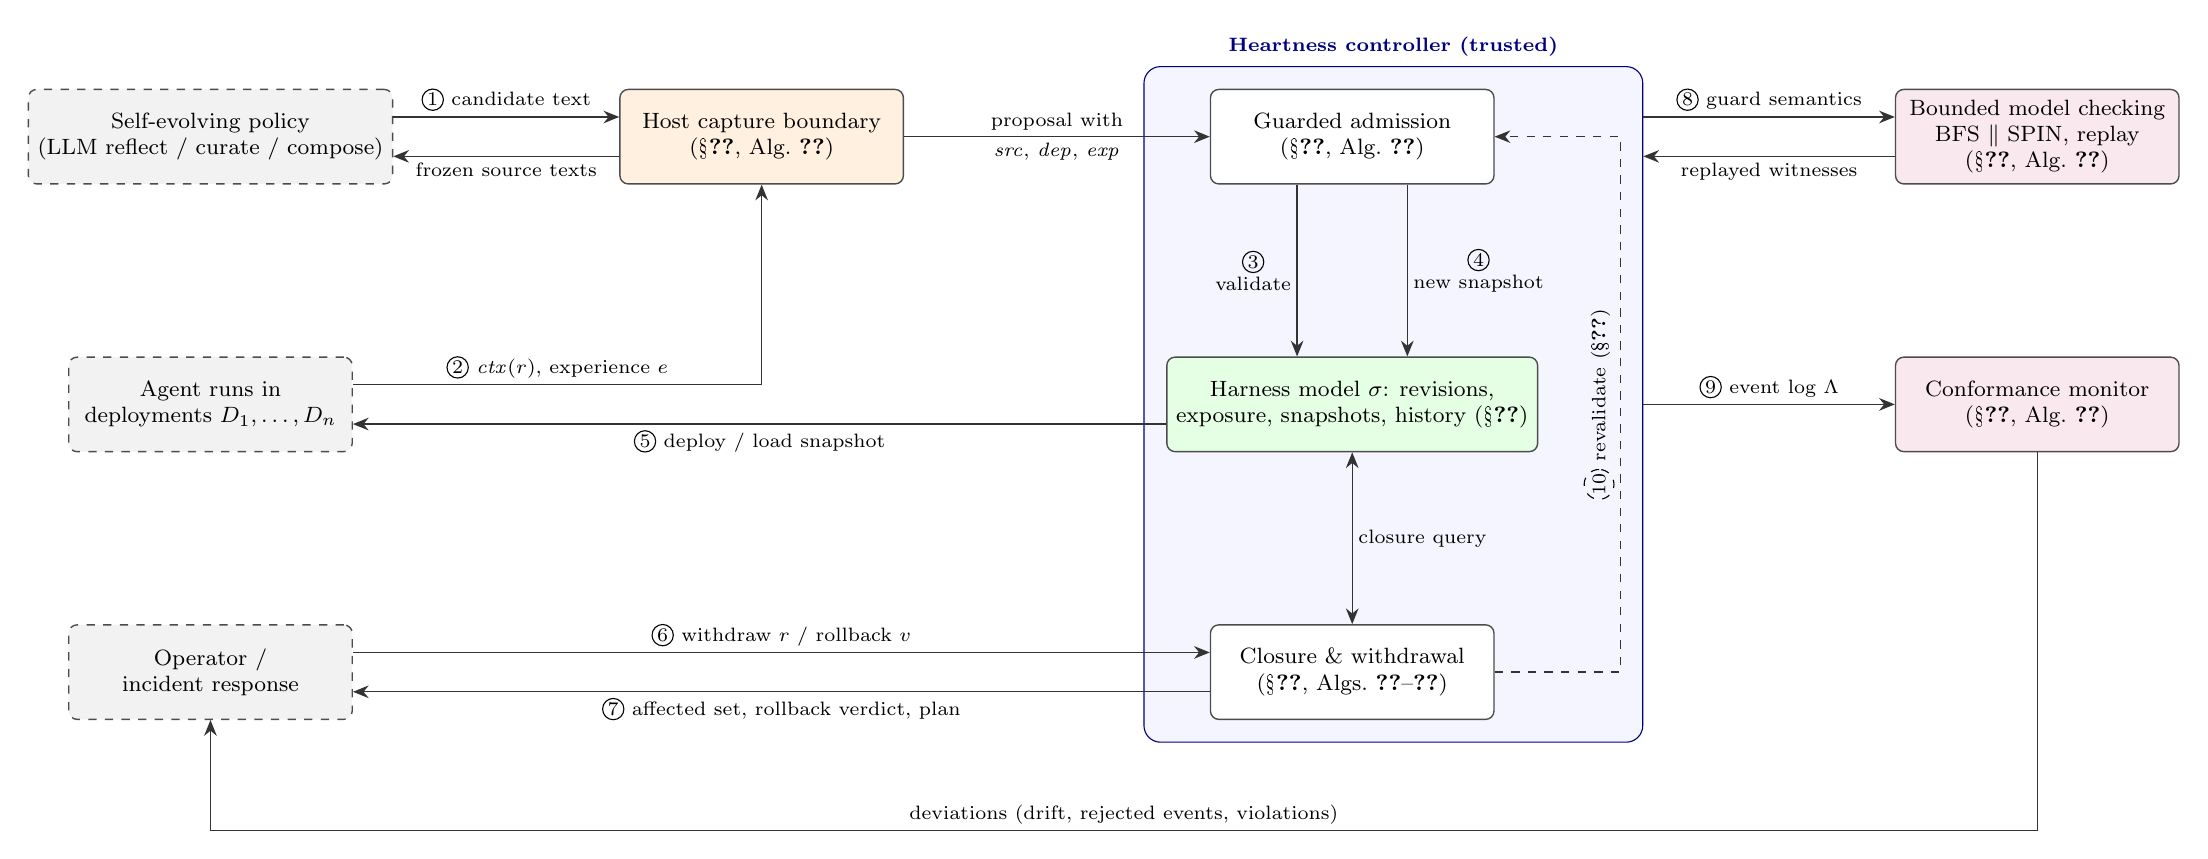
\begin{tikzpicture}[
  font=\footnotesize, >={Stealth[length=2mm,width=1.6mm]}, line width=0.5pt,
  comp/.style={draw=black!70, rounded corners=3pt, align=center, minimum height=12mm, minimum width=36mm, fill=white},
  ext/.style={comp, dashed, fill=gray!10},
  grp/.style={draw=blue!50!black, rounded corners=6pt, inner sep=8pt, fill=blue!4},
  lab/.style={font=\scriptsize, align=center, inner sep=2pt},
  flow/.style={->, draw=black!80},
  back/.style={->, draw=black!80, dashed}]
% ---- grid: columns x = 0, 7, 14.5, 23 ; rows y = 0, -3.4, -6.8
\node[ext] (policy) at (0,0) {Self-evolving policy\\(LLM reflect / curate / compose)};
\node[ext] (runs) at (0,-3.4) {Agent runs in\\deployments $D_1,\dots,D_n$};
\node[ext] (op) at (0,-6.8) {Operator /\\incident response};
\node[comp, fill=orange!12] (cap) at (7,0) {Host capture boundary\\(\S\ref{sec:capture}, Alg.~\ref{alg:capture})};
\node[comp] (adm) at (14.5,0) {Guarded admission\\(\S\ref{sec:admission}, Alg.~\ref{alg:admit})};
\node[comp, fill=green!10] (store) at (14.5,-3.4) {Harness model $\sigma$: revisions,\\exposure, snapshots, history (\S\ref{sec:metamodel})};
\node[comp] (wd) at (14.5,-6.8) {Closure \& withdrawal\\(\S\ref{sec:withdrawal}, Algs.~\ref{alg:closure}--\ref{alg:withdraw})};
\coordinate (rv) at ([xshift=16mm]wd.east);
\begin{scope}[on background layer]
\node[grp, fit=(adm)(store)(wd)(rv), label={[font=\scriptsize\bfseries,text=blue!50!black]above:\sys{} controller (trusted)}] (ctrl) {};
\end{scope}
\node[comp, fill=purple!9] (mc) at (23.2,0) {Bounded model checking\\BFS $\parallel$ SPIN, replay\\(\S\ref{sec:checking}, Alg.~\ref{alg:check})};
\node[comp, fill=purple!9] (mon) at (23.2,-3.4) {Conformance monitor\\(\S\ref{sec:monitor}, Alg.~\ref{alg:monitor})};
% 1: policy <-> capture (two straight parallel lines)
\draw[flow] ([yshift=2.5mm]policy.east) -- node[lab, above]{\circled{1} candidate text} ([yshift=2.5mm]cap.west);
\draw[flow] ([yshift=-2.5mm]cap.west) -- node[lab, below]{frozen source texts} ([yshift=-2.5mm]policy.east);
% capture -> admission
\draw[flow] (cap.east) -- node[lab, above]{proposal with} node[lab, below]{$\src$, $\dep$, $\expr$} (adm.west);
% 2: runs -> capture (orthogonal)
\coordinate (c2) at ([yshift=2.5mm]runs.east -| cap.south);
\draw[flow] ([yshift=2.5mm]runs.east) -- node[lab, above]{\circled{2} $\ctx(r)$, experience $e$} (c2) -- (cap.south);
% 5: model -> runs (straight)
\draw[flow] ([yshift=-2.5mm]store.west) -- node[lab, below]{\circled{5} deploy / load snapshot} ([yshift=-2.5mm]runs.east);
% 3,4: admission <-> model
\draw[flow] ([xshift=-7mm]adm.south) -- node[lab, left]{\circled{3}\\validate} ([xshift=-7mm]store.north);
\draw[flow] ([xshift=7mm]adm.south) -- node[lab, right]{\circled{4}\\new snapshot} ([xshift=7mm]store.north);
% model <-> withdrawal
\draw[<->, draw=black!80] (store.south) -- node[lab, right]{closure query} (wd.north);
% 10: revalidation loop (orthogonal, dashed)
\coordinate (rvtop) at (rv |- adm.east);
\draw[back] (wd.east) -- (rv) -- node[lab, sloped, above]{\circled{10} revalidate (\S\ref{sec:revalidation})} (rvtop) -- (adm.east);
% 6,7: operator <-> withdrawal (straight)
\draw[flow] ([yshift=2.5mm]op.east) -- node[lab, above]{\circled{6} withdraw $r$ / rollback $v$} ([yshift=2.5mm]wd.west);
\draw[flow] ([yshift=-2.5mm]wd.west) -- node[lab, below]{\circled{7} affected set, rollback verdict, plan} ([yshift=-2.5mm]op.east);
% 8: controller <-> model checking (straight)
\draw[flow] ([yshift=2.5mm]ctrl.east |- adm.east) -- node[lab, above]{\circled{8} guard semantics} ([yshift=2.5mm]mc.west);
\draw[flow] ([yshift=-2.5mm]mc.west) -- node[lab, below]{replayed witnesses} ([yshift=-2.5mm]ctrl.east |- adm.east);
% 9: controller -> monitor (straight)
\draw[flow] (ctrl.east |- mon.west) -- node[lab, above]{\circled{9} event log $\Lambda$} (mon.west);
% monitor -> operator (orthogonal, below everything)
\coordinate (bot) at ($(wd.south)+(0,-14mm)$);
\draw[flow] (mon.south) -- (mon.south |- bot) -- node[lab, above]{deviations (drift, rejected events, violations)} (op.south |- bot) -- (op.south);
\end{tikzpicture}}
\caption{Overview of \sys{}. Dashed boxes are untrusted or external; the shaded group is the trusted controller. Numbered arrows: \circled{1}~the policy returns only candidate text, \circled{2}~the host records each run's loaded context and resulting experience, \circled{3}--\circled{4}~admission validates the exact candidate against the current snapshot and installs a new immutable snapshot, \circled{5}~deployments load snapshots, \circled{6}--\circled{7}~withdrawal and rollback requests are answered with the affected set and an admissibility verdict, \circled{8}~a finite projection of the guards is model checked and witnesses are replayed on the implementation, \circled{9}~the event log is replayed by the conformance monitor, \circled{10}~revalidation re-admits screened members of the closure as fresh revisions under an attestation.}
\label{fig:overview}
\end{figure*}

The design rests on three explicit assumptions that the evaluation probes rather than presumes: (A1)~persistent state changes only through the controller's API (direct file edits are outside the model and are detected only if observed, Section~\ref{sec:monitor}); (A2)~the host, not the policy, records exposure, so exposure is complete for the inputs the host itself supplies but not for ambient inputs it does not mediate; (A3)~admissions are serialized against snapshot stamps (optimistic concurrency), and deployments are connected when withdrawn.

\subsection{Harness Metamodel and Lifecycle State}\label{sec:metamodel}
\emph{Motivation.} The queries in Section~\ref{sec:background} fail when relationships live only in file contents or in an informal log. The metamodel turns every relationship needed to answer them into a typed, immutable reference.

\emph{Design.} The metamodel (Definition~8) has classes Experience, ArtifactRevision (one tagged class for the seven artifact kinds and the attestations of Section~\ref{sec:revalidation}), Proposal, ValidationRecord, HarnessVersion, ExternalEffect, and Event, plus the relations \emph{motivatedBy}, \emph{derivedFrom}$(\mathit{kind})$, \emph{dependsOn}, \emph{replaces}, \emph{loadedContext}, and deployment membership. Revisions are content-addressed (SHA-256 of a canonical serialization), so a snapshot fixes both identities and contents. The state also holds the sets $W$ of withdrawn and $K$ of quarantined revisions and the set $\Theta$ of experiences withdrawn as evidence. The \emph{forbidden roots} are $F=W\cup K\cup\{b\mid\expr(b)\cap\Theta\neq\emptyset\}$; P2 and P8 forbid their whole closure $\Cl(F)$. We call the approach model-driven in the models@run.time sense~\cite{blair2009modelsruntime}: the metamodel is the runtime representation that every operator reads and writes, P1--P10 are invariants over its instances, the Promela model checked in Section~\ref{sec:checking} is generated from a projection of the operator semantics, and the conformance monitor replays the event log through the same operators; we do not use a metamodelling workbench. Lifecycle status is \emph{derived}, not stored: a revision can be historically accepted and currently suspended. Every operator either applies atomically and appends a hash-chained event to $\Lambda$, or is rejected and leaves $\sigma$ unchanged. Table~\ref{tab:props} lists the ten safety properties the controller maintains; all have the form $\mathbf{G}\,\varphi$.

\begin{table}[!t]
\caption{Safety properties maintained by \sys{} and the evidence used for each. ``Proj.'' = checked on the finite projection by both BFS and SPIN.}\label{tab:props}
\centering\footnotesize
\begin{tabular}{@{}p{0.06\columnwidth}p{0.58\columnwidth}p{0.24\columnwidth}@{}}
\toprule
ID & Predicate & Evidence \\
\midrule
P1 & every revision reaches an experience or an authorized seed via $\src$ & guard, audit, tests\\
P2 & $\Act\cap\Cl(F)=\emptyset$ & guard, audit, Proj.\\
P3 & active and deployed sets are contract-consistent & guard, audit, Proj.\\
P4 & accepted/loaded content equals validated/snapshot content & digest guard, Proj.\\
P5 & rollback restores the exact recorded set; effects are never removed & audit, tests\\
P6 & derivation endpoints exist; derivation graph is acyclic & guard, audit\\
P7 & history and revision identities are append-only & transition audit\\
P8 & no registered deployment contains $\Cl(F)$ & suspension, Proj.\\
P9 & an accepted proposal's base is the current snapshot & stamp guard, Proj.\\
P10 & event chain and observed digests agree with replay & monitor\\
\bottomrule
\end{tabular}
\end{table}

\emph{Running example.} After task~12 the model contains $m_0,\dots,m_{11}$, $k_0,k_1$, $p^{1}_{0},p^{1}_{12},p^{2}_{0},p^{2}_{12}$; $k_1$ has $\src=\{m_6,m_7,m_9\}$ (abbreviated), $p^{1}_{12}$ has $\src=\{p^{1}_{0},k_0,k_1\}$, $\dep=\{k_0,k_1\}$ and \emph{replaces} $p^{1}_{0}$; $\Dpl(D_1)=\{p^{1}_{12},k_0,k_1\}$; run $r_8$ has $\ctx(r_8)=\{p^{1}_{0},m_7,\ldots\}$ and produced $e_8$, which motivates $m_8$.

\emph{Assumptions and limits.} The metamodel captures declared structure only; it does not interpret natural-language content, and contracts are syntactic (Definition~7).

\subsection{Host-Side Exposure Capture}\label{sec:capture}
\emph{Motivation.} Provenance cannot be recovered after the fact from LLM output (Section~\ref{sec:bg-prov}); it must be recorded where inputs are assembled. Recording synthesis inputs alone is also insufficient: the running example shows that a faulty lesson can re-enter memory through the agent's behaviour ($m_7\rightsquigarrow m_8$).

\emph{Design.} The host performs two recordings (Algorithm~\ref{alg:capture}). Before every agent run it records the exact revisions placed in the context ($\textsc{Load}$, line~3); the controller rejects a context containing revisions that are neither active nor deployed. Before every generation step it freezes the selected source revisions and their texts, invokes the policy, and attaches the frozen identities to the proposal itself (lines~7--10). The policy never names its own sources. EME edges are then \emph{derived}: an artifact motivated by experience $e$ is exposed to every revision in $\ctx(\run(e))$.

\begin{algorithm}[!t]
\caption{Host-side exposure capture}\label{alg:capture}
\begin{algorithmic}[1]
\Procedure{RunTask}{$d$, task $t$}
  \State $C \gets$ \Call{AssembleContext}{$d,t$} \Comment{profile, skills, memories}
  \State \Call{Apply}{$\textsc{Load}(r, C)$}
  \State $o \gets$ execute agent on $t$ with $C$; \Call{Apply}{$\textsc{Experience}(e,t,r,o)$}
  \State \Return $e$
\EndProcedure
\Procedure{Generate}{policy $\pi$, sources $S$, experiences $E$, kind $\kappa$}
  \State $T \gets [\mathit{text}(s) \mid s\in S]$ \Comment{frozen before $\pi$ runs}
  \State $y \gets \pi(T, E)$ \Comment{untrusted text only}
  \State $a \gets \langle \mathit{fresh}, \kappa, y, \src{=}S, \expr{=}E\rangle$
  \State \Return \Call{Admit}{$a$} \Comment{Algorithm~\ref{alg:admit}}
\EndProcedure
\end{algorithmic}
\end{algorithm}

\emph{Running example.} For task~9 (run $r_8$), \textsc{AssembleContext} retrieves $p^{1}_{0}$, the most relevant skill $k_0$ and the three memories most similar to the task, including $m_7$; \textsc{Load}$(r_8,\{p^{1}_{0},k_0,m_5,m_6,m_7\})$ is recorded before the run produces its experience (\textsc{Load} is rejected for a run that already has one). The reflection that produces $m_8$ receives $e_8$ and two retrieved lessons, so $m_8$ gets $\src=\{m_5,m_6\}$ and $\expr=\{e_8\}$; the EME edge $m_7\rightsquigarrow m_8$ follows from $\ctx(r_8)$ without any action by the policy.

\emph{Assumptions, limits, cost.} Capture is complete only for inputs the host mediates (A2): a tool result that quotes an artifact, or the model's parametric knowledge, are not captured. Capture costs one set copy per run and per generation, linear in context size.

\subsection{Guarded Admission}\label{sec:admission}
\emph{Motivation.} A self-evolving loop proposes changes continuously; without a gate, a candidate can be modified after validation, validated against a stale snapshot, or admitted while it inherits from withdrawn state.

\emph{Design.} Admission (Algorithm~\ref{alg:admit}) has three operators. \textsc{Propose} checks freshness, typed kinds, known sources, dependencies and experiences (P1, P6) and stamps the proposal with the current snapshot as its base. \textsc{Validate} binds a Boolean outcome to the candidate's content digest and base; validation itself is pluggable (tests, reviewers, LLM judges). \textsc{Accept} requires a passed validation of the \emph{same} digest (P4), a base equal to the current snapshot (P9), and an admissible candidate active set: no member in the closure of withdrawn or quarantined revisions (P2) and contract consistency (P3). Success installs a new immutable snapshot; failure rolls back atomically.

\begin{algorithm}[!t]
\caption{Guarded admission (\textsc{Admit} = \textsc{Propose}, \textsc{Validate}, \textsc{Accept})}\label{alg:admit}
\begin{algorithmic}[1]
\Procedure{Propose}{candidate $a$}
  \State \textbf{require} $\src(a)\cup\dep(a)\subseteq\mathcal{A}$, $\expr(a)\subseteq\mathcal{E}$, $\src(a)\cup\expr(a)\neq\emptyset$ or seed \Comment{P1, P6}
  \State \Return $q\gets\langle a, \mathit{base}{=}|\mathit{Ver}|{-}1\rangle$ \Comment{stamp current snapshot}
\EndProcedure
\Procedure{Validate}{$q$}
  \State \Return $v\gets\langle q, \mathit{hash}(q.a), \mathit{check}(q.a)\rangle$ \Comment{pluggable check}
\EndProcedure
\Procedure{Accept}{$q$, $v$} \Comment{possibly after other admissions}
  \State \textbf{require} $v.\mathit{passed}\wedge v.\mathit{hash}=\mathit{hash}(q.a)$ \Comment{P4}
  \State \textbf{require} $q.\mathit{base}=|\mathit{Ver}|-1$ \Comment{P9: no admission since Propose}
  \State $S\gets(\Act\cup\{q.a\})\setminus\mathit{replaces}(q.a)$
  \State \textbf{require} $S\cap\Cl(F)=\emptyset$\label{line:p2} \Comment{P2; $\Cl$ over $\mathcal{A}\cup\{q.a\}$}
  \State \textbf{require} \Call{Consistent}{$S$} \Comment{P3}
  \State $\Act\gets S$; append snapshot $\langle S, \{(x,\mathit{hash}(x))\}_{x\in S}\rangle$
\EndProcedure
\end{algorithmic}
\end{algorithm}

\emph{Running example.} The composition step proposes $p^{1}_{12}$ with base~$v$, replacing $p^{1}_{0}$. If another admission (say $k_1$) lands in between, the base is stale and \textsc{Accept} rejects $p^{1}_{12}$ (P9); the host re-proposes against the new snapshot. Once $m_7$ is withdrawn, any later proposal that merges $m_8$ is rejected by line~\ref{line:p2}: the closure is computed over the stored revisions \emph{plus the candidate}, and the candidate is a child of $m_8\in\Cl(\{m_7\})$, so it lies in the closure itself. The same holds for a candidate motivated by an experience whose run loaded $m_7$ before the withdrawal.

\emph{Assumptions and cost.} Line~\ref{line:p2} recomputes a closure, $O(|\mathcal{A}|+|{\rightsquigarrow}|)$ per acceptance; Section~\ref{sec:rq3} measures this cost. Validation quality is outside the controller: a passing but wrong validator admits wrong content, which is exactly the situation withdrawal must then repair.

\subsection{Exposure Closure, Withdrawal, and Rollback}\label{sec:withdrawal}
\emph{Motivation.} Once a revision is known to be faulty, every revision that inherits from it and every deployment that loads such a revision must be found and contained; restoring an old snapshot must not silently reactivate withdrawn lineage.

\emph{Design.} Algorithm~\ref{alg:closure} computes $\Cl(R)$ by breadth-first search over three successor relations: derivation children, dependency consumers, and EME children, the last obtained by joining each revision's experiences with the contexts of the runs that produced them. Algorithm~\ref{alg:withdraw} withdraws a root: it records the root in $W$, quarantines every other revision of the closure in $K$, removes the closure from $\Act$ and from every deployment (P2, P8), and appends a snapshot; nothing is deleted. The part of the closure that was in use, $Z\cap(\Act\cup\bigcup_d\Dpl(d))$, is the affected set of Definition~5 that is reported to the operator (Fig.~\ref{fig:overview}, \circled{7}). \textsc{Withdraw} also accepts an \emph{experience} $e$: it marks $e$ as tainted evidence, withdraws every revision whose motivation $\expr(\cdot)$ contains $e$ together with its closure, and makes every \emph{future} revision motivated by $e$ a forbidden root, so that a policy that re-reads its experience pool cannot re-learn the same lesson from the same corrupted feedback (P2). Re-learning from \emph{new} evidence, such as a second corrupted message, is outside what any lineage-based guard can prevent. \textsc{Rollback} to snapshot $v$ is admissible only if the target set passes the same checks as admission; otherwise it is rejected and the operator receives the most recent admissible snapshot (\textsc{LastGood}) and the list of external effects that rollback cannot reverse.

\begin{algorithm}[!t]
\caption{Exposure closure $\Cl(R)$}\label{alg:closure}
\begin{algorithmic}[1]
\State $\mathit{child}[x]\gets\{b\mid x\in\src(b)\}$; $\mathit{cons}[x]\gets\{b\mid x\in\dep(b)\}$
\State $\mathit{eme}[x]\gets\{b\mid \exists e\in\expr(b): x\in\ctx(\run(e))\}$
\State $S\gets R$; $Q\gets R$
\While{$Q\neq\emptyset$}
  \State $x\gets$ \Call{Pop}{$Q$}
  \For{$b\in\mathit{child}[x]\cup\mathit{cons}[x]\cup\mathit{eme}[x]\setminus S$}
    \State $S\gets S\cup\{b\}$; \Call{Push}{$Q,b$}
  \EndFor
\EndWhile
\State \Return $S$
\end{algorithmic}
\end{algorithm}

\begin{algorithm}[!t]
\caption{Withdrawal and rollback admissibility}\label{alg:withdraw}
\begin{algorithmic}[1]
\Procedure{Withdraw}{$r$} \Comment{$r$ a revision or an experience}
  \If{$r\in\mathcal{E}$} $\Theta\gets\Theta\cup\{r\}$; $R\gets\{b\mid r\in\expr(b)\}$ \Else\ $R\gets\{r\}$ \EndIf
  \State $Z\gets\Cl(R)$; $W\gets W\cup R$; $K\gets K\cup(Z\setminus R)$
  \State $\Act\gets\Act\setminus Z$
  \ForAll{deployments $d$} $\Dpl(d)\gets\Dpl(d)\setminus Z$ \EndFor
  \State append snapshot; \Return $Z$ and external effects $X$ (not reversed)
\EndProcedure
\Procedure{Rollback}{$v$}
  \State $S\gets\mathit{Ver}[v].\mathit{active}$
  \If{$S\cap\Cl(F)\neq\emptyset\vee\neg$\Call{Consistent}{$S$}}
    \State \textbf{reject}; \Return \Call{LastGood}{}, $X$
  \EndIf
  \State $\Act\gets S$; append snapshot ``rollback:$v$''
\EndProcedure
\end{algorithmic}
\end{algorithm}

\emph{Running example.} \textsc{Withdraw}$(m_7)$ visits $m_7\to k_1$ (child), $m_7\to m_8$ (EME), $k_1\to p^{1}_{12},p^{2}_{12}$ (child and consumer), and any revision later exposed to these; both deployments lose $k_1$ and their rewritten profiles and keep $k_0$. Withdrawal never re-activates the replaced base profiles $p^{1}_{0},p^{2}_{0}$ by itself; the operator restores them explicitly, by redeploying them or by rolling back to an admissible snapshot. A rollback to the snapshot installed right after $k_1$ is rejected because that snapshot contains $k_1\in K$; \textsc{LastGood} returns the most recent snapshot disjoint from the closure. Rollback changes $\Act$ only; deployments change through \textsc{Deploy}, so a rollback reaches agents only when it is redeployed. The phrase ``any revision later exposed to these'' dominates the cost in practice: because every run after task~12 loads its deployment's rewritten profile, every memory written after that point is EME-exposed to $p^{1}_{12}$ or $p^{2}_{12}$ and joins the closure; only memories written between the fault and the rewrite by runs that never loaded $m_7$ or its descendants are spared. Section~\ref{sec:rq1-live} measures exactly this effect.

\emph{Design rationale and limits.} Closure deliberately over-approximates: $k_1$ is suspended although only one of its three sources was faulty, and it would be suspended even if its text had dropped the faulty advice. Revisions that are not exposed to $m_7$, such as $m_9$ itself, stay active. Proposition~\ref{prop:cut} states the bound this over-approximation obeys. Quarantine is permanent; suspended state returns to use only through closure-bounded revalidation (Section~\ref{sec:revalidation}) or fresh lineage. The BFS is linear in the number of revisions and exposure edges.

\begin{proposition}[Closure is bounded by a time cut]\label{prop:cut}
Let $t(b)$ be the position in $\Lambda$ of the event that accepted revision $b$ ($t(b)=0$ for seeds). For every root set $R$, $\Cl(R)\subseteq\{b\in\mathcal{A}\mid t(b)\ge\min_{r\in R}t(r)\}$.
\end{proposition}
\begin{IEEEproof}
Every edge $x\rightsquigarrow b$ has $t(x)<t(b)$; the EME case relies on the \textsc{Load} precondition that a run's context is recorded before the run produces an experience. For synthesis and dependency edges, \textsc{Propose} requires $x\in\mathcal{A}$, so $x$ was accepted before $b$ was proposed. For an EME edge, $x\in\ctx(\run(e))$ with $e\in\expr(b)$: \textsc{Load} admits only active or deployed revisions into a context, the run precedes its experience, and \textsc{Propose} requires $e\in\mathcal{E}$. Hence every path from a root to $b$ is increasing in $t$.
\end{IEEEproof}
\noindent Consequently, withdrawal never suspends more than restoring the last snapshot before the earliest root (a \emph{time cut}), and it suspends exactly the same set as that cut when every revision accepted after the root is exposed to it. The time-cut baseline of the evaluation cuts before the corrupted \emph{experience}, which precedes the root's acceptance, so it suspends at least as much and the bound holds for it as well. How far closure stays below the time cut is therefore determined by the exposure structure of the self-evolving policy, which the evaluation measures (Section~\ref{sec:rq1-live}). Closure differs from the time cut in two respects: it keeps later work that was not exposed, and it is enforced on future admissions, rollbacks and deployments rather than applied once. Both compute from the same input, since the root's acceptance time is in $\Lambda$; reaching every deployment is a requirement on any remedy in a multi-deployment harness, which \sys{} satisfies by construction (P8) and a rollback satisfies only if it is redeployed.

\subsection{Closure-Bounded Revalidation}\label{sec:revalidation}
\emph{Motivation.} Proposition~\ref{prop:cut} bounds the over-approximation but does not remove it: when a policy exposes most later revisions to the root, withdrawal suspends most learned state. Detectors that judge content are more precise but may miss contaminated revisions, and applied to the whole state they can also flag revisions that have nothing to do with the root.

\emph{Design.} Revalidation uses the closure as the \emph{candidate set} and a screen only to give members back (Algorithm~\ref{alg:reval}). A pluggable screen (an LLM judge or a similarity threshold, relative to the text of the withdrawn roots) decides for each quarantined member whether it is free of the faulty content. Candidates are the members of the affected set (Definition~5) before the withdrawal, other than the roots, that the screen clears; because the affected set contains only revisions in use (active or deployed), a revision that a later version had already replaced does not return beside its successor. If any candidate is admissible, revalidation first admits one \emph{attestation} revision $\alpha=\langle R,\phi,C\rangle$, a host-authorized seed. Each cleared member $x$ is then re-admitted, in history order, as a fresh revision $x'$ with the same text and contract. Its lineage is $x$'s lineage with the withdrawn part replaced by $\alpha$: its sources are $\alpha$, the sources of $x$ outside $\Cl(F)$ (active or not), and the re-admitted copies of those that were cleared; it keeps the experiences of $x$ whose run context avoided $\Cl(F)$; every source or experience that cannot be kept is replaced by its \emph{clean frontier}: the nearest ancestor revisions outside $\Cl(F)$, active or not, and the clean experiences that motivated dropped intermediates; and its dependencies are $\dep(x)$ with every quarantined dependency replaced by its re-admitted copy. A later withdrawal of any clean ancestor of $x$ therefore still reaches $x'$. A member with a dependency that is neither active nor re-admitted is rejected, as admission would reject it (P3): a profile returns only if the skills it depends on do. Admitted copies are redeployed to the deployments that held the original before the withdrawal ($\Dpl_{\mathrm{b}}$). The original $x$ stays quarantined and the history keeps both. Because every source, experience context and dependency of $x'$ lies outside $\Cl(F)$, so does $x'$, and P2 holds; because it derives from $\alpha$, withdrawing the attestation (for example, when the screen is found faulty) suspends every re-admission through the ordinary closure. Revalidation is thus a composition of existing operators and adds no semantics; the implementation (\texttt{heartness.revalidation}) executes it with \textsc{Propose}, \textsc{Validate}, \textsc{Accept} and \textsc{Deploy}.

\begin{algorithm}[!t]
\caption{Closure-bounded revalidation}\label{alg:reval}
\begin{algorithmic}[1]
\Require roots $R$, screen $\phi$; $\Act_{\mathrm{b}}$, $\Dpl_{\mathrm{b}}$: active set and deployments before withdrawal
\State $C\gets\{x\in \Cl(R)\setminus R\mid x\in\Act_{\mathrm{b}}\cup\bigcup_d\Dpl_{\mathrm{b}}(d),\ \phi(\mathit{text}(x),\mathit{text}(R))=\mathit{clean}\}$
\State $\nu\gets\emptyset$ \Comment{$\nu$: original $\mapsto$ copy}
\If{some $x\in C$ has all dependencies active or in $C$} \Call{Admit}{$\alpha$} with $\alpha=\langle R,\phi,C\rangle$ as authorized seed \EndIf
\ForAll{$x\in C$ in history order}
  \State $D\gets\{\nu(y)\text{ if }y\in\mathrm{dom}\,\nu\text{ else }y\mid y\in\dep(x)\}$
  \If{$D\subseteq\Act$} \Comment{else rejected (P3)}
    \State $S_x\gets\{\alpha\}\cup$ kept sources $\cup$ clean frontier of dropped sources and contexts
    \State $x'\gets$ copy of $x$ with $\src(x'){=}S_x$, $\dep(x'){=}D$, clean experiences
    \State \Call{Admit}{$x'$}; $\nu(x)\gets x'$
  \EndIf
\EndFor
\ForAll{$d$} \Call{Deploy}{$d$, $\Dpl(d)\cup\{\nu(x)\mid x\in\Dpl_{\mathrm{b}}(d)\cap\mathrm{dom}\,\nu\}$} \EndFor
\end{algorithmic}
\end{algorithm}

\emph{Running example.} After \textsc{Withdraw}$(m_7)$, the judge reads $k_1$, $p^{1}_{12}$, $p^{2}_{12}$ and $m_8$ against $m_7$. If $k_1$'s merged text had dropped the print instruction, the judge would clear it and $k_1'$ would be re-admitted and redeployed; $m_8$ and the profiles, which repeat the advice, stay quarantined. Had the judge cleared $p^{1}_{12}$ but not $k_1$, $p^{1}_{12}$ would be rejected, because it depends on $k_1$.

\emph{Limits.} Revalidation is only as good as its screen; a missed contaminated member returns to use, which the evaluation measures as residual contamination. It never re-admits revisions outside the closure and never needs to inspect them, so its cost is bounded by the affected set. In the live study we evaluate revalidation on the recorded final state in a separate process: the same planning function that the implementation executes (\texttt{heartness.revalidation.plan}) decides which cleared members are re-admitted, and a test checks on small fixtures that the plan equals the engine's execution. The plan checks only dependency availability; in the engine every copy also passes the ordinary admission guards, which could reject it, but in the live records they cannot bind: a copy's sources, experience contexts and dependencies are by construction outside $\Cl(F)$, its content hash is the one validated, and contracts are those of the original.

\subsection{Bounded Model Checking and Implementation Correspondence}\label{sec:checking}
\emph{Motivation.} The guards interact: deployment replacement, repeated withdrawal and rollback all change snapshots and base stamps. Testing individual operations does not show that no \emph{sequence} reaches a state violating P2--P9.

\emph{Design.} We define a finite projection of the lifecycle with $n\le 8$ revision identities, a static derivation/dependency topology (chain, star, or independent), Boolean validation, and the operators Propose, Validate, Accept, Withdraw, Deploy and Rollback. The projection is encoded twice, independently: as an explicit breadth-first search in Python, which yields shortest counterexamples, and as a Promela model checked by SPIN 6.5.2~\cite{holzmann1997spin,spin}. Algorithm~\ref{alg:check} runs both on the reference guards and on seeded \emph{guard mutants} (each removing one guard), compares verdicts, replays each witness on the projection and on the real engine with the same guard disabled, and checks minimality by re-running at depth $\ell-1$. A separate experiment maps every successor of small reference states between the engine and the projection and compares enabled operations and mapped state fields.

\begin{algorithm}[!t]
\caption{Bounded checking and witness replay}\label{alg:check}
\begin{algorithmic}[1]
\Require scope $(n,\mathit{topology},\mathit{depth})$, mutant $\mu$ (or none)
\State $(\mathit{safe}_B,w)\gets$ \Call{BFS}{$\mathit{init}(n)$, $\mathit{step}_\mu$, $\mathit{depth}$}
\State $P\gets$ \Call{Promela}{$n,\mathit{topology},\mu$}; $\mathit{safe}_S\gets$ \Call{SPIN}{$P$}
\State \textbf{record} $\mathit{agree}\gets(\mathit{safe}_B=\mathit{safe}_S)$
\If{$\neg\mathit{safe}_B$}
  \State \textbf{record} \Call{ReplayProjection}{$w$}, \Call{BFS}{$\ldots,|w|{-}1$} is safe
  \State \textbf{record} violations of \Call{ReplayEngine}{$w$, disabled${=}\mu$}
\EndIf
\end{algorithmic}
\end{algorithm}

\emph{Running example.} With three identities in a chain ($m_7\to k_1\to p_{12}$) and the suspension guard for P2 removed, BFS returns the 7-operation witness Propose, Validate, Accept $m_7$; Propose, Validate, Accept $k_1$; Withdraw $m_7$. Withdrawal then removes only $m_7$, so $k_1$ stays active although its source is withdrawn (P2) and although it depends on a revision that is no longer active (P3). SPIN agrees, no shorter witness exists, and replaying the sequence on the engine with the same guard removed produces audit violations P2 and P3.

\emph{Limits.} Agreement between two encodings of the same projection is cross-validation, not a refinement proof; the projection omits text, reduces contracts to the presence of dependencies, and omits effects, EME edges, multiple deployment identities, experience withdrawal and revalidation; the mutation campaign also does not cover the last two, which are covered by unit tests. Proposition~\ref{prop:inv} covers what the projection omits, for P2 and P8.

\begin{proposition}[Suspension invariant]\label{prop:inv}
With the forbidden roots $F$ of Section~\ref{sec:metamodel}, let $I(\sigma)$ be $\Act\cap\Cl(F)=\emptyset\wedge\forall d:\Dpl(d)\cap\Cl(F)=\emptyset$ (P2 and P8), with $\Cl$ over all exposure edges including EME. If $I(\sigma)$ holds and $\sigma\xrightarrow{op}\sigma'$ is any successful operator of the engine, then $I(\sigma')$ holds. The proposition concerns the \emph{recorded} closure: it says that nothing recorded as exposed to withdrawn lineage is in use, not that all contaminated content is.
\end{proposition}
\begin{IEEEproof}[Proof sketch]
By cases. \textsc{Experience}, \textsc{Propose}, \textsc{Validate}, \textsc{Load} and \textsc{Effect} leave $\Act$, $\Dpl$, $W$, $K$, $\Theta$ unchanged and add no edge between stored revisions: stored revisions are immutable and cannot cite an experience created after them, and \textsc{Load} is rejected for a run that has already produced an experience, so a late context record cannot add EME edges into accepted revisions. \textsc{Accept} adds one revision $a$ and edges only \emph{into} $a$, so $\Cl(F)$ grows at most by $a$; the guard rejects the operation if the candidate set meets the closure computed with $a$ included. \textsc{Retire} only shrinks $\Act$ and $\Dpl$. \textsc{Withdraw}$(r)$ and \textsc{Quarantine}$(r)$ remove $\Cl(\{r\})$ from $\Act$ and every $\Dpl(d)$, and $\Cl(F\cup\{r\})=\Cl(F)\cup\Cl(\{r\})$; withdrawing an experience $e$ applies this to every revision motivated by $e$, and any later revision motivated by $e$ is in $F$ and is rejected by the \textsc{Accept} guard. \textsc{Rollback} and \textsc{Deploy} install a set only after the same admissibility check.
\end{IEEEproof}
\noindent The proposition is a hand proof over the engine's operator semantics, not a mechanized one; the bounded checks and the mutation tests (Section~\ref{sec:impl}) give independent evidence that the implementation follows it. Scopes are small; the state space grows exponentially with $n$ (Section~\ref{sec:rq3}).

\subsection{Runtime Conformance Monitor}\label{sec:monitor}
\emph{Motivation.} Model checking speaks about the model; the deployed harness can still drift, for example when a file is edited outside the API.

\emph{Design.} Algorithm~\ref{alg:monitor} replays a logged event sequence through a fresh reference engine, compares each recomputed state digest with the observed one, and evaluates the audit predicates P1--P10 on every transition. It fails closed: after a rejected event there is no synchronized reference, so monitoring stops and reports.

\begin{algorithm}[!t]
\caption{Conformance monitor}\label{alg:monitor}
\begin{algorithmic}[1]
\Require logged events $\langle(op_i,\mathit{args}_i,h_i)\rangle_i$
\State $\sigma\gets\sigma_0$; $D\gets[\,]$
\For{$i=1,\dots$}
  \State $\sigma'\gets$ \Call{Apply}{$op_i,\mathit{args}_i$} \textbf{or} append (\emph{rejected}, $i$) to $D$ and \textbf{stop}
  \If{$h_i\neq\bot\wedge h_i\neq\mathit{hash}(\sigma')$} append (\emph{drift}, $i$) \EndIf
  \State append violations of P1--P10 on $(\sigma,\sigma')$; $\sigma\gets\sigma'$
\EndFor
\State \Return $D$
\end{algorithmic}
\end{algorithm}

\emph{Running example.} If someone edits the file of $k_1$ in $D_2$ after withdrawal, the next logged \textsc{Load} carries a digest that differs from replay and is reported as drift. If the agent sent an e-mail under $p^{2}_{12}$ and the host never logged it, nothing is reported: unlogged actions are invisible to any log-based monitor.

%% EVALUATION
\section{Evaluation}\label{sec:eval}
The evaluation answers the three research questions stated in Section~\ref{sec:intro}. RQ1 concerns containment effectiveness, RQ2 the assurance provided by the guards and the bounded checking, and RQ3 cost and the limits of runtime conformance.

\subsection{Implementation}\label{sec:impl}
\sys{} is implemented in Python~3.12 (\SrcLines{} lines in \texttt{src/heartness}): the metamodel as frozen dataclasses with canonical SHA-256 digests (\texttt{model.py}), transactional operators with atomic rollback (\texttt{engine.py}, Algorithms~\ref{alg:admit} and \ref{alg:withdraw}), the closure including EME edges (\texttt{graph.py}, Algorithm~\ref{alg:closure}), the host capture adapter (\texttt{capture.py}, Algorithm~\ref{alg:capture}), the audit predicates P1--P10 (\texttt{properties.py}), closure-bounded revalidation (\texttt{revalidation.py}, Algorithm~\ref{alg:reval}), the conformance monitor (\texttt{monitor.py}, Algorithm~\ref{alg:monitor}), and the finite projection with its BFS and Promela generator (\texttt{checker.py}, Algorithm~\ref{alg:check}). SPIN~6.5.2 is built from a pinned commit. A JSON command-line interface exposes withdrawal plans and rollback verdicts over saved event logs. Each guard can be disabled individually, which provides the mutants and ablations used below. The implementation has \TestCount{} tests with \LineCoverage\% statement and \BranchCoverage\% branch coverage, and strict \texttt{mypy}; \MutationKilled/\MutationTotal{} hand-seeded source mutants of the guards are killed by the test suite.

The live study (Section~\ref{sec:setup}) adds a self-evolving coding harness with its analysis and batch drivers (\LiveHarnessLines{} lines in \texttt{experiments/live}) whose every persistent write goes through the controller. It serves open-weight models through a private Ollama~0.32.14 server started inside each batch job, with temperature~0, fixed per-request seeds and a fixed 8{,}192-token context; every model response is cached by a digest of model, prompt and options, so each reported run can be replayed without a model server. The live study ran on the Fir cluster of the Digital Research Alliance of Canada, one job per cell on a 20\,GB slice of an NVIDIA \LiveGPU{}; the synthetic experiments, the model checking and the local pilot ran on one NVIDIA DGX Spark--class machine (GB10, 20 CPU cores, 121\,GB unified memory). The HPC pipeline (job graph, smoke test, audit and collection) is part of the replication package.

\subsection{Experimental Setup}\label{sec:setup}
\subsubsection{Subjects}
Table~\ref{tab:subjects} lists the three subjects and which RQs use them.

\emph{(S1) Live self-evolving harness.} We needed a setting where faulty state arises and spreads through real LLM generation, and where the damage can be measured independently of our own provenance records. We therefore implemented a self-evolving coding harness and evolved it on HumanEval+~\cite{chen2021codex,liu2023evalplus}, a widely used code-generation benchmark whose extended tests give an objective pass/fail signal. Of its 164 tasks, \LiveEvalTasks{} fixed held-out tasks measure behaviour and the remaining tasks supply the evolution stream (\LiveEvolveTasks{} tasks per run, shuffled per seed).\footnote{HumanEval/32 is excluded because its canonical solution fails its own HumanEval+ tests in our sandbox. All 163 remaining canonical solutions were re-validated in the batch environment before every campaign.} A run serves two deployments $D_1$ and $D_2$ and alternates tasks between them. Every task is solved from a context assembled by the host, its solution is tested, and the outcome and test feedback are recorded as an experience. How experiences become lasting state is the \emph{harness policy}, and we use two:
\begin{itemize}
\item \emph{ExpeL-style insights} (adapted from ExpeL~\cite{zhao2024expel} to single attempts; not an exact re-implementation). Every four tasks the model is shown the batch's attempts with their test feedback and the current insight list, and answers with ADD, EDIT, AGREE and REMOVE operations. Insights carry importance scores (ADD${}=2$, EDIT and AGREE ${+}1$, REMOVE ${-}1$; an insight at importance $\le 0$ is retired). $D_1$ loads all insights and $D_2$ the five most important, and every task context is the deployment's insight list. A new or edited insight records every insight shown to the extraction step as a source and the batch's experiences as its motivation. Importance scores are ranking metadata kept by the harness, not governed revisions; changing them changes which insights $D_2$ loads but not what any insight says.
\item \emph{Curation} (the running example, Section~\ref{sec:bg-example}). After every task the model writes a one-sentence memory from the experience, with the two most similar memories as sources; each context holds the deployment's profile, its two most relevant skills and the three most relevant memories; every six tasks the model merges recent memories into a skill; after tasks 12 and 24 each deployment's profile is rewritten from the current skills. A faulty lesson can therefore reach a profile in two synthesis hops, and a run that loads a faulty artifact can produce a new memory through its experience.
\end{itemize}
The two policies differ in exactly the structure that matters for containment: insight editing keeps one flat, heavily cross-sourced list, whereas curation builds a layered hierarchy (memory, skill, profile) with use dependencies.

In each \emph{faulty} run exactly one test-feedback message, at a seed-dependent position (task \LiveEFaultPositions{} for our seeds), is replaced by misleading grader feedback of one of three types: F1 \emph{print instead of return}, F2 \emph{stringify return values}, F3 \emph{use floor division}. All three are plausible misreadings of real test failures, and all three are wrong for HumanEval+. A paired \emph{clean} run with the same seed receives no corrupted feedback. The \emph{roots} of a faulty run are the revisions the controller recorded as motivated by the corrupted experience; they are known by construction and given to every remedy. Under curation this is the single memory written from that experience; under the ExpeL-style policy it is every insight the extraction step wrote from the batch containing it (\LiveERootsMean{} on average, at most \LiveERootsMax{}), of which typically at most one carries the faulty advice. Identifying the root is thus given to all remedies alike; we do not evaluate how an operator finds it. We used \LiveModels{} open-weight generators from five organizations that are common in code-generation studies: \texttt{qwen2.5-coder:7b}, \texttt{llama3.1:8b}, \texttt{deepseek-coder-v2:16b}, \texttt{gemma2:9b} and \texttt{granite3.3:8b}. For each policy, generator and reporting seed (\LiveSeeds{} seeds) we ran the three faulty runs and the clean run, \LiveTotalRuns{} runs in total. Thresholds were tuned beforehand on a separate local pilot (\PilotDevRuns{} development runs, Section~\ref{sec:baselines}) that is not part of the reported data.

\emph{(S2) Controlled synthetic benchmark.} Live runs give realistic content but no control over graph structure, and their ground truth is only as good as the content oracle. The synthetic benchmark (EvoTraceBench~1.1, \texttt{benchmark/}) generates provenance DAGs with seven artifact kinds, nine structural motif families (e.g., multi-source synthesis, adversarial lexical decoupling, dependency-only consumers, deployment-only membership), sizes 16--256 (up to 2{,}048 for scaling), controlled capture rates and lexical decoupling, with exact construction-time ground truth computed independently of \sys{}'s graph code. Hand-specified cases supply additional controls that do not depend on the generator.

\emph{(S3) Public skill-library replay.} To check that the model accepts a real third-party evolution artifact, we replay the \PublicRevisions{} revisions of Voyager's published skill library~\cite{wang2024voyager,voyagerrepo} as \PublicEvents{} controller events.

\emph{Compute platform.} The live study needs GPU inference for several open-weight models, so we prepared four Alliance Canada GPU clusters (Nibi, Narval, Fir, Rorqual) behind one submission and monitoring interface and ran an end-to-end smoke test (8 evolution tasks, one seed) on each. The smoke runs on Fir, Rorqual and Narval completed the full pipeline (setup, generation, oracle labelling, collection); the Nibi smoke run never started because its GPU nodes were unavailable. Smoke results were used only to find and fix deployment faults and are not reported as findings. We ran the reported study on one cluster (Fir) for four reasons. (i)~The platform is not an experimental factor: every compared condition is applied to the same recorded run, so a platform effect would shift all conditions alike. (ii)~Splitting the study would have introduced a confound, because the clusters differ in GPU model (H100, A100) and GPU kernels change low-order results even at temperature~0. (iii)~The software stack is pinned and recorded in every run record (inference-server version, model digests, checksummed benchmark files, code hash, cluster and GPU), so the setup can be repeated elsewhere. (iv)~Statistical power depends on faults, seeds and generators, not on the number of sites. The remaining limitation is stated in Section~\ref{sec:threats}.

\begin{table}[!t]
\caption{Subjects. S1 is generated by real LLM self-evolution; S2 has exact structural ground truth; S3 is a public evolution artifact.}\label{tab:subjects}
\centering\footnotesize
\begin{tabular}{@{}p{0.2\columnwidth}p{0.5\columnwidth}p{0.16\columnwidth}@{}}
\toprule
Subject & Size & RQs \\
\midrule
S1 live harness & \LiveTotalRuns{} runs (\LiveModels{} generators $\times$ \LivePolicies{} policies $\times$ \LiveSeeds{} seeds $\times$ (3 faults + clean)); \LiveEvalTasks{} held-out tasks $\times$ \LiveEvalConditions{} evaluated conditions per faulty run (\LiveConditions{} conditions in total); \LiveLLMCalls{} LLM calls & RQ1, RQ3 \\
S2 synthetic & \RawRecords{} raw records; \TraceCases{} traceability scenarios & RQ1, RQ2, RQ3 \\
S3 Voyager & \PublicRevisions{} skill revisions, \PublicEvents{} events & RQ3 \\
\bottomrule
\end{tabular}
\end{table}

\subsubsection{Baselines}\label{sec:baselines}
The baselines represent what a team can do today without \sys{}. All receive the same roots and act on the same final state. On S1 we name them R1--R4 and T, A; on S2 the corresponding structural baselines are B0--B3.
\begin{itemize}
\item \emph{R1 delete root}: remove the faulty memory, as a file-level revert or \texttt{git rm} would. On S2 the corresponding baseline (B0) recovers lineage from within-file history only.
\item \emph{R2 lexical recovery}: suspend artifacts whose TF-IDF cosine to the root reaches $\tau_t$, the classic IR traceability-recovery approach~\cite{antoniol2002}. On S2 (B1), chronological token Jaccard with a fixed threshold of 0.2.
\item \emph{R3 embedding recovery}: suspend artifacts whose \texttt{nomic-embed-text} embedding cosine to the root reaches $\tau_e$.
\item \emph{R4 LLM judge}: ask the generator model, for every live artifact, whether it repeats or relies on the root's (wrong) advice, a semantic content screen. The judge is shown the concatenated text of all roots of the run; under the ExpeL-style policy most roots are clean co-batched insights, which may lower its precision there.
\item \emph{T rollback before the fault}: restore the last snapshot before the corrupted experience, which suspends every revision created since. It needs the time of the fault, which the history provides for any known root, and by Proposition~\ref{prop:cut} it is the upper bound of the closure.
\item \emph{A reset learned state}: suspend every learned (non-seed) revision, i.e., return to the hand-written harness.
\item \emph{Capture-only provenance} (S2, B2): the recorded edges and the same closure, without admission, suspension or rollback semantics, representing PROV-style capture~\cite{prov2013,souza2025provagent}.
\item \emph{Direct-edge linter} (S2, B3): flags active artifacts with a withdrawn direct source or dependency, without transitive propagation.
\end{itemize}
$\tau_t$ and $\tau_e$ were tuned before any reported run, on a local pilot with \texttt{qwen2.5:7b}, the curation policy and two development seeds per fault type (\PilotDevRuns{} runs), choosing the value in $\{0.05,0.10,\dots,0.95\}$ that maximized mean F1 against the oracle ($\tau_t=\TauTfidf$, the lowest grid value, so the pilot optimum lies on the grid boundary; development F1 \TauTfidfDev; $\tau_e=\TauEmbed$, development F1 \TauEmbedDev). They are then frozen for all generators and both policies. Because thresholds transferred from a pilot may disadvantage the similarity baselines, we also report an \emph{oracle-tuned upper bound}: the single threshold that maximizes mean F1 on the reported runs themselves. This bound is never used for any other result. We also report the full F1-versus-threshold curves. Note that only two of the \PilotDevRuns{} pilot runs contained propagated contamination, so the frozen thresholds rest on little data.

\emph{Variants of \sys{}.} H is the full approach (withdraw all roots). Ablations remove EME edges (H$_{\neg\mathrm{EME}}$), dependency edges (H$_{\neg\mathrm{dep}}$), or deployment propagation (H$_{\mathrm{local}}$, guard P8 disabled). H$_\mathrm{faulty}$ withdraws only the roots that the oracle labels contaminated, i.e., an operator who identified exactly the faulty revision; it is oracle-informed and serves as a sensitivity bound. Closure-bounded revalidation (Section~\ref{sec:revalidation}) uses the R4 judge (HS$_\mathrm{judge}$) or the frozen R3 threshold (HS$_\mathrm{emb}$) as screen. The revalidation conditions and T, A and H$_\mathrm{faulty}$ were added after the local pilot and before the reported campaign was analysed; H$_\mathrm{EME\text{-}fail}$ was added after the first analysis, and revalidation was re-evaluated once with the dependency rule (Section~\ref{sec:threats}); T, A and H$_\mathrm{faulty}$ are computed from the recorded final state and have no behavioural measurement.

\subsubsection{Ground truth and metrics}
\emph{Content oracle (S1).} An artifact is \emph{contaminated} if it instructs or endorses the planted faulty practice. Two judge models from families different from every generator (\texttt{mistral-small:24b}, \texttt{phi4:14b}) label every live artifact with schema-constrained YES/NO answers; we use unanimous labels and report disagreements as \emph{ambiguous}, treating them as clean in the main analysis and as contaminated in a sensitivity analysis. Judge agreement is reported as Cohen's $\kappa$. The oracle is independent of \sys{}'s records: it never sees exposure edges.

\emph{Metrics.} For a remedy that suspends set $S$, with $C$ the contaminated non-root live artifacts: precision $|S\cap C|/|S\setminus A|$ (excluding ambiguous $A$), recall $|S\cap C|/|C|$, F1 (all three only over runs with $C\neq\emptyset$), \emph{residual contamination} $|C\setminus S|$ (contaminated artifacts still loadable), and \emph{collateral} (clean artifacts suspended). Behaviour is measured as pass@1 on the held-out tasks after remediation, and as the \emph{fault-signature rate}, the fraction of solutions that statically exhibit the planted practice (for example a function that prints and returns nothing). On S2 we report F1 of origin, descendant and impact queries against construction truth. For RQ2 we report verdict agreement, witness length, replay outcome and state counts; for RQ3, wall-clock time and peak memory.

\subsubsection{Statistics}
Each faulty run is one paired observation across remedies. We compute 95\% bootstrap confidence intervals (2{,}000 resamples, fixed seed) for every mean and ship them with the per-run values in the replication package; the paper reports means and paired counts. We compare H against each alternative with the two-sided Wilcoxon signed-rank test~\cite{wilcoxon1945}, and adjust $p$-values with Holm's method~\cite{holm1979} within each metric over the family of seven comparators whose difference from H is an empirical question (no remedy, R1--R4, HS$_\mathrm{judge}$, HS$_\mathrm{emb}$); ablations and post-hoc conditions are reported descriptively because several are identical to H by construction in one policy. As paired effect sizes we report the number of runs in which H is better, worse or tied, and as a distributional effect size the Vargha--Delaney $\hat{A}_{12}$~\cite{vargha2000}, following Arcuri and Briand~\cite{arcuri2011}. The effective sample size of every contamination metric is the number of runs with propagated contamination, which we state with each result. Bootstrap intervals and per-run values are in the replication package. On S2, 30 seeds per configuration are aggregated at the seed level.

\subsection{RQ1: Containment of Faulty Self-Evolution}\label{sec:rq1}
\emph{RQ1: How completely and precisely does closure-based withdrawal contain state affected by a faulty experience, compared with file-level deletion and similarity- and LLM-based detection, and what happens to downstream task behaviour?}

We answer RQ1 with three experiments. E-L measures containment where faulty state arises from real LLM generation (S1). E-Q isolates the reachability queries behind containment on structures with exact ground truth (S2), and E-K varies the completeness of capture, the precondition that E-L takes for granted.

\subsubsection{Experiment E-L: containment in the live harness}\label{sec:rq1-live}
\emph{Objective.} Determine, on state produced by real self-evolution, how much faulty state each remedy removes, how much useful state it removes with it, and whether the remaining harness behaves better. \emph{Procedure.} For every faulty run we computed, after the last evolution task, the suspension set of each remedy from the same final state and the same roots, scored it against the content oracle, and then solved the \LiveEvalTasks{} held-out tasks once per remedy with the post-remedy deployments (alternating $D_1$ and $D_2$ contexts, as during evolution; temperature~0). When withdrawal leaves a deployment without a profile, the harness renders the task with that deployment's hand-written base profile, as it does before the first composition; this is the operator action of restoring the base profile that withdrawal itself does not take (Section~\ref{sec:withdrawal}). The clean run with the same seed provides the reference pass rate.

\begin{table}[!t]
\caption{Fault adoption and propagation per generator, ExpeL-style policy (HumanEval+, \LiveSeeds{} seeds $\times$ 3 faults). Adopt.: runs in which the oracle labels at least one root contaminated. Spread: runs with at least one contaminated non-root revision; Cont.: number of such revisions. Live: non-root revisions at the end of the run; H susp.: revisions suspended by \sys{}. Clean: held-out pass@1 of the paired clean runs.}\label{tab:live-models}
\centering\footnotesize
\setlength{\tabcolsep}{3pt}
\begin{tabular}{@{}lrrrrrrr@{}}
\toprule
Generator & Runs & Adopt. & Spread & Cont. & Live & H susp. & Clean\\
\midrule
\LiveEModelRows
\bottomrule
\end{tabular}
\end{table}

\emph{Results: how often does a faulty lesson take hold?} Table~\ref{tab:live-models} shows that under this policy a single corrupted feedback message does not reliably contaminate the harness. Across the \LiveERuns{} faulty ExpeL-style runs, the oracle found the planted practice in a root revision in \LiveERootAdopted{} runs (\LiveEAdoptedAmb{} if the one ambiguous root label is counted as contaminated) and in at least one further, non-root revision in \LiveEPropagated{} runs (\LiveEContaminated{} contaminated derivatives in total). Adoption depended strongly on the generator: \texttt{qwen2.5-coder:7b} adopted the fault in 10 of its 15 runs and propagated it in 6, whereas \texttt{gemma2:9b} and \texttt{granite3.3:8b} never propagated it. It also depended on the fault: F1 (print instead of return) was adopted in \LiveEFoneAdopted{} runs and spread in \LiveEFonePropagated{}, F2 in \LiveEFtwoAdopted{} and \LiveEFtwoPropagated{}, F3 in \LiveEFthreeAdopted{} and \LiveEFthreePropagated{}. Most generators absorbed the corrupted message as one failure among several and wrote insights about other aspects of the batch. Once a fault took hold, however, it persisted: in a typical run (\texttt{deepseek-coder-v2:16b}, F1, seed~2) the root insight \emph{``Ensure functions print their final answer with print().''} was re-emitted verbatim by two later merges, the last after task~24, so that $D_1$ still loaded two copies of it at the end of the run although the root itself had by then been replaced by an unrelated edit. The oracle labelled none of the \LiveECleanRevisions{} revisions of the clean runs as contaminated under any of the three fault definitions (\LiveECleanLabelItems{} labels), and the two judges agreed on \LiveEJudgeRaw\% of all \LiveEJudgeItems{} labels ($\kappa=\LiveEKappa$, positive agreement \LiveEJudgePositive); the only disagreement concerned one root.

\begin{table*}[!t]
\caption{Containment in the live harness, ExpeL-style policy. Columns 2--3: revisions suspended per run, averaged over all \LiveERuns{} faulty runs and over the \LiveEPropagated{} runs with propagated contamination. Precision, recall and F1: over the \LiveEPropagated{} propagated runs. Residual (contaminated non-root revisions still loadable), collateral (clean revisions suspended), pass@1 and fault-signature rate on the held-out tasks: over all \LiveERuns{} runs. T, A and H$_\mathrm{faulty}$ are computed from the recorded state and have no held-out evaluation (--). Means; bootstrap intervals and per-run values are in the replication package.}\label{tab:live-expel}
\centering\footnotesize
\begin{tabular}{@{}lrrrrrrrrr@{}}
\toprule
Remedy & Susp. (all) & Susp. (prop.) & Precision & Recall & F1 & Residual & Collateral & Pass@1 & Signature\\
\midrule
\LiveERows
\bottomrule
\end{tabular}
\end{table*}

\emph{Results: containment.} Table~\ref{tab:live-expel} compares the remedies. Doing nothing and deleting the roots (R1) leave all \LiveEContaminated{} contaminated derivatives loadable (residual \LiveENoneResid{} per run), because the faulty advice had already been copied into later insights, typically by the next extraction step. \sys{} suspended every contaminated derivative in each of the \LiveEPropagated{} propagated runs (recall \LiveEHRec{}; better than R1 in \LiveETestRecRoneHi{} of \LiveEPropagated{} runs, Holm-adjusted $p\LiveETestRecRoneP$). Withdrawal without propagation to deployments (H$_\mathrm{local}$) left every contaminated insight in use. This holds by construction, because agents load only what their deployment holds, but it is the practically relevant failure: a store-level deletion does not reach agents that keep loading a deployed copy.

\emph{Results: closure equals the time cut in this policy.} Containment by closure was expensive: \sys{} suspended \LiveEHSusp{} of the \LiveEAresetSusp{} learned revisions per run (\LiveEHSuspProp{} per propagated run, \LiveEHCollProp{} of them clean; precision \LiveEHPrecProp, F1 \LiveEHFone). Its suspension set was \emph{identical} to that of rolling back to the snapshot before the fault (T) in all \LiveERuns{} runs, and almost identical to resetting all learned state (A, which suspended more in \LiveETestCollAresetLo{} runs). Proposition~\ref{prop:cut} explains why: an ExpeL-style extraction step is shown the whole insight list, so every insight accepted after the root is exposed to it, and the closure reaches the time cut. In this policy, closure-based withdrawal therefore offers no precision advantage over a rollback. What remains is that it is enforced after the fact, refusing later re-admission and unsafe rollback (evidenced in RQ2) and re-derivation from a withdrawn experience (evidenced by unit tests only), none of which the live study exercised, and that it records why each revision was suspended. A third alternative, rolling back and re-evolving without the corrupted experience, corresponds to the paired clean run; it recovers the counterfactual state but requires the post-fault tasks to be replayable. Withdrawing only the faulty root (H$_\mathrm{faulty}$) did not help either: in the propagated runs it suspended the same \LiveEHfaultySuspProp{} revisions, because the later insights are exposed to every member of the root batch.

\begin{figure}[!t]
\centering
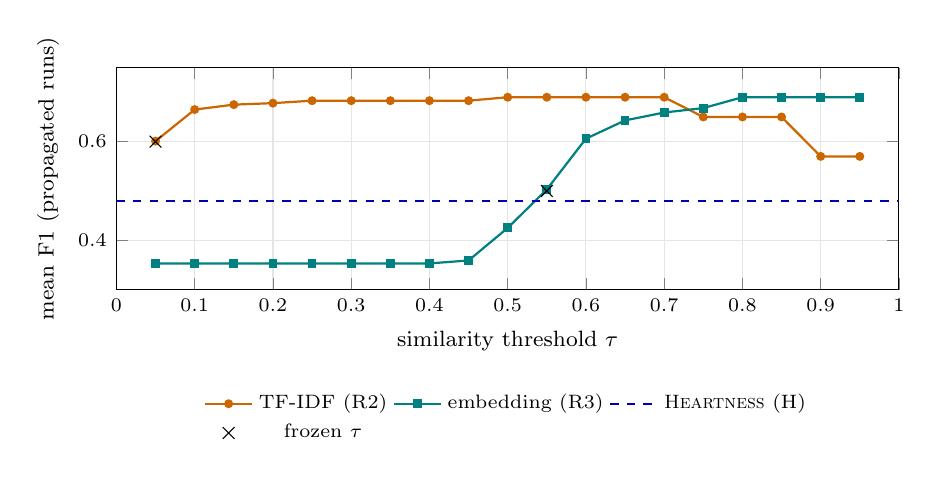
\begin{tikzpicture}
\begin{axis}[width=0.95\columnwidth, height=4.4cm, xlabel={similarity threshold $\tau$}, ylabel={mean F1 (propagated runs)}, xmin=0, xmax=1, ymin=0.3, ymax=0.75, legend style={font=\scriptsize, at={(0.5,-0.42)}, anchor=north, legend columns=3, draw=none}, tick label style={font=\scriptsize}, label style={font=\footnotesize}, grid=major, grid style={gray!20}]
\addplot[thick, mark=*, mark size=1.2pt, orange!80!black] coordinates {\LiveECurveTfidf};
\addplot[thick, mark=square*, mark size=1.2pt, teal] coordinates {\LiveECurveEmbed};
\addplot[thick, dashed, blue!70!black, domain=0:1] {\LiveEHFone};
\addplot[only marks, mark=x, mark size=3pt, black] coordinates {(\TauTfidf,\LiveERtwoFone) (\TauEmbed,\LiveERthreeFone)};
\legend{TF-IDF (R2), embedding (R3), \sys{} (H), frozen $\tau$}
\end{axis}
\end{tikzpicture}
\caption{F1 of the similarity baselines as a function of their threshold on the \LiveEPropagated{} propagated ExpeL-style runs, against \sys{}'s F1 (dashed). Crosses mark the thresholds frozen from the pilot. Because contaminated insights repeat the root closely, similarity reaches full recall over a wide range of thresholds.}\label{fig:thresholds}
\end{figure}

\emph{Results: detectors.} In this policy, content detectors were at least as good as closure. Fig.~\ref{fig:thresholds} shows that TF-IDF reached F1 between 0.66 and \LiveEBoundTfidfFone{} with full recall for every threshold from 0.10 to 0.70, and the embedding baseline did so from 0.70 upwards; at the frozen thresholds they reached \LiveERtwoFone{} and \LiveERthreeFone. Contaminated insights repeat the root closely, often verbatim, so the textual signal that similarity needs is present. The LLM judge (R4) was the most precise single detector (precision \LiveERfourPrecProp, F1 \LiveERfourFone) but missed the contaminated revisions of one propagated run (\texttt{llama3.1:8b}, F2, seed~1; recall \LiveERfourRec). \sys{} had lower F1 than R4 in \LiveETestFoneRfourLo{} and higher in \LiveETestFoneRfourHi{} of the \LiveEPropagated{} propagated runs, and lower than R2 in \LiveETestFoneRtwoLo{}; none of these differences is significant after Holm correction ($p\LiveETestFoneRfourP$ and $p\LiveETestFoneRtwoP$), which with ten informative runs mainly reflects low power.

\emph{Results: closure-bounded revalidation.} Revalidation recovers much of the detectors' precision while never looking outside the recorded closure. With the judge as screen (HS$_\mathrm{judge}$), \LiveEHSjudgeSuspProp{} revisions per propagated run stayed suspended instead of \LiveEHSuspProp{} (F1 \LiveEHSjudgeFone, the highest mean of all conditions at frozen settings), but it inherits the judge's one miss (recall \LiveEHSjudgeRec). With the embedding threshold (HS$_\mathrm{emb}$) it kept full recall at F1 \LiveEHSembedFone{} and was never worse than H. Compared with the stand-alone judge, HS$_\mathrm{judge}$ differs in \LiveEHSjudgeDiffersRfour{} of the \LiveEPropagated{} propagated runs; we therefore do not claim that it outperforms R4, only that the combination never affects anything outside the recorded lineage.

\emph{Results: ablations.} Removing EME edges or dependency edges changed the suspension set in \LiveEHnoEMEDiffers{} and \LiveEHnoDepsDiffers{} of \LiveERuns{} runs. In this policy this holds by construction and is not evidence about the edges: every insight in a run's context is also a source of the next extraction, so each EME edge coincides with a synthesis edge, and insights declare no use dependencies. The curation policy (below) separates the channels.

\emph{Results: behaviour.} Held-out pass@1 did not discriminate between remedies. Over all runs it was \LiveENonePass{} without remedy and \LiveEHPass{} after \sys{}, against \LiveEPassClean{} for the paired clean runs and \LiveEPassSeed{} for the hand-written harness without any learned state: on these held-out tasks, learned insights did not help, so suspending them could not show a cost. Inference is also not reproducible across processes: held-out prompts that were byte-identical in two different runs, and therefore generated independently, differed between pass and fail in \LiveENoiseFlips{} of \LiveENoisePairs{} pairs (\LiveENoiseRate\%). Almost all of these flips (\LiveENoiseFlipsNoLearned{}) occurred on prompts whose context held no learned insight, which recur across all runs of a cell and therefore form most pairs. Within one run, a repeated prompt is answered from the response cache, so the recorded runs replay exactly, but differences of a few items between remedies are within this noise. On the \LiveEPropagated{} propagated runs, mean pass@1 rose from \LiveENonePassProp{} to \LiveEHPassProp{} after \sys{}, but H was higher in \LiveEPassPropHigher{} runs and lower in \LiveEPassPropLower{} (Holm $p\LiveETestPassPropNoneP$). The fault-signature rate was the more sensitive signal: it fell from \LiveENoneSigProp{} to \LiveEHSigProp{} and was lower after \sys{} in \LiveETestSigPropNoneLo{} of the \LiveEPropagated{} runs and never higher ($p\LiveETestSigPropNoneP$, not significant). Removing contaminated insights thus removes the planted practice from the agent's code, but in our setting the effect on pass@1 is within inference noise.

\emph{Curation policy.} The curation policy builds the layered state of the running example, so it tests what the ExpeL-style policy could not: whether closure is narrower than a rollback, whether experience-mediated edges matter, and how detectors fare when faulty advice is folded into larger artifacts. Tables~\ref{tab:live-models-cur} and~\ref{tab:live-curate} report the \LiveCRuns{} faulty curation runs in the same format as before.

\begin{table}[!t]
\caption{Fault adoption and propagation per generator, curation policy (HumanEval+, \LiveSeeds{} seeds $\times$ 3 faults). Columns as in Table~\ref{tab:live-models}.}\label{tab:live-models-cur}
\centering\footnotesize
\setlength{\tabcolsep}{3pt}
\begin{tabular}{@{}lrrrrrrr@{}}
\toprule
Generator & Runs & Adopt. & Spread & Cont. & Live & H susp. & Clean\\
\midrule
\LiveCModelRows
\bottomrule
\end{tabular}
\end{table}

\begin{table*}[!t]
\caption{Containment in the live harness, curation policy. Columns as in Table~\ref{tab:live-expel}; Susp.~(prop.), precision, recall and F1 over the \LiveCPropagated{} propagated runs, all other columns over all \LiveCRuns{} faulty runs. H$_{\neg\mathrm{dep}}$ equals H by construction (every profile dependency is also a synthesis source); H$_\mathrm{local}$ suspends revisions in the store but cannot remove deployed copies, which agents keep loading. H$_\mathrm{EME\text{-}fail}$ counts EME exposure only for runs whose task failed.}\label{tab:live-curate}
\centering\footnotesize
\begin{tabular}{@{}lrrrrrrrrr@{}}
\toprule
Remedy & Susp. (all) & Susp. (prop.) & Precision & Recall & F1 & Residual & Collateral & Pass@1 & Signature\\
\midrule
\LiveCRows
\bottomrule
\end{tabular}
\end{table*}

\emph{Results (curation): adoption and spread.} Under curation a single corrupted message took hold far more often. The oracle found the planted practice in the root memory in \LiveCRootAdopted{} of \LiveCRuns{} runs (\LiveCAdoptedAmb{} counting ambiguous root labels) and in at least one further revision in \LiveCPropagated{} runs, with \LiveCContaminated{} contaminated derivatives in total. Every generator propagated the fault (Table~\ref{tab:live-models-cur}), and so did every fault type (F1 in \LiveCFonePropagated{} runs, F2 in \LiveCFtwoPropagated{}, F3 in \LiveCFthreePropagated{}). The contamination sat in the composed layers: \LiveCContSkill{} contaminated skills and \LiveCContProfile{} contaminated profiles, but only \LiveCContMemory{} memories. Once the curator had merged the faulty memory into a skill, the next profile composition typically restated it as one rule of the deployment's system prompt, which every later task then loaded (Section~\ref{sec:bg-example} quotes such a chain). The oracle labelled none of the \LiveCCleanRevisions{} revisions of the clean curation runs contaminated (\LiveCCleanLabelItems{} labels, \LiveCCleanAmbLabels{} ambiguous); the judges agreed on \LiveCJudgeRaw\% of \LiveCJudgeItems{} labels ($\kappa=\LiveCKappa$; positive agreement, the agreement on YES labels, \LiveCJudgePositive).

\emph{Results (curation): containment and detectors.} Doing nothing or deleting the root left \LiveCNoneResid{} contaminated derivatives loadable per run. \sys{} again suspended every contaminated derivative in all \LiveCPropagated{} propagated runs (recall \LiveCHRec{}, also \LiveCHRecAmb{} when ambiguous labels count as contaminated; residual \LiveCHResid). Unlike under the ExpeL-style policy, the detectors now missed contamination. The embedding baseline (recall \LiveCRthreeRec) missed it in \LiveCMissRunsRthree{} runs, mostly in profiles (\LiveCMissRthreeProfile{} of its misses), and the LLM judge (recall \LiveCRfourRec) in \LiveCMissRunsRfour{} runs, mostly in skills (\LiveCMissRfourSkill) and profiles (\LiveCMissRfourProfile); \sys{}'s recall was higher than R3's in \LiveCTestRecRthreeHi{} runs and R4's in \LiveCTestRecRfourHi{}, and never lower (Holm $p\LiveCTestRecRthreeP$ and $p\LiveCTestRecRfourP$). The mechanism is dilution: a skill or profile states the faulty practice in one of five or more rules, so the artifact as a whole is not similar to the root, and the generator, acting as judge, often did not flag such a rule. TF-IDF at the frozen threshold kept recall high (\LiveCRtwoRec, misses in \LiveCMissRunsRtwo{} runs). Its threshold is the lowest of the grid, so it suspends \LiveCRtwoSusp{} revisions per run, at precision \LiveCRtwoPrecProp. Fig.~\ref{fig:thresholds-cur} shows that no threshold gives both: the oracle-tuned optimum ($\tau_t=\LiveCBoundTfidfTau$, F1 \LiveCBoundTfidfFone) reaches recall \LiveCBoundTfidfRec, and the embedding baseline never exceeds F1 \LiveCBoundEmbedFone. Where the textual signal is diluted, a detector must trade recall for precision, and its thresholds cannot be validated without ground truth. On F1 and collateral the comparison reverses. TF-IDF and the LLM judge had higher F1 than \sys{} (the embedding detector was comparable: \LiveCRthreeFone{} against \LiveCHFone, \sys{} higher in \LiveCTestFoneRthreeHi{} runs and lower in \LiveCTestFoneRthreeLo, Holm $p\LiveCTestFoneRthreeP$), R2 in all \LiveCPropagated{} propagated runs (Holm $p\LiveCTestFoneRtwoP$). R4 had higher F1 than \sys{} in \LiveCTestFoneRfourLo{} of them and lower in \LiveCTestFoneRfourHi{} ($p\LiveCTestFoneRfourP$), and \sys{} suspended more clean revisions than R2 in \LiveCTestCollRtwoHi{} and than R4 in \LiveCTestCollRfourHi{} of \LiveCRuns{} runs ($p\LiveCTestCollRtwoP$ and $p\LiveCTestCollRfourP$), and more than R3 in \LiveCTestCollRthreeHi{} (fewer in \LiveCTestCollRthreeLo; $p\LiveCTestCollRthreeP$). All contamination metrics here have an effective sample of \LiveCPropagated{} runs.

\begin{figure}[!t]
\centering
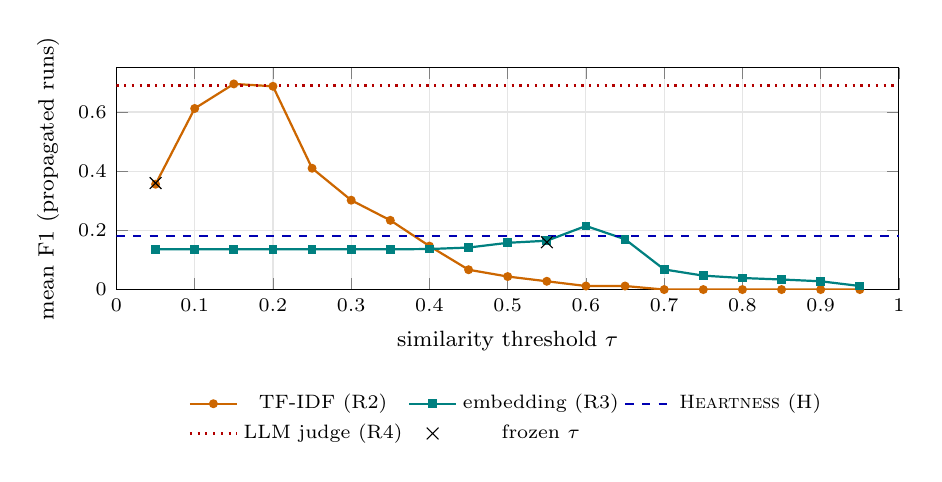
\begin{tikzpicture}
\begin{axis}[width=0.95\columnwidth, height=4.4cm, xlabel={similarity threshold $\tau$}, ylabel={mean F1 (propagated runs)}, xmin=0, xmax=1, ymin=0, ymax=0.75, legend style={font=\scriptsize, at={(0.5,-0.42)}, anchor=north, legend columns=3, draw=none}, tick label style={font=\scriptsize}, label style={font=\footnotesize}, grid=major, grid style={gray!20}]
\addplot[thick, mark=*, mark size=1.2pt, orange!80!black] coordinates {\LiveCCurveTfidf};
\addplot[thick, mark=square*, mark size=1.2pt, teal] coordinates {\LiveCCurveEmbed};
\addplot[thick, dashed, blue!70!black, domain=0:1] {\LiveCHFone};
\addplot[thick, dotted, red!70!black, domain=0:1] {\LiveCRfourFone};
\addplot[only marks, mark=x, mark size=3pt, black] coordinates {(\TauTfidf,\LiveCRtwoFone) (\TauEmbed,\LiveCRthreeFone)};
\legend{TF-IDF (R2), embedding (R3), \sys{} (H), LLM judge (R4), frozen $\tau$}
\end{axis}
\end{tikzpicture}
\caption{F1 of the similarity baselines as a function of their threshold on the \LiveCPropagated{} propagated curation runs, against \sys{} (dashed) and the LLM judge (dotted). Unlike under the ExpeL-style policy (Fig.~\ref{fig:thresholds}), F1 peaks sharply at a low threshold, where TF-IDF recall is \LiveCBoundTfidfRec{}; among the plotted conditions, only \sys{} and R2 at the frozen threshold have recall near 1.}\label{fig:thresholds-cur}
\end{figure}

\emph{Results (curation): closure versus the time cut.} Here the closure was strictly narrower than a rollback. \sys{} suspended \LiveCHSusp{} revisions per run against \LiveCTcutSusp{} for the time cut T and \LiveCAresetSusp{} for resetting all learned state; its suspension set was contained in T's in all \LiveCCutSubset{} runs, as Proposition~\ref{prop:cut} requires, and strictly smaller in \LiveCCutStrict{}, with equal recall. The difference is small, and its location explains why. All \LiveCCutGap{} revisions that T suspends and \sys{} spares are memories created between the fault and the first profile composition (after task~12) by tasks that never loaded the faulty memory or anything derived from it. From the composition on, the deployment's profile is in the closure (in \LiveCProfilesInClosure{} of \LiveCRuns{} runs), every task loads its profile, and so every later experience, and every memory written from it, is exposed. It is the EME rule applied to a broadcast context that pulls the closure up to the time cut: the precision of closure-based withdrawal depends jointly on how selectively the harness assembles contexts and on which runs count as exposure. The size of the gap is therefore a function of the fault position relative to the first composition: closure was strictly smaller than T in \LiveCCutStrictTaskTwo{} of \LiveCRunsTaskTwo{} runs with the fault at task~2, \LiveCCutStrictTaskEight{} of \LiveCRunsTaskEight{} at task~8 and \LiveCCutStrictTaskNine{} of \LiveCRunsTaskNine{} at task~9; faults after the first composition (task~12) were not sampled; there the next composition is at task~24, so later tasks would be exposed only through memory retrieval and the gap could be larger. In absolute terms \sys{}'s precision remained low (\LiveCHPrecProp, F1 \LiveCHFone), below every detector's, by a large margin for R2 and R4 and narrowly for R3. Withdrawing only the root that the oracle labels faulty (H$_\mathrm{faulty}$) would have missed contamination in \LiveCTestRecHfaultyHi{} runs whose derivatives were labelled contaminated but whose root was not; in all \LiveCFaultyMissAmbiguous{} the judges disagreed on the root. An operator who withdraws only revisions that look wrong inherits such misses, which is why H withdraws every revision motivated by the suspicious experience. Restricting attention to the \LiveCRootAdopted{} runs whose root adopted the fault does not change the picture: \sys{} suspended \LiveCAdoptHSusp{} revisions per run there, against \LiveCAdoptTcutSusp{} for T and \LiveCAdoptRfourSusp{} for R4.

\emph{Results: selectivity beyond the sampled fault positions.} Our planted faults fell at tasks 2, 8 and 9, before the first composition. Because closure and the time cut are computed from recorded structure alone, we can compare them for revisions created at any other position without the oracle, assuming that a fault there would leave the recorded exposure structure unchanged: we took every revision active at the end of each of the \LiveTotalRuns{} runs (faulty and clean) as a hypothetical root and compared its closure with the revisions written at later tasks (Table~\ref{tab:selectivity}; revisions written in the same step as the root are excluded, since a step-level rollback could also spare them). This measures only how much closure spares, not whether what it spares is clean. Under the ExpeL-style policy closure equalled the time cut for every root: every later extraction step sees the whole list. Under curation, roots created after the first composition had closures covering on average \LiveCSelThreeRatio{} (tasks 13--18) and \LiveCSelFourRatio{} (tasks 19--24) of the later revisions (fewer than all for \LiveCSelThreeStrict\% and \LiveCSelFourStrict\% of them; in absolute terms, \LiveCSelThreeSpared{} of \LiveCSelThreeLater{} and \LiveCSelFourSpared{} of \LiveCSelFourLater{} later revisions spared on average), against \LiveCSelTwoRatio{} for roots at tasks 7--12, because a memory written after task 12 reaches later contexts only through retrieval until the next composition. The sparing is a window effect: the profiles composed at task 24 were in the closure of every such root (\LiveCSelThreeReachFinal{} and \LiveCSelFourReachFinal{} roots), so after the next broadcast composition the closure would again reach the time cut, which is also why roots at tasks 19--24, whose later revisions include the task-24 profiles and skill, show a higher ratio than those at tasks 13--18. The low ratios therefore partly reflect the 24-task horizon. Counting EME only for failed runs lowered the ratios further (\LiveCSelTwoRatioFail{} for tasks 7--12). Closure is thus nearly a time cut for early revisions and exactly one for policies that show every step everything, and markedly more selective for revisions created after the first composition under retrieval, until the next composition.

\begin{table}[!t]
\caption{Structural selectivity: mean share of the revisions written at later tasks that fall in $\Cl(r)$, over every final active revision $r$ taken as a hypothetical root, by the task that created $r$, with the share of roots whose closure misses at least one later revision (Smaller). EME-fail: EME counted only for failed runs. Oracle-free; all \LiveTotalRuns{} runs; roots are the revisions still active at the end of a run (insights edited or removed earlier are not roots), and roots without later revisions are omitted. The ExpeL-style 1--6 row rests on a single root.}\label{tab:selectivity}
\centering\footnotesize
\setlength{\tabcolsep}{2pt}
\begin{tabular}{@{}lrrrrrrrr@{}}
\toprule
 & \multicolumn{4}{c}{ExpeL-style} & \multicolumn{4}{c}{Curation} \\
\cmidrule(lr){2-5}\cmidrule(l){6-9}
Root task & Roots & Ratio & EME-fail & Smaller & Roots & Ratio & EME-fail & Smaller \\
\midrule
1--6 & \LiveESelOneRoots & \LiveESelOneRatio & \LiveESelOneRatioFail & \LiveESelOneStrict\% & \LiveCSelOneRoots & \LiveCSelOneRatio & \LiveCSelOneRatioFail & \LiveCSelOneStrict\% \\
7--12 & \LiveESelTwoRoots & \LiveESelTwoRatio & \LiveESelTwoRatioFail & \LiveESelTwoStrict\% & \LiveCSelTwoRoots & \LiveCSelTwoRatio & \LiveCSelTwoRatioFail & \LiveCSelTwoStrict\% \\
13--18 & \LiveESelThreeRoots & \LiveESelThreeRatio & \LiveESelThreeRatioFail & \LiveESelThreeStrict\% & \LiveCSelThreeRoots & \LiveCSelThreeRatio & \LiveCSelThreeRatioFail & \LiveCSelThreeStrict\% \\
19--24 & \LiveESelFourRoots & \LiveESelFourRatio & \LiveESelFourRatioFail & \LiveESelFourStrict\% & \LiveCSelFourRoots & \LiveCSelFourRatio & \LiveCSelFourRatioFail & \LiveCSelFourStrict\% \\
\bottomrule
\end{tabular}
\end{table}

\emph{Results (curation): which edges matter.} Without EME edges, the closure changed in \LiveCHnoEMEDiffers{} of \LiveCRuns{} runs: it suspended \LiveCHnoEMESusp{} instead of \LiveCHSusp{} revisions per run (F1 \LiveCHnoEMEFone{} instead of \LiveCHFone) but left contamination loadable in \LiveCEMEOnlyRuns{} run. That run is the behavioural inheritance of the running example: in \texttt{llama3.1:8b}, F3, seed~3, the corrupted feedback produced memory $m_8$ (\emph{``\ldots use integer division (//) instead of true division (/)\ldots''}); the next task retrieved $m_8$ into its context, the agent's solution used floor division, and the reflection, shown only two unrelated memories as sources, wrote $m_9$: \emph{``\ldots consider using the // operator for integer division instead of the / operator\ldots''}. Only the exposure of that run to $m_8$ connects $m_9$ to the fault. EME edges therefore bought one contaminated revision in \LiveCPropagated{} propagated runs at the price of more collateral in \LiveCTestCollHnoEMEHi{} runs, on average \LiveCHSusp{} instead of \LiveCHnoEMESusp{} suspended revisions per run. EME is a policy of the controller, not a fixed rule: counting exposure only for runs whose task failed (H$_\mathrm{EME\text{-}fail}$, a post-hoc variant computed from the recorded state) kept recall \LiveCHEMEfailRec{} including the run above, whose task had failed, and suspended \LiveCHEMEfailSusp{} revisions per run (F1 \LiveCHEMEfailFone); whether that price is worth paying depends on how costly a residual faulty lesson is relative to a temporarily suspended clean one, which is a deployment decision, not one our data can settle. Dependency edges changed nothing (\LiveCHnoDepsDiffers{} runs differ) because every profile's dependencies on skills are also its synthesis sources; dependency-only consumers are covered by the synthetic motifs of E-Q. Withdrawal without deployment propagation (H$_\mathrm{local}$) left contamination in use in every propagated run (recall \LiveCHlocalRec).

\emph{Results (curation): revalidation.} Closure-bounded revalidation is limited by its screen, and helped by the dependency rule of Algorithm~\ref{alg:reval}. With the judge as screen, HS$_\mathrm{judge}$ kept \LiveCHSjudgeSuspProp{} revisions per propagated run suspended (F1 \LiveCHSjudgeFone) but, like the judge alone, restored contaminated revisions in \LiveCTestResidHSjudgeLo{} runs (recall \LiveCHSjudgeRec); under curation it differs from the judge alone in \LiveCHSjudgeDiffersRfour{} of \LiveCPropagated{} propagated runs but has the same recall and slightly lower F1 (\LiveCRfourFone{} for R4) because \LiveCHSjudgeRejected{} cleared profiles, none of them contaminated, were rejected while a skill they depend on stayed suspended. With the embedding screen the rule mattered: the screen cleared \LiveCHSembedRejectedCont{} contaminated revisions whose dependencies it did not clear, and admission rejected them (\LiveCHSembedRejected{} rejections in \LiveCHSembedRejectedRuns{} runs), so HS$_\mathrm{emb}$ reached recall \LiveCHSembedRec{} against \LiveCRthreeRec{} for the same screen applied to the whole state (R3). Revalidation never touches anything outside the closure, but under curation it cannot recover the detectors' precision without giving up part of the closure's recall; a screen with higher recall than the generator-as-judge would be needed.

\emph{Results (curation): behaviour.} Held-out pass@1 was again uninformative: \LiveCNonePass{} without remedy, \LiveCHPass{} after \sys{}, \LiveCPassClean{} for the clean runs and \LiveCPassSeed{} for the hand-written harness. On the \LiveCPropagated{} propagated runs it rose from \LiveCNonePassProp{} to \LiveCHPassProp{} after \sys{} (higher in \LiveCPassPropHigher{} runs, lower in \LiveCPassPropLower{}, Holm $p\LiveCTestPassPropNoneP$), and the fault-signature rate fell from \LiveCNoneSigProp{} to \LiveCHSigProp{} (lower in \LiveCTestSigPropNoneLo{} runs, higher in \LiveCTestSigPropNoneHi{}, Holm $p\LiveCTestSigPropNoneP$). Under both policies the means move in the expected direction, and neither difference is significant. The propagated-run gain in pass@1 corresponds to less than one of \LiveEvalTasks{} held-out items per run. Byte-identical prompts generated independently in two runs differed in \LiveCNoiseFlips{} of \LiveCNoisePairs{} pairs (\LiveCNoiseRate\%) under curation (\LiveENoiseRate\% under the ExpeL-style policy).


\subsubsection{Experiment E-Q: lineage queries with exact ground truth}
\emph{Objective.} Separate the accuracy of the queries on which containment rests (origins of a revision, its descendants, and the affected set of a withdrawal) from the accuracy of the content oracle. \emph{Procedure.} On \TraceCases{} synthetic scenarios (nine structural motifs $\times$ three sizes $\times$ 30 seeds) each method answered all three queries for every revision, scored by F1 against construction-time truth. A separate configuration rewrote 0\%, 50\% or 100\% of each derived revision's text while keeping its lineage.

\emph{Results.} Recorded exposure answered all queries exactly (impact F1 \SynOursImpact), within-file history recovered almost none of the cross-file lineage (impact \SynHistoryImpact, descendants \SynHistoryDescendants), and lexical recovery was in between (impact \SynLexicalImpact, origins \SynLexicalOrigins). Paraphrasing lowered lexical impact F1 from \ParaLexicalZero{} (no rewriting) to \ParaLexicalHalf{} and \ParaLexicalFull{} (half and full rewriting) and did not affect recorded exposure. As intended, the capture-only baseline answers the queries exactly as \sys{} does (impact \SynCaptureOnlyImpact): with complete edges the query is the same reachability computation. What capture alone lacks is shown elsewhere: H$_\mathrm{local}$ in E-L (no deployment-wide suspension), and RQ2 (no admission or rollback guards). A direct-edge linter that flags revisions with a withdrawn parent, without transitive propagation, reached F1 \LinterFOne{} on \LinterCases{} post-withdrawal states with \LinterBenign{} false alarms on clean controls: transitive closure, not detection of direct parents, is what finds the affected set.

\subsubsection{Experiment E-K: sensitivity to capture completeness}
\emph{Objective.} Quantify how much containment depends on the completeness of capture (assumption A2). \emph{Procedure.} We hid a random 0--100\% of the derivation edges from each method before querying, 30 seeds per level.

\begin{figure}[!t]
\centering
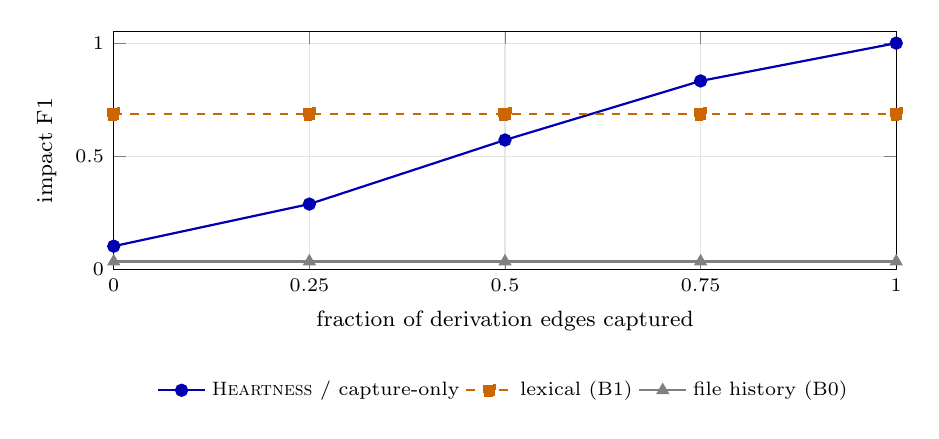
\begin{tikzpicture}
\begin{axis}[width=0.95\columnwidth, height=4.6cm, xlabel={fraction of derivation edges captured}, ylabel={impact F1}, xmin=0, xmax=1, ymin=0, ymax=1.05, xtick={0,0.25,0.5,0.75,1}, legend style={font=\scriptsize, at={(0.5,-0.42)}, anchor=north, legend columns=3, draw=none}, tick label style={font=\scriptsize}, label style={font=\footnotesize}, grid=major, grid style={gray!20}]
\addplot[thick, mark=*, blue!70!black] coordinates {\CaptureCoordsOurs};
\addplot[thick, mark=square*, orange!80!black, dashed] coordinates {\CaptureCoordsLexical};
\addplot[thick, mark=triangle*, gray] coordinates {\CaptureCoordsHistory};
\legend{\sys{} / capture-only, lexical (B1), file history (B0)}
\end{axis}
\end{tikzpicture}
\caption{Impact F1 as capture completeness varies (synthetic benchmark, 30 seeds per point). Recorded exposure degrades in proportion to missing edges; somewhere between 50\% and 75\% capture, lexical recovery becomes more accurate.}\label{fig:capture}
\end{figure}

\emph{Results.} Fig.~\ref{fig:capture} shows that recorded exposure is only as good as its capture: impact F1 fell from \CaptureOursFull{} with complete capture to \CaptureOursThreeQuarters, \CaptureOursHalf{} and \CaptureOursQuarter{} with 75\%, 50\% and 25\% of the edges, and to \CaptureOursZero{} with none, whereas lexical recovery, which does not use edges, stayed at \CaptureLexicalFull. Somewhere between half and three quarters of the edges, a lexical detector becomes the better tool. This is the quantitative reason for host-side capture (Section~\ref{sec:capture}): the controller, not the policy, must record exposure, and it must do so for every input it supplies.

\noindent\fbox{\parbox{0.96\columnwidth}{\textbf{Answer to RQ1.} Closure-based withdrawal had recall 1.00 in all \LivePropagatedAll{} propagated runs, as did rollback, reset and the EME-fail variant. What it suspends is bounded by the time cut: the same set under the ExpeL-style policy, slightly less under curation. Every detector was more precise, and under curation TF-IDF and the LLM judge had significantly higher F1, but detectors missed contamination folded into skills and profiles (R3: \LiveCMissRunsComposedRthree, R4: \LiveCMissRunsComposedRfour, R2: \LiveCMissRunsComposedRtwo{} of \LiveCPropagated{} runs). Structurally, closure is markedly more selective than a time cut only for curation revisions created after the first composition, and only until the next composition. EME edges were necessary once, at a large collateral cost. Effects on held-out behaviour were not significant.}}


\subsection{RQ2: Assurance of the Lifecycle Guards}\label{sec:rq2}
\emph{RQ2: Do the lifecycle guards prevent property violations that their removal would allow, and does bounded model checking find such violations with witnesses that hold on the implementation?}

\subsubsection{Experiment E-G: targeted guard challenges}
\emph{Objective.} Establish, guard by guard, that each guard or audit predicate is what prevents or exposes a specific violation, rather than assuming it. \emph{Procedure.} For each property P1--P10 we construct one challenge on the running example that targets it: an inadmissible event for guard-enforced properties (P1--P4, P6, P8, P9), and out-of-API corruption of the stored state for the audit-only properties (P5, P7, P10). Each challenge runs twice: on the full engine and on an engine with the targeted guard (or audit predicate) removed.

\emph{Results.} With all guards present, every guard-enforced challenge was either rejected (P1, P3, P4, P6, P9) or contained without any violation (P2, P8: suspension removes the affected revisions); the out-of-API corruptions were flagged by the audit (P5, P7, P10). Removing the targeted guard or predicate changed the outcome of \GuardRemovedAlarms{} of the \GuardChallenges{} challenges to the targeted failure: the event was admitted and the audit reported the targeted violation, or the corruption went unreported. Removing the withdrawal guard (the P2 suspension) also produced a P8 violation, because the same suspension protects deployments. The result is close to definitional, and the mutation tests (Section~\ref{sec:impl}) already show that the test suite detects removed guards; what E-G adds is a property-by-property map from each guard to the concrete violation it prevents on the running example, which the bounded checks of E-M then generalize over all short operation sequences.

\subsubsection{Experiment E-M: bounded model checking and witness replay}
\emph{Objective.} Check whether the guard semantics admit any violating operation sequence within a bound, and whether violations found on the model also occur on the implementation. \emph{Procedure.} For three identities, the three topologies and a depth bound of 10 operations, we ran the reference projection and five guard mutants (P2, P3, P4, P8, P9 removed) through both the Python BFS and SPIN (18 configurations), replayed every BFS witness on the projection and on the engine with the same guard disabled, and re-ran BFS at depth $\ell-1$ to check minimality. A separate experiment (E-C) compared engine and projection on every successor of all reference states reachable within depth~6 for two identities, under an explicit state mapping.

\begin{table}[!t]
\caption{Bounded model checking (3 identities, depth 10). States: BFS states explored. SPIN s: SPIN verification time. Verdict: BFS verdict and shortest witness length; Agree: SPIN verdict equals BFS verdict.}\label{tab:checking}
\centering\footnotesize
\begin{tabular}{@{}llrrll@{}}
\toprule
Guards & Topology & States & SPIN s & Verdict & Agree\\
\midrule
\CheckerRows
\bottomrule
\end{tabular}
\end{table}

\emph{Results.} Table~\ref{tab:checking} lists all 18 configurations. BFS and SPIN agreed on \CheckerAgreements/\CheckerComparisons{} verdicts. The reference guards were safe within the bound in all topologies (up to \MaxReferenceStates{} states). \CheckerViolating{} mutant configurations violated a property, with shortest witnesses of \WitnessMin--\WitnessMax{} operations; all \ReplaySuccesses{} witnesses replayed on the engine with the same guard removed and produced the targeted audit violation, and all \MinimalWitnesses{} were minimal (no violation at depth $\ell-1$). The \CheckerSafeMutants{} remaining mutant configurations (P2 and P3 removed, independent topology) were safe, as expected: without edges there is nothing for those guards to protect. They act as negative controls showing that the checker does not report violations indiscriminately. In E-C, \MappedTransitions{} attempted transitions (\MappedEnabled{} enabled) were compared and \MappedMismatches{} mismatches were found.

These checks also paid off during development, which is a qualitative result in its own right. In an earlier campaign (retained in the replication package), replaying model-checking witnesses on the engine failed for four witnesses. The cause was a missing guard in the abstract specification (proposals could cite a source that had not been installed), shared by both encodings, and it was invisible to verdict agreement alone. A second discrepancy, found by mapped-state comparison, concerned whether \textsc{Deploy} replaces or extends deployment membership. Both were fixed in the specification and the implementation, and all reported campaigns use the corrected versions.

\subsubsection{Experiment E-S: exhaustive versus sampled exploration}
\emph{Objective.} Assess whether exhaustive bounded exploration is needed, or whether cheaper randomized or property-based testing finds the same guard faults. \emph{Procedure.} For two identities and depth~9, 30 trials per mutant ran uniform random sequences and Hypothesis-generated sequences under the same wall-clock budget as BFS.

\begin{table}[!t]
\caption{Guard faults detected out of 30 trials under equal time budgets (2 identities, depth 9).}\label{tab:search}
\centering\footnotesize
\begin{tabular}{@{}lrrr@{}}
\toprule
Guard removed & Random & Hypothesis & BFS\\
\midrule
\SearchRows
\bottomrule
\end{tabular}
\end{table}

\emph{Results.} Table~\ref{tab:search} shows that BFS detected every seeded fault in every trial and raised no false alarm on the reference guards. Random sequences found the faults that need few, unconstrained steps (P4, P9, and P8 in most trials) but rarely or never found those that need a specific ordering of acceptance, withdrawal and re-acceptance (P2, P3); Hypothesis did worse on most faults under the same budget. The faults that sampling misses are precisely those concerning withdrawn lineage.

\emph{Discussion.} The guards are individually necessary for their properties, exhaustive bounded exploration is necessary to find ordering-dependent faults reliably, and witness replay plus mapped-state comparison catch model--implementation mismatches that verdict agreement does not. The evidence remains bounded: three identities, depth 10, a projection without text, effects or EME, and with contracts reduced to the presence of dependencies.

\noindent\fbox{\parbox{0.96\columnwidth}{\textbf{Answer to RQ2.} Each guard prevents its targeted violation (\GuardRemovedAlarms/\GuardChallenges{} targeted challenges change outcome when it is removed). Within the checked bounds the reference lifecycle is safe; BFS and SPIN agree on all \CheckerComparisons{} configurations; all \ReplaySuccesses{} witnesses are minimal and reproduce on the implementation; and, on seeded guard faults at small scope, exhaustive exploration finds ordering-dependent withdrawal faults that equal-budget random and property-based testing miss.}}

\subsection{RQ3: Cost and Limits}\label{sec:rq3}
\emph{RQ3: What do capture, admission, withdrawal and checking cost, and what can runtime conformance monitoring detect or not detect?}

\subsubsection{Experiment E-O: overhead in the live harness}
\emph{Objective.} Measure the controller's share of the cost of real self-evolution. \emph{Procedure.} In every live run we timed all controller calls (capture, admission, snapshots, \textsc{Load}) separately from LLM generation and test execution, and timed each remedy.

\emph{Results.} The controller is a negligible part of live self-evolution. In the ExpeL-style runs, one run took \LiveEEvolveMinutes{} minutes of evolution on average (\LiveELLMCalls{} LLM calls, about \LiveETokensIn{}k input and \LiveETokensOut{}k output tokens), of which all controller operations together (capture, admission, snapshots, \textsc{Load} and deployment updates, about \LiveEHistoryEvents{} history events) took \LiveEEngineSeconds{}\,s, or \LiveEEnginePercent\% of the evolution time. Computing a withdrawal plan with \sys{} took \LiveEHMs\,ms per run, against \LiveERtwoMs\,ms for TF-IDF, \LiveERthreeMs\,ms for the embedding baseline (dominated by embedding calls) and \LiveERfourMs\,ms for the LLM judge, which must read every live revision. Under curation, contexts and state are larger (\LiveCEvolveMinutes{} minutes, \LiveCLLMCalls{} LLM calls and about \LiveCHistoryEvents{} history events per run); the controller took \LiveCEngineSeconds{}\,s, or \LiveCEnginePercent\% of evolution time, and a withdrawal plan \LiveCHMs\,ms against \LiveCRfourMs\,ms for the LLM judge. Revalidation adds judge or embedding calls only for members of the closure.


\subsubsection{Experiment E-T: scaling of controller operations}
\emph{Objective.} Separate the cost of graph queries from that of full transactional admission and replay as state grows. \emph{Procedure.} Closure queries on synthetic graphs of up to 2{,}048 revisions (30 seeds); complete guarded workloads of 4--32 artifacts (30 seeds each) measuring capture, admission, withdrawal and monitor replay under Python allocation tracing; and the BFS state space of the projection for 2--6 identities.

\begin{table}[!t]
\caption{State-space growth of exhaustive exploration over the full engine (depth 10, at most 20{,}000 states). $n$: revision identities; States: reachable engine states explored; Time: wall-clock seconds; Complete: whether exploration finished below the cap.}\label{tab:scale}
\centering\footnotesize
\begin{tabular}{@{}rlrrl@{}}
\toprule
$n$ & Topology & States & Time (s) & Complete\\
\midrule
\ScaleRows
\bottomrule
\end{tabular}
\end{table}

\emph{Results.} A closure query over 2{,}048 revisions took \GraphMilliseconds{}\,ms on average (\GraphKilobytes{}\,KB peak). Full guarded workloads are far more expensive: with 32 artifacts and about \HistoryEventsThirtyTwo{} history events, admission of the whole workload took \AdmissionMsThirtyTwo\,ms, withdrawal \WithdrawalMsThirtyTwo\,ms, and replaying the history in the monitor \MonitorMsThirtyTwo\,ms, versus \AdmissionMsFour\,ms, \WithdrawalMsFour\,ms and \MonitorMsFour\,ms for 4 artifacts. Admission and replay grow super-linearly because the prototype deep-copies state for atomicity and recomputes closures on every acceptance. Table~\ref{tab:scale} shows how quickly exhaustive exploration of the full engine grows with the number of identities: with independent revisions it hits the 20{,}000-state cap from three identities on, while a chain stays below 6{,}100 states up to six identities because its dependencies forbid most interleavings. This is why the model checking of RQ2 uses the finite projection rather than the engine.

\subsubsection{Experiment E-R: what conformance monitoring detects}
\emph{Objective.} Determine which deviations between logged events and real state the monitor detects. \emph{Procedure.} On the running example, 30 seeded positions each for five scenarios: benign logs, observed-state drift (a revision edited outside the API), invalid events, omitted events, and hidden external actions that are never logged.

\emph{Results.} The monitor reported no deviation on \MonBenign/\MonN{} benign logs and detected \MonDrift/\MonN{} drifts, \MonInvalid/\MonN{} invalid events and \MonOmitted/\MonN{} omitted events. It detected \MonHidden/\MonN{} hidden external actions: an action that is never logged leaves no trace for a log-based monitor. Across \RemediationRuns{} withdrawal-and-rollback scenarios, \UnsafeRollbackRejected{} rollbacks into withdrawn lineage were rejected and external effects were retained in all \EffectsRetained{}. Replaying the \PublicRevisions{} Voyager skill-library revisions (\PublicEvents{} events) through the controller produced no conformance finding, showing that the metamodel accepts a real third-party evolution history (this replay does not reconstruct how the skills were synthesized).

\noindent\fbox{\parbox{0.96\columnwidth}{\textbf{Answer to RQ3.} In live self-evolution the controller costs \LiveEEnginePercent\% (ExpeL-style) and \LiveCEnginePercent\% (curation) of evolution time, and a withdrawal plan takes milliseconds where an LLM-judge screening takes tens of seconds. Closure queries are cheap even for thousands of revisions, but full transactional admission and replay in our prototype grow super-linearly and reach 1--3\,s for 32-artifact workloads; finite checking scales only to a handful of identities. The monitor detects drift, invalid events and nearly all omissions, and by construction cannot detect actions that are never logged.}}

\subsection{Threats to Validity}\label{sec:threats}
\emph{Construct validity.} Our ground truth for contamination is a content oracle of two LLM judges, not human annotation. We mitigate this by using judges from families different from every generator, schema-constrained answers, unanimity, reporting ambiguous labels and their effect, measuring agreement ($\kappa$), checking the judges' false-positive rate on clean runs, and complementing content labels with behavioural measures (HumanEval+ tests and static fault signatures). A judge can still miss a paraphrase or flag an artifact that merely mentions the practice. Exposure, which \sys{} records, is not influence; we therefore never evaluate \sys{} against its own records but against content and behaviour. Pass@1 on held-out tasks measures one aspect of harness quality and is sensitive to which state remains loadable; a remedy that removes useful state is penalized only insofar as that state helped on those tasks. In the synthetic benchmark, ground truth is exact by construction but its structures are generated, and with complete capture \sys{} and capture-only provenance answer queries identically by design.

\emph{Internal validity.} The faults are planted by corrupting one feedback message; real faulty lessons can arise more gradually or from several experiences. The fault position took only three values (tasks \LiveEFaultPositions) for our seeds; early faults favour propagation and inflate closure sizes relative to late faults. Revalidation and the post-hoc conditions (T, A, H$_\mathrm{faulty}$) were designed after the local pilot, and H$_\mathrm{EME\text{-}fail}$ after the first analysis of the reported campaign, when the single run that only EME edges trace was known to have failed; its recall therefore rests on that run. The structural selectivity analysis was added late, in response to internal review of an earlier version of this paper, and its definition was revised once: a first version that counted revisions written in the same step as the root made the ExpeL-style policy look selective for late roots, which it is not. Revalidation was re-run once on the curation records with the dependency rule of Algorithm~\ref{alg:reval}, after a review found that the first evaluation had not applied it; the superseded results are kept in the package; revalidation was evaluated on the recorded state in a separate process rather than through the controller's admission operators. Thresholds of the similarity baselines were tuned on a local pilot with a different generator (\texttt{qwen2.5:7b}) and the curation policy and transferred unchanged to all generators and both policies; tuning per model and policy could improve them, which we bound with an oracle-tuned upper bound. The R4 judge is the generator itself, as a harness would use it; a stronger external judge could detect more, but would then be close to the oracle. LLM decoding used temperature~0 and fixed seeds, but batched GPU inference is not reproducible across processes: byte-identical prompts generated independently in two runs flipped pass/fail in \LiveENoiseRate\% (ExpeL-style) and \LiveCNoiseRate\% (curation) of pairs. On \LiveCCPUCells{} of the \LiveCOracleCells{} oracle jobs of the curation campaign the inference server fell back to CPU because GPU discovery timed out; those judges ran at temperature~0 and their labels were kept. Generation jobs whose server fell back to CPU failed, found their cells already complete, or (after we added a device check to the job script) restarted the server until it ran on GPU, so every reported evolution run and revalidation was generated on GPU (\texttt{inference\_devices.tsv} in the package lists the device of every job). Every response is cached, so the reported runs replay exactly, while a fresh run reproduces the protocol rather than the exact texts. The harness, the remedies and the oracle prompts were written by us; we report all prompts in the replication package.

\emph{Platform validity.} The live study ran on one cluster and one GPU type; we did not measure how much results vary across hardware, because the smoke runs on other sites were too short (8 tasks, one seed) to say. All compared conditions share the platform, which protects the comparisons but not the absolute numbers.

\emph{External validity.} The live harness is small (24 evolution tasks, two deployments) compared with production agents, and the tasks are function-level Python problems; the two harness policies (curation into skills and profiles, and ExpeL-style insight lists) are two of many update mechanisms~\cite{wei2026harness}. We used five open-weight 7--16B generators; larger proprietary models may follow or filter faulty lessons differently. Capture completeness holds only for inputs the host mediates (assumption A2); production harnesses with tool results, web content or shared memories across users would need corresponding instrumentation. The synthetic benchmark and the bounded model checking cover small graphs and few identities.

\emph{Conclusion validity.} Each faulty run is a paired observation across remedies; we use non-parametric paired tests, effect sizes and Holm correction, and ship bootstrap confidence intervals with the per-run values. Runs in which the generator did not adopt the planted fault, or in which it did not propagate beyond the root, carry no information about recall; we report how many there were and compute precision, recall and F1 only on the others, which reduces the effective sample size for those metrics to \LiveEPropagated{} of \LiveERuns{} ExpeL-style and \LiveCPropagated{} of \LiveCRuns{} curation runs. We named no single primary metric; recall and residual contamination are the metrics the approach is designed for, and we report all others with equal prominence, including those that favour the detectors. Differences that are consistent in direction but not significant after correction are reported as such.

\subsection{Lessons Learned and Limitations}\label{sec:lessons}
\emph{Report adoption, not only containment.} A corrupted feedback message became a contaminated revision in only part of the faulty runs, and how often depended strongly on the generator, the fault and the policy: propagation occurred in \LiveEPropagated{} of \LiveERuns{} ExpeL-style runs but \LiveCPropagated{} of \LiveCRuns{} curation runs (Tables~\ref{tab:live-models} and~\ref{tab:live-models-cur}). A containment study that plants faults and reports only averages over all runs would mostly measure runs with nothing to contain. We therefore report adoption and propagation counts, compute recall only where there was something to recall, and recommend the same for future studies of faulty or poisoned self-evolution.

\emph{The policy decides what closure costs.} Closure suspends what was \emph{exposed}, and how much is exposed is a design decision of the self-evolving policy. By Proposition~\ref{prop:cut}, withdrawal never suspends more than a rollback to before the fault, and in our ExpeL-style runs, where every extraction step sees the whole insight list, it suspended exactly as much. Under curation it was smaller only until the first composed profile was deployed; from then on every task loaded it, and EME edges made every later lesson exposed. Conversely, for roots created after that composition, which reach later contexts only through retrieval, closures covered on average \LiveCSelThreeRatio--\LiveCSelFourRatio{} of the later state (Table~\ref{tab:selectivity}), but only until the next broadcast composition. Harness designers who want withdrawal to be cheaper than a rollback must give each generation step and each run only the inputs it needs, because the host records exactly what it supplies, and can restrict which runs count as exposure: counting only failed runs, a post-hoc variant, cut suspensions from \LiveCHSusp{} to \LiveCHEMEfailSusp{} per run and kept the one EME-only contamination in our data, which arose from a failed run; whether lessons from passing runs inherit faults is a question for future data. This is the trade-off of narrow interfaces in modular design, now measured on generated state.

\emph{Closure is a bound, detection is a filter.} Content detectors were more precise than closure throughout, and lost recall where synthesis folded contaminated advice into larger artifacts: under curation the embedding detector and the LLM judge missed a contaminated skill or profile in \LiveCMissRunsComposedRthree{} and \LiveCMissRunsComposedRfour{} of \LiveCPropagated{} propagated runs. Using the closure as the candidate set and a detector only to re-admit members bounds what the detector can touch and recovers precision, but it also re-admits whatever the detector misses: under curation, judge-screened revalidation restored contaminated revisions in \LiveCTestResidHSjudgeLo{} runs. The recorded dependencies help: requiring a re-admitted profile's skills to be re-admitted first kept \LiveCHSembedRejectedCont{} contaminated revisions out that the embedding screen had cleared. Closure gives recall, detection gives precision, and with today's screens a maintainer has to choose which error is cheaper for the deployment at hand.

\emph{Withdrawal must reach deployments.} In a harness that gives each deployment its own loaded copy, a withdrawal that changes the main store but not the deployments has no effect on behaviour (H$_\mathrm{local}$ cannot remove deployed copies). This is a design requirement rather than a finding: multi-deployment harnesses need deployment membership as a first-class, recorded relation, and any remedy, including a rollback, must be redeployed to take effect.

\emph{Measure behaviour with signatures, not only pass rates.} Held-out pass@1 was insensitive in our setting: learned state did not improve it, and independent generations of the same prompt differed on up to \LiveENoiseRate\% of items, as much as the differences between remedies. Fault signatures, static checks for the planted practice, decreased after containment under both policies while pass@1 moved in both directions, although neither change was significant. Studies of harmful self-evolution should report a behavioural measure specific to the harm and measure inference noise on independently generated, identical prompts.

\emph{Check the model against the code, not only against another model.} Two independent encodings agreed on a specification that had a gap (Section~\ref{sec:rq2}); only replaying witnesses on the implementation exposed it. Writing the inductive argument of Proposition~\ref{prop:inv} exposed another: an experience could name a run whose context was recorded only later, which would have added exposure edges to revisions already accepted; the engine now rejects such a \textsc{Load}. We consider witness replay, mapped-state comparison and explicit invariance arguments complementary parts of using model checking for an evolving implementation.

\emph{Make live studies replayable.} Caching every model response by a digest of model, prompt and options made each live run replayable without GPUs and decoupled analysis from inference; end-to-end smoke runs of the whole batch pipeline found several deployment faults before any reported run, and checking the inference device of every job revealed that the model server silently fell back to CPU on some GPU slices.

\emph{Limitations.} Exposure is not influence, so withdrawal over-approximates by design; the ground truth is a two-judge content oracle, not human annotation; faults are planted and single; the live harness is small and its tasks are function-level; capture is complete only for inputs the host mediates and cannot see unlogged actions; quarantine is permanent in our prototype, so a corrected skill returns only through revalidation or fresh lineage; withdrawal cannot prevent a policy from re-learning a faulty lesson from \emph{new} evidence; and the model checking is bounded and covers a projection without text, effects or experience-mediated edges. We did not study usefulness for human maintainers; a natural study would give maintainers incident-response tasks on recorded harnesses with and without withdrawal plans and measure time to containment and residual contamination. The live study withdrew only after the last evolution task, so the enforcement that distinguishes withdrawal from a one-off rollback (refused re-admission and unsafe rollback, evidenced by the controlled scenarios of RQ2, and refused re-derivation, evidenced by unit tests only) was not exercised by live evolution.

%% RELATED
\section{Related Work}\label{sec:related}
We group related work into six areas and, for each, state what \sys{} adds and where the work is complementary. Table~\ref{tab:related} summarizes the comparison.

\subsection{Self-Evolving Agents and Harness Learning}
Reflexion~\cite{shinn2023reflexion}, ExpeL~\cite{zhao2024expel}, Agent Workflow Memory~\cite{wang2025awm} and generative agents~\cite{park2023generative} accumulate natural-language memory or workflows; Voyager~\cite{wang2024voyager} grows an executable skill library; ADAS~\cite{hu2025adas}, DSPy~\cite{khattab2024dspy} and the Darwin G\"odel Machine~\cite{zhang2026dgm} search over prompts, pipelines or agent code. These systems are the \emph{producers} of the persistent state that \sys{} governs. They evaluate whether evolution improves task scores, and the survey of Wei et al.\ explicitly separates such improvement claims from records of what state operated and identifies provenance across synthesis and reuse, and withdrawal of derivatives, as open problems~\cite{wei2026harness}. None of these systems records which stored artifacts a generated artifact was exposed to, or offers withdrawal with deployment-wide containment. \sys{} is complementary: our live harness is a deliberately simple member of this family, and the controller is policy-independent.

\subsection{Memory and Skill Poisoning; Runtime Enforcement}
AgentPoison shows that a small number of poisoned memory or knowledge-base entries can steer agents~\cite{chen2024agentpoison}, and indirect prompt injection shows that retrieved content can carry instructions~\cite{greshake2023}. EVOMAL shows that self-evolving coding agents copy malicious code from retrieved skills into newly authored ones, and that the threat persists after the planted skills are removed; it proposes a counter-prompt and a quarantine gate for new skills~\cite{wu2026evomal}. Our study observes the same persistence with a \emph{non-adversarial} faulty lesson and evaluates a candidate remedy for the non-adversarial case: identifying and suspending derivatives by recorded exposure rather than by detecting the payload. We did not evaluate adversarial or executable-skill poisoning. AgentSpec enforces user-written rules on agent actions at runtime~\cite{wang2026agentspec}, and VASO model checks skill contracts and turns counterexamples into skill revisions~\cite{yang2026vaso}. These approaches constrain what an individual skill or action may do; \sys{} constrains how persistent state may change and be undone, and could host either as a validator in its admission step.

\subsection{Provenance Capture}
PROV-DM and the Open Provenance Model standardize entities, activities and derivations~\cite{prov2013,moreau2011opm}; noWorkflow captures provenance of scripts~\cite{murta2014noworkflow}; PROV-AGENT extends PROV to agent interactions, model calls and tool invocations in agentic workflows~\cite{souza2025provagent}. Software supply-chain work records build provenance (in-toto~\cite{torresarias2019intoto}) and bills of materials, whose practical adoption challenges Stalnaker et al.\ document~\cite{stalnaker2024}. TraceFL traces a federated model's predictions back to client contributions~\cite{gill2025tracefl}. Provenance capture is necessary for \sys{} and, with complete edges, a capture-only system answers the same reachability queries (our ``capture-only'' baseline ties \sys{} on query accuracy by construction). What capture alone does not give is (i)~the recording of every run's context as an input, without which the experience-mediated path is absent from the record even though PROV could express it, (ii)~admission that refuses descendants of withdrawn state, (iii)~deployment-wide suspension and rollback that cannot reintroduce withdrawn lineage, and (iv)~checked lifecycle semantics.

\subsection{Traceability Recovery and Change Impact Analysis}
Information-retrieval traceability recovery links artifacts by textual similarity~\cite{antoniol2002}; the field's roadmap emphasizes trustworthy, purposed traceability~\cite{clelandhuang2014}. Scenario-driven trace analysis derives dependencies from executions~\cite{egyed2003}, and change impact analysis and slicing compute what a change may affect~\cite{lehnert2011,weiser1984}. Our TF-IDF and embedding baselines instantiate IR recovery, and our LLM-judge baseline instantiates semantic detection. The live study shows both sides: when contaminated state repeats its root closely, as in our ExpeL-style runs, similarity recovers it well; when synthesis paraphrases, as in the synthetic paraphrase experiment, lexical recovery degrades while recorded exposure does not. Recorded exposure plays the role that execution traces play in Egyed's approach, and detectors are best used inside the recorded closure (Section~\ref{sec:revalidation}).

\subsection{Information Flow, Deletion Propagation, and Invalidation}
Experience-mediated exposure is a form of implicit flow. Dynamic taint tracking propagates labels from sources to everything computed from them, as TaintDroid does for private data on smartphones~\cite{enck2010taintdroid}. For LLM agents, CaMeL separates control from data flow and attaches capabilities to values so that untrusted content cannot steer tool calls~\cite{debenedetti2025camel}, and FIDES attaches confidentiality and integrity labels to everything an agent planner sees~\cite{costa2025fides}. These systems decide, \emph{within one task}, what a tainted value may influence; \sys{} records, \emph{across tasks and deployments}, which persistent state a tainted input may have influenced, and supports withdrawing it afterwards. Integrity labels as in FIDES could serve as an admission validator in \sys{}, and \sys{}'s closure is the persistent-state counterpart of taint propagation, including its well-known over-tainting. In databases, deletion propagation asks which source tuples to delete to remove a view tuple and relates it to why- and where-provenance~\cite{buneman2002deletion}; our withdrawal propagates in the opposite, forward direction, from a faulty source to everything derived from it. That forward direction is the subject of incremental view maintenance under deletion, whose counting algorithm keeps a derived tuple as long as one derivation survives~\cite{gupta1993views}, and of provenance semirings, which distinguish a derivation that requires all of its sources from one that has alternatives~\cite{green2007semirings}. Such fine-grained semantics need to know how an output depends on its inputs. An LLM synthesis step does not reveal whether its output would have been the same without one of its inputs, so \sys{} must treat every recorded input as possibly necessary; this is the source of the over-approximation in Section~\ref{sec:withdrawal}, and the reason closure-bounded revalidation re-checks content instead of re-counting derivations. Machine unlearning removes the influence of training data from model weights, exactly by retraining on the remaining data or approximately~\cite{bourtoule2021unlearning}. The exact counterpart for a harness is \emph{rollback and re-evolve}, replaying the post-fault experiences without the corrupted one; in our study this is the paired clean run. \sys{} instead suspends without recomputation, which is what remains possible when tasks cannot be replayed, experiences are user-specific, or effects have already left the system. Build systems invalidate every target that transitively depends on a changed input~\cite{mokhov2018build}, and ML model registries record which data and code produced a model~\cite{vartak2016modeldb}; both rely on declared dependencies, which LLM-synthesized state does not declare unless a host records them. Finally, the external effects that rollback cannot undo correspond to the compensation problem of long-lived transactions (sagas~\cite{garciamolina1987sagas}); \sys{} records such effects but does not compensate them.

\subsection{Model-Driven Engineering and Formal Verification of Evolving Systems}
MDE treats models and transformations as primary artifacts~\cite{schmidt2006mde,mens2006}; consistency checking~\cite{nentwich2003} and static fault localization in model transformations~\cite{burgueno2015} reason about their correctness. RADIANT generates traceable system models for multi-agent LLM systems and verifies behaviour models with CSP model checking~\cite{wei2026radiant}, and continuous-assurance work regenerates traceable assurance arguments as specifications and verification results evolve~\cite{abeywickrama2025assurance}. Alloy~\cite{jackson2002alloy} and SPIN~\cite{holzmann1997spin} support lightweight and explicit-state analysis; inductive validity cores show the value of separating soundness, minimality and cost when reporting verification evidence~\cite{ghassabani2021}; runtime verification checks executions against specifications~\cite{leucker2009}. These works target design-time models of a system. \sys{} applies the same discipline to state that the running system rewrites itself, and evaluates the model-to-implementation gap explicitly through witness replay, mapped-state correspondence and conformance monitoring.

\begin{table*}[!t]
\caption{Capability comparison. \checkmark: provided; $\circ$: partially or by an external component; --: not addressed. \emph{Persistent state}: governs state that later runs load. \emph{Synthesis provenance}: records which stored artifacts a generated artifact was derived from. \emph{Behaviour flow}: tracks influence that passes through what an agent was shown or did (taint, experience-mediated exposure). \emph{Admission gate}: checks state or actions before they take effect. \emph{Withdrawal}: suspends or removes everything derived from a faulty item, in every place it is used. \emph{Rollback}: defines rollback consistently with withdrawal. \emph{Checking}: model checking of the lifecycle or plans. \emph{Runtime}: runtime enforcement or conformance monitoring. \emph{Live eval.}: evaluated on an executing self-evolving harness.}\label{tab:related}
\centering\footnotesize
\resizebox{\textwidth}{!}{%
\begin{tabular}{@{}lccccccccc@{}}
\toprule
Approach & Persistent & Synthesis & Behaviour & Admission & Withdrawal & Rollback & Checking & Runtime & Live \\
 & state & provenance & flow & gate & & & & & eval. \\
\midrule
ExpeL, AWM, Voyager, DGM~\cite{zhao2024expel,wang2025awm,wang2024voyager,zhang2026dgm} & \checkmark & -- & -- & -- & -- & -- & -- & -- & \checkmark \\
Version control (file-level revert) & \checkmark & -- & -- & -- & -- & $\circ$ (exact, unchecked) & -- & -- & -- \\
EVOMAL defences~\cite{wu2026evomal} & \checkmark & -- & -- & \checkmark{} (skill quarantine) & -- & -- & -- & -- & \checkmark \\
AgentSpec~\cite{wang2026agentspec} & -- & -- & -- & \checkmark{} (actions) & -- & -- & -- & \checkmark & -- \\
CaMeL, FIDES~\cite{debenedetti2025camel,costa2025fides} & -- & -- & \checkmark{} (within a task) & \checkmark{} (tool calls) & -- & -- & -- & \checkmark & -- \\
VASO~\cite{yang2026vaso} & \checkmark & -- & -- & $\circ$ (skill contracts) & -- & -- & $\circ$ (skill plans) & -- & \checkmark \\
PROV-AGENT~\cite{souza2025provagent} & -- & \checkmark & -- & -- & -- & -- & -- & -- & $\circ$ \\
IR traceability recovery~\cite{antoniol2002} & -- & $\circ$ (inferred) & -- & -- & -- & -- & -- & -- & -- \\
Build systems, model registries~\cite{mokhov2018build,vartak2016modeldb} & $\circ$ & \checkmark{} (declared) & -- & -- & $\circ$ (invalidation) & -- & -- & -- & -- \\
RADIANT~\cite{wei2026radiant} & -- & \checkmark{} (design) & -- & -- & -- & -- & \checkmark{} (CSP) & -- & -- \\
\sys{} (this paper) & \checkmark & \checkmark & \checkmark{} (recorded run contexts) & \checkmark & \checkmark{} (recorded lineage) & \checkmark & $\circ$ (finite projection) & \checkmark & \checkmark \\
\bottomrule
\end{tabular}}
\end{table*}

%% CONCLUSION
\section{Conclusion}\label{sec:conclusion}
Self-evolving harnesses turn every lesson an agent learns into software that later runs depend on. We presented \sys{}, which treats that state as a versioned model: immutable revisions, host-recorded exposure including the experience-mediated path, guarded admission, withdrawal of revisions or experiences with their closure across deployments, revalidation under attestations, and rollback that cannot reactivate withdrawn lineage. We proved that withdrawal is bounded by a time cut, argued that the suspension invariant holds under all operators, checked a finite projection with two independent encodings, and replayed every witness on the implementation.

The live study gives a nuanced answer to whether this machinery is worth it. Faulty lessons do spread, far more under layered curation than in flat insight lists. Closure-based withdrawal, like rollback and reset, removed every contaminated derivative under both policies, and it did so while recording why each revision was suspended. But for the planted faults closure was nearly as conservative as a rollback, because both of our policies broadcast synthesized state into every later context and experience-mediated edges then reach almost everything learned afterwards; structurally, it becomes markedly more selective only for revisions created after the first composition in a retrieval-based harness, until the next composition. Content detectors were more precise throughout and lost recall where synthesis folded the faulty advice into larger artifacts. The two are complementary, and closure-bounded revalidation combines them, with the screen's recall as its limit.

Four directions follow. First, harness designs that assemble contexts selectively, rather than broadcasting composed profiles, and EME policies that count only failed runs (a variant we tested only post hoc), could make closures more precise; our data suggest that both are design choices, not properties of containment. Second, the enforcement that distinguishes withdrawal from a one-off rollback, refusing re-admission, re-derivation and unsafe rollback after the fact, was exercised only in controlled scenarios; a study that withdraws in the middle of live evolution would measure how often it matters. Third, locating the root of a misbehaviour from symptoms, which we assumed given, is the natural complement to containment. Fourth, screens with higher recall than a generator acting as its own judge are needed before revalidation can restore precision without giving up containment.

\section*{Data and Artifact Availability}
The replication package contains the \sys{} implementation (\texttt{src/heartness}), the live self-evolving harness and its HPC pipeline (\texttt{experiments/live}, \texttt{hpc/}), the synthetic benchmark generator and datasheet (\texttt{benchmark/}), the Promela generator and SPIN build script, all raw records of every campaign including superseded ones, the cached responses of every LLM call (so each live run can be replayed without a model server), the processed results, and the script that generates every number in this paper from them (\texttt{scripts/paper\_macros.py}, with an index from each number to its source file). The live study uses pinned model tags whose digests are stored in every record and pinned EvalPlus dataset revisions with checksums. \texttt{README.md} gives one-command reproduction for each subject; for the live study, \texttt{make live-fir} re-derives every live table and figure from the shipped raw records and caches without a GPU, and \texttt{hpc/} contains the batch pipeline that produced them. An archival DOI will be minted for the camera-ready version.

{\small
\bibliographystyle{IEEEtran}
\bibliography{references}
}

\end{document}
